% -----------------------------------------------------------------------------
% Plantilla de Tesis - Pontificia Universidad Católica del Ecuador Sede Manabí 
% Carrera de Software
% https://pucem.edu.ec
%
% Autor de la plantilla:
% Ing. José Naranjo, M.Eng.
% Máster en Ingeniería en Seguridad de la Información
% Ingeniero en Electrónica y Redes de Información
%
% Descripción:
% Esta plantilla en LaTeX ha sido desarrollada para facilitar la redacción de tesis,
% trabajos de grado y documentos académicos bajo los lineamientos de la 
% PUCEM - Carrera de Software.
% 
% Importante: 
% Esta plantilla NO es un recurso oficial de la PUCEM, pero está basada fielmente 
% en la estructura y recomendaciones del siguiente documento institucional: 
% “2023-1 Normativa de UIC 2022 V2”.
%   
% Objetivo:
% Ofrecer a la comunidad una alternativa moderna y flexible para la elaboración 
% de documentos académicos en LaTeX, respetando normas de formato 
% (APA 7ma edición, márgenes, idioma, listas, bibliografía, etc.).
%
% Instrucciones:
% - Modifique únicamente lo necesario para su proyecto.
% - NO elimine paquetes ni comandos críticos a menos que comprenda su función.
% - Los archivos de contenido (portada, capítulos, apéndices, etc.) deben existir.
% - Revise los comentarios críticos marcados a lo largo del código.
% -----------------------------------------------------------------------------

\documentclass[12pt,letterpaper,oneside]{report}

% -------------------------- CONFIGURACIÓN GENERAL ----------------------------

% Modo de compilación rápida
\newif\iffastcompile
\fastcompilefalse

% Idioma y codificación
\usepackage[spanish,es-noshorthands]{babel}
\usepackage[utf8]{inputenc}
\usepackage[T1]{fontenc}

% Bibliografía APA 7ma edición
\iffastcompile
  \newcommand{\addbibresource}[1]{}
  \newcommand{\printbibliography}[1][]{}
  \makeatletter
  \DeclareRobustCommand{\parencite}{\@ifnextchar[{\parencite@opt}{\parencite@noopt}}
  \newcommand{\parencite@opt}[1]{\@ifnextchar[{\parencite@opt@two{#1}}{\parencite@print}}
  \newcommand{\parencite@opt@two}[2]{\parencite@print}
  \newcommand{\parencite@noopt}[1]{\parencite@print}
  \newcommand{\parencite@print}[1]{\textup{[Cita]}}
  \DeclareRobustCommand{\textcite}{\@ifnextchar[{\textcite@opt}{\textcite@noopt}}
  \newcommand{\textcite@opt}[1]{\@ifnextchar[{\textcite@opt@two{#1}}{\textcite@print}}
  \newcommand{\textcite@opt@two}[2]{\textcite@print}
  \newcommand{\textcite@noopt}[1]{\textcite@print}
  \newcommand{\textcite@print}[1]{\textup{Autor}}
  \makeatother
\else
  \usepackage[style=apa,backend=biber,sortcites=true,sorting=nyt,hyperref=true]{biblatex}
  \DeclareLanguageMapping{spanish}{spanish-apa}
  \addbibresource{referencias.bib}
\fi
\iffastcompile\nofiles\fi

\iffastcompile\else
\setlength{\bibhang}{1.27cm}
\setlength{\bibitemsep}{1.2\baselineskip}
\fi

% Márgenes y papel carta (2.54 cm estándar)
\usepackage{geometry}
\geometry{
  paper=letterpaper,
  left=2.54cm,
  right=2.54cm,
  top=2.54cm,
  bottom=2.54cm
}

% Paquetes de matemáticas y símbolos
\usepackage{amsmath,amssymb}

% Gráficos y tablas
\iffastcompile
  \usepackage{graphicx}
\else
  \usepackage{graphicx}
\fi
\usepackage{booktabs}
\usepackage{array}
\usepackage{longtable}
% Tipografía y cortes de línea mejorados
\iffastcompile\else
\usepackage[protrusion=true,expansion=true,tracking=false,spacing=false,kerning=true]{microtype}
\microtypecontext{protrusion=basictext}
\fi

% Hipervínculos y formato de referencias
\iffastcompile
\usepackage[draft]{hyperref}
\else
\usepackage[colorlinks=true, linkcolor=black, urlcolor=blue, citecolor=black, pdfborder={0 0 0}]{hyperref}
\usepackage{bookmark}
\fi
% URLs con cortes automáticos seguros
\usepackage{xurl}

% Formato de captions para tablas y figuras
\usepackage{caption}
\captionsetup[table]{labelfont=bf}
\captionsetup[figure]{labelfont=bf}
\captionsetup[figure]{labelformat=default,labelsep=period,name=Figura}

% Listas y apéndices
\usepackage{enumitem}
\usepackage{appendix}

% Encabezados y pie de página
\usepackage{fancyhdr}

% Citas con biblatex (requerido para APA 7ma)
\usepackage{csquotes}
% Código fuente con saltos de línea
\usepackage{xcolor}
\usepackage{listings}
\definecolor{codebg}{RGB}{248,248,248}
\definecolor{codeborder}{RGB}{220,220,220}
\definecolor{codekeyword}{RGB}{0,92,160}
\definecolor{codestring}{RGB}{163,21,21}
\definecolor{codecomment}{RGB}{106,153,85}
\definecolor{codenumbers}{RGB}{128,128,128}
\lstdefinestyle{codebox}{
  backgroundcolor=\color{codebg},
  frame=single,
  rulecolor=\color{codeborder},
  framerule=0.5pt,
  framesep=6pt,
  basicstyle=\ttfamily\small,
  numbers=left,
  numberstyle=\color{codenumbers}\ttfamily\scriptsize,
  numbersep=10pt,
  xleftmargin=4mm,
  xrightmargin=4mm,
  breaklines=true,
  breakatwhitespace=true,
  showstringspaces=false,
  columns=fullflexible,
  keepspaces=true,
  tabsize=2,
  keywordstyle=\color{codekeyword}\bfseries,
  commentstyle=\color{codecomment}\itshape,
  stringstyle=\color{codestring},
  aboveskip=1em,
  belowskip=1em
}
\lstset{style=codebox}
\lstdefinelanguage{TypeScript}%
  {morekeywords={abstract,as,asserts,async,await,break,case,catch,class,const,continue,debugger,declare,default,delete,do,else,enum,export,extends,false,finally,for,from,function,get,if,implements,import,in,instanceof,interface,let,new,null,of,package,private,protected,public,readonly,return,set,static,super,switch,this,throw,true,try,type,typeof,var,void,while,with,yield},%
   sensitive=true,%
   morecomment=[l]//,%
   morecomment=[s]{/*}{*/},%
   morestring=[b]',%
   morestring=[b]"%
  }

% Diagramas
\usepackage{tikz}
\usetikzlibrary{arrows.meta,positioning,shapes.geometric,fit,calc}

% Cambiar nombre de Tabla de Contenido y listas (ajustar según idioma)
\addto\captionsspanish{
  \renewcommand{\contentsname}{Tabla de Contenido}
  \renewcommand{\listfigurename}{Lista de Figuras}
  \renewcommand{\listtablename}{Lista de Tablas}
  \renewcommand{\figurename}{Figura}
  \renewcommand{\tablename}{Tabla}
}

% Archivo de estilo personalizado con títulos (CRÍTICO: NO quitar)
\usepackage{PUCEM}

% Configuración de sangría y espacio entre párrafos
\setlength{\parindent}{1.5em}
\setlength{\parskip}{0.5em}
\emergencystretch=6em

\setcounter{tocdepth}{3}
\setcounter{secnumdepth}{3}

% Etiqueta de fase
\newcommand{\fase}[1]{\textit{Fase: #1}}

% Si se desea personalizar la lista de contenido, descomentar:
% \usepackage{tocloft}

% -------------------------- INICIO DEL DOCUMENTO ----------------------------

\begin{document}

% Numeración de tablas y figuras continua a lo largo del documento (CRÍTICO para formatos de tesis)
\renewcommand{\thefigure}{\arabic{figure}}
\renewcommand{\thetable}{\arabic{table}}
\counterwithout{figure}{chapter}
\counterwithout{table}{chapter}

% Portada y preliminares (estos archivos deben estar presentes)
\hypersetup{pageanchor=false}
\pagenumbering{gobble}
\begin{titlepage}
\thispagestyle{empty}

\begin{center}

% ---------------------------------------------------
% LOGO SUPERIOR
% ---------------------------------------------------

\includegraphics[draft=false,width=0.85\textwidth]{imagenes/PUCEM_LOGO.png}

% \vspace{0.01cm}

% ---------------------------------------------------
% UNIVERSIDAD Y CARRERA
% ---------------------------------------------------

{\fontsize{15pt}{15pt}\selectfont \text{PONTIFICIA UNIVERSIDAD CATÓLICA DEL ECUADOR}}\\[-6pt]
{\fontsize{13pt}{13pt}\selectfont \text{SEDE MANABÍ}}\\
{\fontsize{13pt}{13pt}\selectfont \text{CARRERA DE SOFTWARE}}\\[18pt]


% {\Large PONTIFICIA UNIVERSIDAD CATÓLICA DEL ECUADOR SEDE MANABÍ}\\[0.2cm]
% {\Large CARRERA DE SOFTWARE}\\[0.2cm]


% ---------------------------------------------------
% TIPO DE TRABAJO
% ---------------------------------------------------
%{\Large \textbf{TRABAJO DE TITULACIÓN}}\\
{\fontsize{15pt}{15pt}\selectfont \textbf{TRABAJO DE TITULACIÓN}}\\[15pt]

% ---------------------------------------------------
% TÍTULO DE LA TESIS
% ---------------------------------------------------
{\fontsize{15pt}{15pt}\selectfont{DESARROLLO DE UNA PLATAFORMA SAAS QUE INTEGRA
MÓDULOS CON IA PARA LA GESTIÓN INTEGRAL
DE PYMES GASTRONÓMICAS EN PORTOVIEJO  
}}\\[10pt]
%{\Large {CALIDAD DEL AIRE Y CLIMATIZACIÓN EN UNA EDIFICACIÓN EDUCATIVA}}\\[0.2cm]

% ---------------------------------------------------
% LÍNEA Y SUBLÍNEA
% ---------------------------------------------------
% {\Large \textbf{LÍNEA DE INVESTIGACIÓN}}\\
% {\Large {DISEÑO, INFRAESTRUCTURA Y SISTEMAS SOCIALES Y AMBIENTALES PARA UN HÁBITAT SOSTENIBLE}}\\[0.2cm]
{\fontsize{11pt}{11pt}\selectfont \textbf{LÍNEA DE INVESTIGACIÓN}}\\[-6pt]
{\fontsize{11pt}{11pt}\selectfont TECNOLOGÍA DE LA INFORMACIÓN Y LA COMUNICACIÓN}\\[15pt]

{\fontsize{11pt}{11pt}\selectfont \textbf{SUBLÍNEA DE INVESTIGACIÓN}}\\[-6pt]
{\fontsize{11pt}{11pt}\selectfont INGENIERÍA DE SOFTWARE, INNOVACIÓN Y EMPRENDIMIENTO EN TIC}\\[15pt]

% ---------------------------------------------------
% GRADO OPTADO
% ---------------------------------------------------
{\fontsize{11pt}{11pt}\selectfont \textbf{PREVIO AL TÍTULO DE}}\\
{\fontsize{15pt}{15pt}\selectfont INGENIERO EN SOFTWARE}\\[10pt]

% ---------------------------------------------------
% AUTOR
% ---------------------------------------------------
% {\Large \textbf{AUTOR}}\\
% {\Large {NOMBRE NOMBRE APPELLIDO APELLIDO }}\\[0.2cm]
{\fontsize{13.2pt}{13.2pt}\selectfont \textbf{AUTORES}}\\[-6pt]
{\fontsize{13.2pt}{13.2pt}\selectfont LUIGGI ANDREE ARTEAGA SANTANA}\\[-6pt]
{\fontsize{13.2pt}{13.2pt}\selectfont CHRISTIAN ORLANDO SARAGURO ENCALADA}\\[10pt]



% ---------------------------------------------------
% TUTOR
% ---------------------------------------------------
% {\Large \textbf{TUTOR}}\\
% {\Large {NOMBRE NOMBRE APPELLIDO APELLIDO}}\\[0.2cm]
{\fontsize{13pt}{13pt}\selectfont \textbf{TUTOR}}\\[-6pt]
{\fontsize{13pt}{13pt}\selectfont ING. JOSÉ LUIS NARANJO VILLOTA M.ENG}\\[10pt]



% ---------------------------------------------------
% LUGAR Y FECHA
% ---------------------------------------------------
% {\Large \textbf{PORTOVIEJO, DICIEMBRE 2025}}
{\fontsize{11pt}{11pt}\selectfont PORTOVIEJO, ABRIL 2026}

\end{center}

\end{titlepage}


\clearpage
    \thispagestyle{plain}

    \begin{center}
        \vspace*{1.7cm}
        \textbf{Certificación del Tutor}

        \vspace{0.8cm}
        \raggedright
        En mi calidad de tutor del trabajo de integración curricular, certifico haber  revisado el presente manuscrito de investigación, el mismo que se ajusta a las normas vigentes de la Pontificia Universidad Catolica del Ecuador Sede Manabí, cumpliendo la Normativa del Trabajo de Integración Curricular; en consecuencia, es apto para su presentación y sustentación.\\
        En la ciudad de Portoviejo a los quince días del mes de febrero de dos mil veintiséis.
        \par
        \vspace{3.0cm}
        \centering

        \rule{7cm}{0.4pt} \\ % Línea horizontal
        JOSE NARANJO, M.ENG.\\
        CI: 1003528674\\
        Tutor(a)

        \vspace{3.0cm}

        

        2026
    \end{center}
\clearpage
 \phantomsection
 % \addcontentsline{toc}{chapter}{Certificación del Tutor}


\begin{titlepage}
    \thispagestyle{empty} % Sin número de página

    \begin{center}
        \vspace*{1.7cm}
        \textbf{Acta de aprobación del Tribunal}

        \vspace{0.8cm}
        \raggedright
        
        El jurado examinador aprueba el presente trabajo de integración curricular en nombre de la Pontificia Universidad Católica del Ecuador, Sede Manabí.\\
        En la ciudad de Portoviejo a los quince días del mes de febrero de dos mil veintiséis.
        \par
        \vspace{3.0cm}
        \centering

        \begin{minipage}{0.45\textwidth}
            \centering
            \rule{5cm}{0.4pt} \\ 
            Nombre del revisor 1 \\
            CI:0000000000 \\
            Lector Revisor1(a)
        \end{minipage}
        \hfill
        \begin{minipage}{0.45\textwidth}
            \centering
            \rule{5cm}{0.4pt} \\ 
            Nombre del revisor 2 \\
            CI:0000000000 \\
            Lector Revisor2(a)
        \end{minipage}
        \vspace{2.0cm}

        \rule{7cm}{0.4pt} \\ % Línea horizontal
        JOSE NARANJO, M.ENG\\
        CI: 1003528674\\
        Tutor(a)

        

        \vspace{2.0cm}

        2026
    \end{center}
\end{titlepage}
 \phantomsection
 % \addcontentsline{toc}{chapter}{Acta de aprobación del Tribunal}


\clearpage
    \thispagestyle{plain}

    \begin{center}
        \vspace*{1.7cm}
        \textbf{Declaración de Originalidad}

        \vspace{0.8cm}
        \raggedright
        

        Este manuscrito no contiene ningún tipo de material que ha sido aceptado para la obtención de un título universitario en otra institución, excepto en forma de información de soporte que ha sido debidamente citada en mi trabajo.
        Este trabajo es de total responsabilidad del autor, quien declara bajo juramento que ninguna sección de este trabajo de integración curricular infringe los derechos de autor de nadie.

        En la ciudad de Portoviejo a los quince días del mes de febrero de dos mil veintiséis.
        \par
\vspace{3.0cm}
\centering

\begin{minipage}{0.45\textwidth}
    \centering
    \rule{7cm}{0.4pt} \\ 
    {LUIGGI ARTEAGA} \\
    C.I.: 1314693597 \\
    Autor
\end{minipage}
\hfill
\begin{minipage}{0.45\textwidth}
    \centering
    \rule{7cm}{0.4pt} \\ 
    {CHRISTIAN SARAGURO} \\
    C.I.: 1350274484 \\
    Autor
\end{minipage}


        

        \vspace{5.0cm}

        2026
    \end{center}
\clearpage
 \phantomsection
 % \addcontentsline{toc}{chapter}{Declaración de Originalidad}


\begin{titlepage}
    \thispagestyle{empty} % Sin número de página

    \begin{center}
        \vspace*{1.7cm}
        \textbf{Declaración de Derecho del Autor}

        \vspace{0.8cm}
        \raggedright
        

        Autorizo a la Pontificia Universidad Católica del Ecuador a distribuir este manuscrito de investigación en medios físicos y electrónicos con el fin de promover la divulgación de mis resultados a la comunidad científica y a la sociedad en general. Adicionalmente autorizo el uso de los contenidos de esta investigación como bibliografía para fines académicos, por cualquier medio o procedimiento, citando como fuente de información al autor de este trabajo.
        En la ciudad de Portoviejo a los quince días del mes de febrero de dos mil veinte y seis.
             \par
\vspace{3.0cm}
\centering

\begin{minipage}{0.45\textwidth}
    \centering
    \rule{7cm}{0.4pt} \\ 
    \textbf{LUIGGI ARTEAGA} \\
    C.I.: 1314693597 \\
    Autor
\end{minipage}
\hfill
\begin{minipage}{0.45\textwidth}
    \centering
    \rule{7cm}{0.4pt} \\ 
    \textbf{CHRISTIAN SARAGURO} \\
    C.I.: 1350274484 \\
    Autor
\end{minipage}
        

        \vspace{5.0cm}

        2026
    \end{center}
\end{titlepage}
\begin{titlepage}
    \thispagestyle{empty}
    \begin{center}
        \vspace*{2cm}
        \textbf{Dedicatoria}
    \end{center}
    
    \vspace{0.8cm}
    \raggedright
    Dedico este trabajo, en primer lugar, a Dios, por ser mi fortaleza en los momentos difíciles y por permitirme alcanzar una de las metas más importantes de mi vida.

    A mi familia, por su amor incondicional, sacrificio, paciencia y por creer siempre en mí, incluso cuando yo mismo dudaba. Su apoyo constante ha sido el motor que me impulsó a seguir adelante.

    A mis padres, por ser ejemplo de esfuerzo, responsabilidad y perseverancia, y por enseñarme que los sueños se alcanzan con trabajo y dedicación.

    Finalmente, dedico este logro a todas aquellas personas que con una palabra de aliento, un consejo o un gesto de apoyo hicieron posible la culminación de esta etapa tan significativa en mi vida.
    
    \vspace{15cm}
\end{titlepage}
 \phantomsection
 \addcontentsline{toc}{chapter}{Dedicatoria}

\clearpage
    \thispagestyle{plain}
    \begin{center}
        \vspace*{2cm}
        \textbf{Agradecimientos}
        
        \vspace{0.8cm}
        \raggedright
        \textbf{Agradecimientos de Christian Orlando Saraguro Encalada:}

        A mi madre, el pilar inamovible de mi vida. No existen palabras suficientes para expresar la gratitud que siento por haberte tenido a mi lado durante toda esta carrera. Gracias por ser quien financió mis sueños, por cada sacrificio económico que hiciste para que yo pudiera estudiar y por trabajar incansablemente para crearme las oportunidades que hoy me permiten graduarme como Ingeniero de Software. Tu apoyo no fue solo financiero; fue la fuerza que me levantó en los momentos de cansancio. Este título es el resultado de tu fe en mí y de tu entrega incondicional. Gracias por darme un futuro, mamá; este logro es, ante todo, tuyo.

        Al Ingeniero Guillermo Cevallos, mi más sincero agradecimiento por haber sido el mejor mentor que pude encontrar en este camino. Gracias por su paciencia, por la claridad de sus enseñanzas y por guiarme con excelencia académica y humana. Su ejemplo ha sido fundamental en mi formación profesional.

        A la Ingeniera Sonia Shirley, Coordinadora de Carrera, por su constante respaldo y por haber estado siempre presente para nosotros. Su gestión y apoyo humano hicieron de nuestro paso por la universidad una experiencia de verdadero acompañamiento.

        A la Pontificia Universidad Católica del Ecuador, Sede Manabí, por ser el escenario de mi crecimiento y aprendizaje.


        \vspace{0.6cm}
    \end{center}
\clearpage
\begin{center}
        \vspace*{2cm}
        \raggedright
        \textbf{Agradecimientos de Luiggi Andree Arteaga Santana:}

        A Dios, por brindarme la vida, la salud y la fortaleza necesaria para culminar esta etapa académica. Por acompañarme a lo largo de este proceso, darme sabiduría para tomar decisiones y constancia para no rendirme ante las dificultades.

        A mi mami grande, mi abuela, por su apoyo incondicional durante todo este camino. Le agradezco por sus consejos, su paciencia y por estar presente en cada momento importante. Su respaldo, dedicación y confianza en mí han sido fundamentales para poder alcanzar esta meta. Gracias por motivarme a seguir adelante incluso en los momentos más complicados.

        También agradezco por los valores y enseñanzas que me ha transmitido, los cuales han sido clave no solo en mi formación académica, sino también en mi crecimiento personal.

        Finalmente, agradezco a todas las personas que de una u otra forma formaron parte de este proceso y contribuyeron a que este logro sea posible.

        \vspace{8cm}
    \end{center}
\clearpage
 \phantomsection
 % \addcontentsline{toc}{chapter}{Agradecimientos}

\clearpage
    \thispagestyle{plain}
    \begin{center}
        \vspace*{1.2cm}
        \textbf{Resumen}
    \end{center}

    \vspace{0.3cm}
\raggedright
    Este trabajo presenta el diseño, desarrollo y validación técnica de una plataforma SaaS modular para la gestión operativa de PYMES gastronómicas en Portoviejo. La solución integra backend (NestJS), panel web y app móvil con módulos de pedidos, inventarios, repartidores, vista de cocina y dashboard analítico, además de un chatbot RAG por WhatsApp. Los medios de pago contemplados son efectivo y transferencia. Los requisitos se levantaron mediante literatura y entrevistas; el cumplimiento se verificó con pruebas de integración y escenarios de prueba en staging. La usabilidad se evaluó con SUS en una PYME piloto. Los resultados evidencian viabilidad técnica y usabilidad aceptable en entorno controlado, aportando una alternativa de digitalización alineada con la Agenda de Transformación Digital 2022--2025.

    \vspace{0.3cm}
    \textit{Palabras clave:} PYMES, gastronomía, digitalización, SaaS, Portoviejo.

\clearpage
\thispagestyle{plain}
    \begin{center}
        \textbf{Abstract}
    \end{center}

    \vspace{0.3cm}
    \raggedright
    This work presents the design, development, and technical validation of a modular SaaS platform for operational management of gastronomic SMEs in Portoviejo. The solution integrates a NestJS backend, web panel, and mobile app with order management, inventory, delivery, kitchen view, and analytics, plus a WhatsApp RAG chatbot. Payment methods are cash and transfer only. Requirements were collected through literature review and interviews; compliance was verified via integration tests and staged scenarios. Usability was assessed with SUS in one pilot SME. Results show technical feasibility and acceptable usability in a controlled environment, aligned with Ecuador’s 2022--2025 Digital Transformation Agenda.

    \vspace{0.3cm}
    \textit{Keywords:} SMEs, gastronomy, digitalization, SaaS, Portoviejo.

\clearpage
 \phantomsection
 % \addcontentsline{toc}{chapter}{Resumen}
 % \addcontentsline{toc}{chapter}{Abstract}

\clearpage
\hypersetup{pageanchor=true}

% Índices automáticos
\iffastcompile
% omitidos en compilación rápida
\else
  % Sin numeración en índices
  \pagenumbering{gobble}
  \addtocontents{toc}{\protect\renewcommand{\protect\numberline}[1]{}}
  \tableofcontents
  \listoffigures
  \listoftables
\fi

% Cambiar a numeración arábiga comenzando en página 1 en Introducción
\cleardoublepage
\pagenumbering{arabic}
\setcounter{page}{1}

% Resetear contador de capítulos para que la numeración comience en la Introducción
\setcounter{chapter}{0}

\iffastcompile
\chapter{Introducción}

\section{Contexto y Relevancia}
\subsection{Gastronomía como motor cultural y económico}
Las Pequeñas y Medianas Empresas (PYMES) del sector gastronómico desempeñan un papel fundamental en la economía local y en la preservación de la identidad cultural de la ciudad de Portoviejo. La gastronomía no solo constituye una actividad económica relevante, sino también un elemento representativo del patrimonio cultural de la región, reconocido internacionalmente tras la declaratoria de Portoviejo como Ciudad Creativa de la Gastronomía por la UNESCO en 2019. Este reconocimiento resalta el potencial del sector gastronómico como motor de desarrollo económico, generación de empleo y fortalecimiento del emprendimiento local.

\subsection{Estructura empresarial en Portoviejo}
A nivel nacional, las PYMES conforman la mayor parte del tejido empresarial ecuatoriano. Según datos del Observatorio de la PyME, más del 90 \% de las empresas registradas en el país corresponden a microempresas, seguidas por pequeñas y medianas empresas. En la provincia de Manabí, y particularmente en Portoviejo, estas organizaciones cumplen un rol clave en el desarrollo económico y social; sin embargo, muchas de ellas enfrentan limitaciones estructurales que afectan su competitividad y sostenibilidad en un entorno cada vez más digitalizado.

\section{Problemática y Desafíos}
\subsection{Baja adopción de tecnologías digitales}
Uno de los principales desafíos que enfrentan las PYMES gastronómicas es el bajo nivel de adopción de tecnologías digitales. A pesar del creciente reconocimiento de la importancia de la transformación digital, numerosos negocios continúan gestionando sus procesos operativos mediante métodos manuales o herramientas básicas. La administración de pedidos, el control de inventarios, la gestión de repartidores y la atención al cliente suelen realizarse sin sistemas integrados, lo que genera errores operativos, desperdicio de insumos, tiempos de respuesta elevados y dificultades para la toma de decisiones estratégicas.

\subsection{Factores agravantes}
Esta problemática se ve agravada por diversos factores, entre ellos el alto costo de las soluciones tecnológicas disponibles en el mercado, las cuales generalmente están orientadas a empresas medianas o grandes y no se ajustan a la realidad económica de las PYMES locales. Asimismo, la falta de capacitación técnica del personal y la dependencia de plataformas de delivery de terceros, que cobran comisiones elevadas, limitan la rentabilidad y reducen el control que los negocios tienen sobre sus propios procesos. Aunque el Estado ecuatoriano ha impulsado iniciativas como la Agenda de Transformación Digital del Ecuador 2022--2025, que busca fomentar la adopción tecnológica en distintos sectores productivos, la implementación efectiva de estas estrategias en las PYMES gastronómicas aún es limitada.

\section{Brecha y Necesidades}
En este contexto, se identifica una brecha significativa entre el potencial gastronómico de Portoviejo y el nivel real de digitalización de sus pequeñas y medianas empresas. La ausencia de soluciones tecnológicas accesibles, integradas y adaptadas al contexto local impide que estos negocios optimicen sus operaciones, mejoren la experiencia del cliente y compitan en condiciones más equitativas frente a empresas de mayor escala. Esta situación evidencia la necesidad de desarrollar alternativas tecnológicas que respondan de manera específica a las necesidades operativas, técnicas y económicas del sector gastronómico local.

\section{Propuesta de Solución}
Ante esta realidad, el presente estudio propone el desarrollo de una plataforma SaaS (Software como Servicio) integral orientada a las PYMES gastronómicas de la ciudad de Portoviejo. Dicha plataforma busca integrar módulos de gestión de pedidos, control de inventarios, administración de delivery, analítica de datos y atención al cliente automatizada mediante inteligencia artificial, permitiendo a los negocios mejorar su eficiencia operativa sin requerir grandes inversiones en infraestructura tecnológica. El propósito de esta investigación es contribuir a la transformación digital del sector gastronómico local, fortaleciendo la competitividad, sostenibilidad y calidad del servicio ofrecido por las PYMES, en concordancia con las políticas nacionales de digitalización y con la visión de Portoviejo como una ciudad innovadora y creativa \parencite[]{Castells2010}.

\chapter{Método}

\subsection{Enfoque y tipo}
La investigación se desarrolló bajo un enfoque metodológico mixto (cualitativo-cuantitativo), con predominancia del componente aplicativo-desarrollativo. Se adoptó este enfoque para obtener una comprensión integral del problema: el componente cualitativo permitió profundizar en las percepciones, necesidades y experiencias de los usuarios, mientras que el cuantitativo posibilitó la medición objetiva de variables operativas y de usabilidad. 
El estudio se clasifica como investigación aplicada de tipo tecnológica, dado que su propósito central es el diseño, construcción y validación de un artefacto de software (la plataforma SaaS) para resolver una problemática concreta en un contexto real. El diseño es no experimental, descriptivo y transversal, ya que se observaron y describieron las variables en su contexto natural sin manipulación deliberada, en un período específico.

\section{Diseño de la Investigación}
El presente trabajo sigue la metodología Investigación Basada en Diseño (IBD), elegida por ser es una metodología de investigación poderosa para desarrollar y evaluar artefactos (productos, procesos, métodos, modelos, etc.) que resuelven problemas del mundo real.
No existe un único modelo canónico de fases, ya que distintos autores han propuesto esquemas similares pero con variaciones. Sin embargo, todas comparten un núcleo cíclico y iterativo de construcción y evaluación.
Nosotros presentamos el siguiente esquema integrando los modelos clave de Hevner et al. (2004) y Peffers et al. (2007).

\begin{figure}[htbp]
\centering
\resizebox{\textwidth}{!}{\begin{tikzpicture}[every node/.style={align=center, transform shape, font=\small}, node distance=1.0cm and 2.0cm]
\tikzset{
  phase/.style={draw=black!60, rounded corners=2pt, fill=blue!6, minimum width=5.5cm, minimum height=1.2cm, text width=4.9cm, inner sep=3.5pt},
  phasesmall/.style={draw=black!55, rounded corners=2pt, fill=gray!10, minimum width=5.2cm, minimum height=0.95cm, text width=4.8cm, inner sep=3pt},
  phasediamond/.style={draw=black!60, shape=diamond, aspect=2.2, fill=orange!12, minimum width=5.0cm, minimum height=1.7cm},
  container/.style={draw=black!45, rounded corners=3pt, fill=gray!6, minimum width=14.2cm, minimum height=3.6cm},
  flow/.style={-Latex, draw=black!70, line width=0.5pt},
  arrowlabel/.style={font=\scriptsize, fill=white, fill opacity=0.95, text opacity=1, inner sep=1.6pt, text=black, rounded corners=1pt}
}
\node[container] (ciclo) {};
\node[font=\bfseries, yshift=-0.15cm] at (ciclo.north) {Ciclo iterativo};
\node[phase, anchor=west, xshift=0.35cm, yshift=-0.55cm] at (ciclo.west) (fase3) {Fase 3: Dise\~no \& Desarrollo\\(Construcci\'on del Artefacto)};
\node[phase, anchor=east, xshift=-0.35cm, yshift=-0.55cm] at (ciclo.east) (fase4) {Fase 4: Demostraci\'on\\(Aplicaci\'on/Prueba)};
\draw[flow] (fase3.east) to[bend left=18] node[arrowlabel, midway, yshift=16pt]{Prototipo / Iteraci\'on N} (fase4.west);
\draw[flow] (fase4.west) to[bend left=18] node[arrowlabel, midway, yshift=-16pt]{Feedback / Resultados} (fase3.east);
\node[phasediamond, below=1.4cm of ciclo] (fase5) {Fase 5: Evaluaci\'on};
\draw[flow] (ciclo.south) -- (fase5.north);
\draw[flow] (fase5.east) -- ++(1.0cm,0) coordinate(tmp) -- ++(0,1.0cm) coordinate(tmp2) -- (ciclo.south east) node[midway,right, font=\scriptsize]{No};
\node[phase, below=0.7cm of fase5] (fase6) {Fase 6: Comunicaci\'on \& Difusi\'on};
\draw[flow] (fase5.south) -- node[right, font=\scriptsize]{S\'i} (fase6.north);
\node[phasesmall, below=0.7cm of fase6] (nuevo) {Nuevo Problema o\\Contexto de Aplicaci\'on};
\draw[flow] (fase6.south) -- (nuevo.north);
\node[phase, below=0.7cm of nuevo] (fase1) {Fase 1: Identificaci\'on del Problema};
\draw[flow] (nuevo.south) -- (fase1.north);
\node[phase, below=0.7cm of fase1] (fase2) {Fase 2: Definici\'on de Objetivos};
\draw[flow] (fase1.south) -- (fase2.north);
\draw[flow] (fase2.east) to[out=-10,in=-90] (ciclo.south east);
\end{tikzpicture}
}
\caption{Ciclo iterativo de la Investigación Basada en Diseño}
\label{fig:ibd-ciclo}
\end{figure}

\textbf{Fase 1.} El objetivo de esta fase fue comprender y definir claramente el problema. Se realizó una revisión de la literatura del tema, contextualizándolo en el ámbito global y local.

\textbf{Fase 2.} Una vez comprendido el problema, se establecieron los objetivos que busca conseguir el producto. En esta fase se definieron los requisitos funcionales y no funcionales de la plataforma.

\textbf{Fase 3 y Fase 4.} Forman el ciclo central de construcción-evaluación de la plataforma. Incluye desde la selección de las herramientas tecnológicas, la arquitectura y el desarrollo de la solución. Se trabaja en ciclos cortos.
\begin{itemize}
  \item Se diseña y desarrolla un incremento (un prototipo, una versión, un módulo).
  \item Inmediatamente se demuestra y prueba (en un entorno piloto, con usuarios, en simulación).
  \item Los resultados de esa demostración alimentan directamente el rediseño y desarrollo de la siguiente iteración.
\end{itemize}

\paragraph{Proceso ágil y sprints}
La implementación ágil se estructuró en iteraciones cortas (sprints) con objetivos definidos: levantar requisitos mínimos viables, construir prototipos funcionales, realizar pruebas de usabilidad y ajustar funcionalidades a partir de la retroalimentación. Cada sprint concluyó con una revisión donde se consolidaron mejoras y se definieron tareas para el siguiente ciclo.

\textbf{Fase 5.} Comparar los resultados de la demostración con los objetivos definidos en la Fase 2. Se utilizaron métricas cuantitativas y cualitativas, las mismas que se detallan en la Tabla xx de la sección Técnicas e instrumentos de recolección de datos.

\textbf{Fase 6.} En esta fase se realiza la comunicación de los resultados, los mismos que se definen en la sección Resultados del presente Trabajo.

\subsection{Población y Muestra}

\subsubsection{Población}
La población objetivo estuvo constituida por la totalidad de las Pequeñas y Medianas Empresas (PYMES) del sector gastronómico formalmente establecidas en la ciudad de Portoviejo, provincia de Manabí, Ecuador.
\subsubsection{Muestra y criterios de selección}
Se aplicó un muestreo no probabilístico por conveniencia y criterio. La muestra final estuvo conformada por dos PYMES gastronómicas. Los criterios de inclusión fueron:
\begin{enumerate}[label=\arabic*)]
  \item Ser una PYME ubicada en Portoviejo.
  \item Contar con servicio de consumo en el local y delivery.
  \item Manifestar interés en mejorar procesos mediante digitalización.
  \item Disponer de conectividad básica a internet.
  \item Otorgar consentimiento para participar en todas las fases del estudio.
\end{enumerate}
Se excluyeron establecimientos con operación irregular o que ya utilizaban sistemas de gestión integral.

\subsubsection{Operacionalización de variables}
\textbf{Variable independiente: Plataforma SaaS.} Se define como el artefacto tecnológico desarrollado, una plataforma de Software como Servicio que integra módulos de gestión operativa e inteligencia artificial. Su intervención consistió en su implementación y uso por parte de las PYMES piloto durante el período de validación.

\textbf{Variables dependientes: Indicadores operativos.} Son las métricas de desempeño que se buscó impactar con la implementación de la plataforma:
\begin{enumerate}[label=\arabic*)]
  \item \textbf{Eficiencia en el registro de pedidos:} medida a través del tiempo promedio (minutos) para registrar un pedido y la tasa de errores de registro (porcentaje de pedidos con información incorrecta o incompleta).
  \item \textbf{Eficacia del servicio de delivery:} medida mediante el tiempo promedio de entrega (minutos) desde la confirmación del pedido hasta su entrega.
  \item \textbf{Productividad operativa:} medida a través del volumen diario de pedidos procesados.
  \item \textbf{Calidad del servicio:} inferida a través de la tasa de cancelaciones de pedidos (porcentaje).
  \item \textbf{Usabilidad del sistema:} medida a través del puntaje en la System Usability Scale (SUS), que evalúa la facilidad de uso percibida.
\end{enumerate}

\begin{longtable}{p{3.3cm}p{5.0cm}p{4.2cm}p{3.0cm}}
\caption{\textit{Operacionalización de variables e indicadores de medición}} \\
\toprule
\textbf{Variable dependiente} & \textbf{Definición operacional} & \textbf{Instrumento de medición} & \textbf{Umbral de éxito} \\
\midrule
\endfirsthead
\toprule
\textbf{Variable dependiente} & \textbf{Definición operacional} & \textbf{Instrumento de medición} & \textbf{Umbral de éxito} \\
\midrule
\endhead
Eficiencia en el registro de pedidos & Grado de optimización en la captura y procesamiento inicial de un pedido. & Ficha de observación estructurada (registro de tiempos y errores). & Reducción $\geq$ 25\% en el tiempo promedio de registro y en la tasa de errores. \\
Eficacia del servicio de delivery & Capacidad del sistema para gestionar y completar entregas dentro de un tiempo esperado. & Ficha de observación estructurada (registro de tiempos de entrega). & Reducción $\geq$ 15\% en el tiempo promedio de entrega. \\
Productividad operativa & Volumen de pedidos que el negocio puede procesar de manera efectiva en un día. & Registros administrativos generados por la plataforma (conteo de pedidos diarios). & Incremento $\geq$ 10\% en el número promedio de pedidos diarios procesados. \\
Calidad del servicio & Estabilidad y confiabilidad en la ejecución del servicio, minimizando fallas. & Registros administrativos de la plataforma (conteo de pedidos cancelados). & Reducción $\geq$ 20\% en la tasa de cancelaciones de pedidos. \\
Usabilidad del sistema & Grado de facilidad, eficiencia y satisfacción con que los usuarios pueden emplear la plataforma. & Cuestionario estandarizado System Usability Scale (SUS). & Puntaje promedio $\geq$ 68 (umbral de aceptabilidad en la escala SUS). \\
\bottomrule
\end{longtable}
Nota: Los umbrales de éxito para los indicadores operativos (reducción o incremento porcentual) se establecieron con base en expectativas realistas de mejora para un piloto de corto plazo, considerando la magnitud del cambio que justificaría la adopción de la herramienta. El umbral para el SUS se basa en la clasificación estándar de Bangor et al. (2009).
\subsubsection{Técnicas e instrumentos de recolección de datos}

En la siguiente tabla se muestran las técnicas e instrumentos utilizados, definiendo el momento de la aplicación y el público objetivo.

\begin{longtable}{p{2.1cm}p{2.4cm}p{2.9cm}p{3.1cm}p{2.3cm}p{2.3cm}}
\caption{\textit{Técnicas e instrumentos de recolección de datos}} \\
\toprule
\textbf{Técnica} & \textbf{Instrumento} & \textbf{Objetivo} & \textbf{Características} & \textbf{Momento de aplicación} & \textbf{Público objetivo} \\
\midrule
\endfirsthead
\toprule
\textbf{Técnica} & \textbf{Instrumento} & \textbf{Objetivo} & \textbf{Características} & \textbf{Momento de aplicación} & \textbf{Público objetivo} \\
\midrule
\endhead
Entrevista & Guía de entrevista semiestructurada & Profundizar en los procesos operativos, necesidades específicas y expectativas para el levantamiento de requisitos. & Preguntas abiertas organizadas por áreas (pedidos, inventario, delivery). Grabada y transcrita. & Fase 1: Diagnóstico (línea base). & Propietarios de las PYMES. \\
Prueba de usabilidad & Cuestionario SUS (System Usability Scale) & Medir la usabilidad percibida (facilidad de uso, satisfacción) de la plataforma implementada. & 10 ítems con escala Likert de 5 puntos. Versión estandarizada en español. Confiabilidad ampliamente documentada. & Fase 6: Validación (post-intervención). & Usuarios finales de la plataforma (administradores, cajeros, repartidores). \\
Observación estructurada & Ficha de observación de indicadores operativos & Registrar datos cuantitativos objetivos sobre tiempos, errores y volúmenes de los procesos clave. & Diseñada para registrar: tiempos (min), conteo de errores, volumen de pedidos y cancelaciones. & En dos momentos: pre-intervención (línea base) y post-intervención (semana 3). & Procesos operativos de las PYMES piloto (Local A y B). \\
Revisión documental & Checklist de despliegue y registros administrativos & Verificar la correcta implementación técnica y recopilar datos productivos generados por el sistema. & Lista de verificación para servicios en la nube. Explotación de logs y reportes generados por la propia plataforma. & Fase 6: Validación (post-intervención). & Plataforma SaaS desplegada y sus registros automatizados. \\
\bottomrule
\end{longtable}



\subsubsection{Procedimiento}
La aplicación de la metodología Investigación Basada en Diseño (IBD) se detalla en el Diseño de la investigación. En esta sección se profundiza en las Fases 3, 4 y 5 al ser el núcleo del trabajo.

Para una mejor comprensión metodológica, se detallan siguiendo la estructura:
\begin{enumerate}[label=\arabic*)]
  \item Diseño arquitectónico.
  \item Desarrollo.
  \item Implementación y validación.
\end{enumerate}
Este flujo garantizó una transición estructurada desde la conceptualización técnica hasta la evaluación del sistema en un entorno operativo real.

\paragraph{Diseño de la arquitectura del sistema}
\textbf{Stack tecnológico.} Esta etapa se dedicó a la definición de los cimientos tecnológicos y estructurales de la plataforma. A partir de los requisitos funcionales y no funcionales levantados, se realizó un análisis comparativo de tecnologías, frameworks y herramientas para cada capa del sistema. La selección final se basó en criterios de productividad del desarrollador, mantenibilidad a largo plazo, rendimiento, soporte comunitario y adecuación al contexto de las PYMES (recursos limitados, necesidad de soluciones ligeras). Las decisiones clave se resumen en la Tabla 2.

\begin{longtable}{p{2.6cm}p{3.1cm}p{3.2cm}p{4.6cm}}
\caption{\textit{Selección tecnológica para la arquitectura de la plataforma SaaS}} \\
\toprule
\textbf{Capa / Componente} & \textbf{Tecnología seleccionada} & \textbf{Alternativas evaluadas} & \textbf{Criterio de selección principal} \\
\midrule
\endfirsthead
\toprule
\textbf{Capa / Componente} & \textbf{Tecnología seleccionada} & \textbf{Alternativas evaluadas} & \textbf{Criterio de selección principal} \\
\midrule
\endhead
Backend (API y lógica) & NestJS (Node.js/TypeScript) & Express.js (Node.js), Django (Python), Spring Boot (Java) & Arquitectura modular por defecto, tipado estático (TypeScript) para reducir errores, inyección de dependencias integrada y ecosistema robusto para APIs escalables. \\
Base de datos & PostgreSQL & MySQL, MongoDB (NoSQL) & Modelo relacional adecuado para la integridad de datos transaccionales (pedidos, inventario). Balance entre rendimiento, características avanzadas y costo cero (open-source). \\
Aplicación móvil & React Native + Expo & Flutter (Dart), desarrollo nativo (Kotlin/Swift) & Multiplataforma real (iOS/Android desde un solo código), Expo para agilizar ciclo de desarrollo (builds, testing) y acceso a APIs nativas sin complejidad. \\
Panel web admin & Next.js (React) + Tailwind CSS & React (Create React App), Vue.js, Angular & Renderizado híbrido (SSR/CSR) de Next.js para mejor SEO y performance de carga; Tailwind CSS para estilizado ágil y consistente. \\
Autenticación & JWT (JSON Web Tokens) + bcrypt & Sesiones en servidor, OAuth 2.0 (third-party) & Stateless y escalable para APIs REST. Simplicidad de implementación y seguridad suficiente para el alcance del piloto. \\
Contenedorización & Docker & -- & Estandarización del entorno de desarrollo y despliegue, garantizando consistencia entre equipos y facilitando el deployment en la nube. \\
Despliegue backend/DB & VPS (Hetzner) & AWS/Azure (cloud), Railway, Render & Costo-eficiencia y control total del servidor para un piloto, con rendimiento predecible y facturación simple. \\
Despliegue panel web & Vercel & Netlify, GitHub Pages & Integración nativa con Next.js, despliegue automático por Git, CDN global y SSL gratuito, minimizando tareas de DevOps. \\
\bottomrule
\end{longtable}

\subsubsection{Arquitectura de la Plataforma}

Una vez establecidas las herramientas tecnológicas, se definió y estructuró una arquitectura por capas:

\begin{figure}[htbp]
\centering
\resizebox{0.9\textwidth}{!}{\begin{tikzpicture}[
  font=\small,
  box/.style={draw, rectangle, align=center, minimum height=1.0cm, inner sep=6pt, rounded corners=2pt, line width=0.5pt},
  wide/.style={box, minimum width=12.2cm},
  half/.style={box, minimum width=5.8cm},
  line/.style={-{Latex[length=2mm]}, line width=0.5pt},
  layerframe/.style={draw=black!35, rounded corners=3pt, inner sep=10pt},
  layerlabel/.style={font=\bfseries, fill=white, inner sep=2pt},
  usuarios/.style={wide, fill=blue!12, draw=blue!60},
  acceso/.style={half, fill=cyan!10, draw=cyan!60},
  presentacion/.style={half, fill=orange!12, draw=orange!60},
  negocio/.style={wide, fill=purple!10, draw=purple!60},
  datos/.style={wide, fill=green!12, draw=green!60},
  infra/.style={wide, fill=gray!10, draw=black!55}
]

\node[usuarios] (usuarios) {\textbf{Usuarios}\\Cliente / Admin};
\node[acceso, below=9mm of usuarios] (internet) {\textbf{Acceso}\\Internet};

\node[presentacion, below left=10mm and 8mm of internet] (web) {\textbf{Web}\\Panel / Navegador\\(Next.js)};
\node[presentacion, below right=10mm and 8mm of internet] (app) {\textbf{Móvil}\\Cliente / cocina / reparto\\(React Native)};
\node[layerframe, fit=(web) (app)] (layer1) {};
\node[layerlabel, anchor=west] at ([yshift=8pt]layer1.north west) {Capa 1: Presentación};

\node[negocio, below=12mm of layer1] (api) {\textbf{Capa 2: Lógica de negocio}\\Backend API (REST) (NestJS)};
\node[datos, below=9mm of api] (db) {\textbf{Capa 3: Persistencia}\\Base de datos (PostgreSQL)};
\node[infra, below=9mm of db] (infra) {\textbf{Capa 4: Infraestructura}\\VPS (API + BD) / Vercel (web) / Docker};

\draw[line] (usuarios) -- (internet);
\draw[line] (internet) -- (web);
\draw[line] (internet) -- (app);
\draw[line] (web) -- (api);
\draw[line] (app) -- (api);
\draw[line] (api) -- (db);
\draw[line] (db) -- (infra);
\end{tikzpicture}
}
\caption{Arquitectura por capas de la plataforma SaaS}
\label{fig:arquitectura-capas}
\end{figure}
Los componentes principales de la plataforma son:
\begin{itemize}
  \item Aplicación móvil para clientes y repartidores.
  \item Aplicación web para el panel de administración.
  \item Servicios backends con sus respectivas APIs.
\end{itemize}
Para tener un mejor detalle de cada componente, se presenta a continuación la arquitectura de la aplicación móvil, la arquitectura de la aplicación web y el diagrama de la base de datos.

\begin{figure}[htbp]
\centering
\resizebox{0.85\textwidth}{!}{\begin{tikzpicture}[every node/.style={align=center, transform shape}, node distance=1.0cm]
\tikzset{
  layer/.style={draw, rounded corners, minimum width=9.0cm, minimum height=1.1cm},
  ui/.style={layer, fill=blue!12, draw=blue!60},
  nav/.style={layer, fill=cyan!12, draw=cyan!60},
  services/.style={layer, fill=purple!12, draw=purple!60},
  data/.style={layer, fill=orange!15, draw=orange!60}
}
\node[font=\bfseries] (title) {Arquitectura de la aplicación móvil};
\node[ui, below=0.9cm of title] (ui) {Capa de presentación\\React Native + Tamagui};
\node[nav, below=0.8cm of ui] (nav) {Navegación y estado\\React Navigation + estado local};
\node[services, below=0.8cm of nav] (services) {Servicios de aplicación\\Auth, Pedidos, Catálogo};
\node[data, below=0.8cm of services] (data) {Integración de datos\\API REST + almacenamiento local};
\draw[-latex] (ui.south) -- (nav.north);
\draw[-latex] (nav.south) -- (services.north);
\draw[-latex] (services.south) -- (data.north);
\end{tikzpicture}
}
\caption{Arquitectura de la aplicación móvil}
\label{fig:movil-arquitectura}
\end{figure}

\begin{figure}[htbp]
\centering
\resizebox{0.85\textwidth}{!}{\begin{tikzpicture}[every node/.style={align=center, transform shape}, node distance=1.0cm]
\tikzset{
  layer/.style={draw, rounded corners, minimum width=9.0cm, minimum height=1.1cm},
  ui/.style={layer, fill=blue!12, draw=blue!60},
  routing/.style={layer, fill=cyan!12, draw=cyan!60},
  services/.style={layer, fill=purple!12, draw=purple!60},
  data/.style={layer, fill=orange!15, draw=orange!60}
}
\node[font=\bfseries] (title) {Arquitectura del panel web};
\node[ui, below=0.9cm of title] (ui) {Capa de presentación\\Next.js + Tailwind CSS};
\node[routing, below=0.8cm of ui] (routing) {Ruteo y vistas\\Pages, Layouts, Componentes};
\node[services, below=0.8cm of routing] (services) {Servicios de aplicación\\Gestión, Reportes, Usuarios};
\node[data, below=0.8cm of services] (data) {Integración de datos\\API REST + autenticación JWT};
\draw[-latex] (ui.south) -- (routing.north);
\draw[-latex] (routing.south) -- (services.north);
\draw[-latex] (services.south) -- (data.north);
\end{tikzpicture}
}
\caption{Arquitectura del panel web}
\label{fig:web-arquitectura}
\end{figure}

\begin{figure}[htbp]
\centering
\resizebox{0.85\textwidth}{!}{\begin{tikzpicture}[every node/.style={align=center, transform shape}, node distance=1.2cm and 1.4cm]
\tikzset{
  mod/.style={draw, rounded corners, fill=blue!10, minimum width=4.0cm, minimum height=1.6cm},
  client/.style={draw, rounded corners, fill=gray!15, minimum width=3.6cm, minimum height=0.9cm},
  concern/.style={draw, rounded corners, fill=purple!20, minimum width=3.6cm, minimum height=0.9cm},
  dbnode/.style={draw, rounded corners, fill=orange!20, minimum width=6.4cm, minimum height=1.5cm}
}
\node[font=\bfseries] (title) {Arquitectura Backend (NestJS)};

\node[client, below=0.9cm of title] (mobile) {App móvil};
\node[client, right=8.6cm of mobile] (adminweb) {Panel web};

\node[mod, below=1.1cm of mobile] (auth) {Auth\\Controller\\Service\\Repo};
\node[mod, right=of auth] (users) {Users\\Controller\\Service\\Repo};
\node[mod, right=of users] (products) {Products\\Controller\\Service\\Repo};
\node[mod, below=1.0cm of users] (orders) {Orders\\Controller\\Service\\Repo};
\node[mod, right=of orders] (delivery) {Delivery\\Controller\\Service\\Repo};

\node[dbnode, below=1.2cm of orders] (db) {DB (PostgreSQL)};

\node[draw, dashed, rounded corners, inner sep=8pt, fit={(auth) (users) (products) (orders) (delivery)}] (api) {};

\node[concern, left=1.6cm of api.west] (jwt) {JWT strategy};
\node[concern, below=0.7cm of jwt] (config) {Config};
\node[concern, below=0.7cm of config] (validation) {Validation pipe};
\node[concern, right=1.6cm of api.east] (guards) {Guards};
\node[concern, below=0.7cm of guards] (interceptors) {Interceptors};
\node[concern, below=0.7cm of interceptors] (middleware) {Middleware};

\draw[-latex] (mobile.south) -- (auth.north);
\draw[-latex] (adminweb.south) -- (products.north);
\draw[-latex] (adminweb.south) -- (users.north);
\draw[-latex] (auth.south) -- (db.north);
\draw[-latex] (users.south) -- (db.north);
\draw[-latex] (products.south) -- (db.north);
\draw[-latex] (orders.south) -- (db.north);
\draw[-latex] (delivery.south) -- (db.north);
\draw[-latex, dashed] (jwt.east) -- (api.west);
\draw[-latex, dashed] (config.east) -- (api.west);
\draw[-latex, dashed] (validation.east) -- (api.west);
\draw[-latex, dashed] (guards.west) -- (api.east);
\draw[-latex, dashed] (interceptors.west) -- (api.east);
\draw[-latex, dashed] (middleware.west) -- (api.east);
\end{tikzpicture}
}
\caption{Arquitectura modular del backend (NestJS) planificada}
\label{fig:backend-arquitectura}
\end{figure}

\begin{figure}[htbp]
\centering
\begin{tikzpicture}[scale=0.82, every node/.style={align=center, transform shape, font=\small}]
\tikzset{
  cstep/.style={draw, rounded corners, fill=blue!10, minimum width=3.0cm, minimum height=0.8cm},
  kstep/.style={draw, rounded corners, fill=orange!15, minimum width=3.0cm, minimum height=0.8cm},
  dstep/.style={draw, rounded corners, fill=green!15, minimum width=3.0cm, minimum height=0.8cm}
}

% Cliente (Left)
\node[cstep] (cl_login) at (-6,4) {Login y registro};
\node[cstep] (cl_catalog) at (-6,3) {Catálogo};
\node[cstep] (cl_detalle) at (-6,2) {Detalle producto};
\node[cstep] (cl_carrito) at (-6,1) {Carrito};
\node[cstep] (cl_crea) at (-6,0) {Crear pedido};
\node[cstep] (cl_estado) at (-6,-1) {Estado pedido};

\draw[dashed, rounded corners] (-7.7,4.5) rectangle (-4.3,-1.5);
\node at (-6,4.7) {\textbf{Cliente}};

\draw[-latex] (cl_login) -- (cl_catalog);
\draw[-latex] (cl_catalog) -- (cl_detalle);
\draw[-latex] (cl_detalle) -- (cl_carrito);
\draw[-latex] (cl_carrito) -- (cl_crea);
\draw[-latex] (cl_crea) -- (cl_estado);

% Cocina (Center)
\node[kstep] (kc_login) at (0,4) {Login};
\node[kstep] (kc_recep) at (0,0) {Recepción y\\Aceptación};
\node[kstep] (kc_prep) at (0,-1) {Preparación};
\node[kstep] (kc_listo) at (0,-2) {Marcar listo};

\draw[dashed, rounded corners] (-1.7,4.5) rectangle (1.7,-2.5);
\node at (0,4.7) {\textbf{Cocina}};

\draw[-latex] (kc_login) -- (kc_recep);
\draw[-latex] (kc_recep) -- (kc_prep);
\draw[-latex] (kc_prep) -- (kc_listo);

% Repartidor (Right)
\node[dstep] (dl_login) at (6,4) {Login};
\node[dstep] (dl_listo) at (6,-2) {Pedidos listos\\(Recoger)};
\node[dstep] (dl_curso) at (6,-3) {Entrega en curso};
\node[dstep] (dl_fin) at (6,-4) {Entregado};

\draw[dashed, rounded corners] (4.3,4.5) rectangle (7.7,-4.5);
\node at (6,4.7) {\textbf{Repartidor}};

\draw[-latex] (dl_login) -- (dl_listo);
\draw[-latex] (dl_listo) -- (dl_curso);
\draw[-latex] (dl_curso) -- (dl_fin);

% Interactions
\draw[-latex, thick] (cl_crea.east) -- node[above, scale=0.8] {Nuevo pedido} (kc_recep.west);
\draw[-latex, thick] (kc_listo.east) -- node[above, scale=0.8] {Notificación} (dl_listo.west);
\draw[-latex, thick] (dl_fin.west) .. controls (0,-5) and (-3,-4) .. node[below, pos=0.5, scale=0.8] {Entrega confirmada} (cl_estado.south);

\end{tikzpicture}

\caption{Diagrama de prototipo del frontend móvil planificado}
\label{fig:frontend-prototipo}
\end{figure}

\begin{figure}[htbp]
\centering
\resizebox{0.9\textwidth}{!}{\begin{tikzpicture}[every node/.style={align=center, transform shape}]
\tikzset{
  mod/.style={draw, rounded corners, fill=blue!10, minimum width=5.0cm, minimum height=0.9cm},
  substep/.style={draw, rounded corners, fill=purple!15, minimum width=5.0cm, minimum height=0.9cm}
}
\node[mod, fill=green!15] (login) at (0,0) {Login Admin};
\node[mod, fill=green!15] (dashboard) at (0,-1.6) {Dashboard};
\node[mod] (productos) at (-7.5,-3.0) {Productos (CRUD)};
\node[mod] (pedidos) at (-2.5,-3.0) {Pedidos (listar y estados)};
\node[mod] (categorias) at (2.5,-3.0) {Categorías (CRUD)};
\node[mod] (config) at (7.5,-3.0) {Configuración};

\draw[-latex] (login) -- (dashboard);
\draw[-latex] (dashboard) -- (productos);
\draw[-latex] (dashboard) -- (pedidos);
\draw[-latex] (dashboard) -- (categorias);
\draw[-latex] (dashboard) -- (config);

\node[substep] (prod_form) at (-7.5,-4.6) {Formulario producto};
\node[substep] (prod_valid) at (-7.5,-5.8) {Validación};
\node[substep] (prod_save)  at (-7.5,-7.0) {Guardar y actualizar};
\draw[-latex] (productos) -- (prod_form);
\draw[-latex] (prod_form) -- (prod_valid);
\draw[-latex] (prod_valid) -- (prod_save);

\node[substep] (cat_form) at (2.5,-4.6) {Formulario categoría};
\node[substep] (cat_valid) at (2.5,-5.8) {Validación};
\node[substep] (cat_save)  at (2.5,-7.0) {Guardar y actualizar};
\draw[-latex] (categorias) -- (cat_form);
\draw[-latex] (cat_form) -- (cat_valid);
\draw[-latex] (cat_valid) -- (cat_save);

\node[mod] (repartidores) at (-2.5,-4.6) {Repartidores};
\node[substep] (rep_list)   at (-2.5,-5.8) {Lista pendientes};
\node[substep] (rep_action) at (-2.5,-7.0) {Aprobar y rechazar};
\draw[-latex] (repartidores) -- (rep_list);
\draw[-latex] (rep_list) -- (rep_action);
\draw[-latex] (pedidos) -- (repartidores);
\draw[dashed, rounded corners] (-10.5,1.0) rectangle (10.5,-8.0);
\node at (0,1.2) {Panel Web Admin};
\end{tikzpicture}
}
\caption{Diagrama de prototipo del panel web administrativo planificado}
\label{fig:web-prototipo}
\end{figure}

\subsubsection{Modelo de datos (diseño entidad-relación)}
El modelo entidad-relación que guía la implementación se definió en esta fase. Las entidades principales son: Usuario (id, nombre, email, contraseña encriptada, rol, estado de aprobación para repartidores); Producto (id, nombre, descripción, precio, imagen, asociado a categoría y negocio); Categoría (id, nombre, vinculada al negocio); Pedido (id, fecha/hora, estado, cliente, repartidor asignado), con detalle en tabla OrderItem; Negocio (id, nombre, branding, contacto, configuraciones). En enfoque multinegocio, las entidades incluyen referencia al negocio propietario. El diagrama se presenta en la Figura \ref{fig:er-diagrama}.

\begin{figure}[htbp]
\centering
\resizebox{\textwidth}{!}{\begin{tikzpicture}[x=3.8cm, y=2.2cm, every node/.style={align=center, transform shape}]
\tikzset{
  entity/.style={draw, rounded corners, thick, fill=blue!10, minimum width=3.3cm, minimum height=0.95cm},
  entityalt/.style={draw, rounded corners, thick, fill=green!10, minimum width=3.3cm, minimum height=0.95cm},
  link/.style={draw, rounded corners, thick, fill=orange!18, minimum width=2.9cm, minimum height=0.9cm},
  relabel/.style={font=\scriptsize, fill=white, inner sep=2pt, outer sep=0.5pt},
  relation/.style={-latex, thick, rounded corners=8pt, line cap=round, line join=round, shorten <=2pt, shorten >=2pt}
}
\node[entity] (usuarios) at (0,2) {Usuarios};
\node[link] (roles) at (1,2) {Roles};
\node[entityalt] (empresas) at (2,2) {Empresas};
\node[entity] (categorias) at (3,2) {Categorías};
\node[entity] (repartidores) at (0,1) {Repartidores};
\node[entity] (direcciones) at (0,0) {Direcciones};
\node[entityalt] (pedidos) at (2,1) {Pedidos};
\node[entity] (productos) at (3,1) {Productos};
\node[entityalt] (pedidoDetalle) at (2,0) {PedidoDetalle};
\node[entityalt] (pagos) at (3,-1) {Pagos};

\draw[relation] (usuarios) -- node[relabel, above, pos=0.5, yshift=8pt] {N..1} (roles);
\draw[relation] (usuarios) -- node[relabel, right, pos=0.4, xshift=6pt] {1..1} (repartidores);

\draw[relation] (usuarios.south west) to[out=-140,in=140] node[relabel, left, pos=0.55, xshift=-6pt] {1..N} (direcciones.north west);
\draw[relation] (usuarios.south east) to[out=-20,in=180] node[relabel, above, pos=0.35, yshift=10pt] {1..N} (pedidos.west);

\draw[relation] (empresas.south) -- node[relabel, right, pos=0.5, xshift=6pt] {1..N} (pedidos.north);
\draw[relation] (empresas) -- node[relabel, above, pos=0.5, yshift=8pt] {1..N} (categorias);

\draw[relation] (categorias) -- node[relabel, right, pos=0.5, xshift=6pt] {1..N} (productos);

\draw[relation] (pedidos) -- node[relabel, right, pos=0.5, xshift=6pt] {1..N} (pedidoDetalle);
\draw[relation] (productos.south west) to[out=-120,in=0] node[relabel, above, pos=0.45, yshift=8pt] {1..N} (pedidoDetalle.east);
\draw[relation] (pedidos.south east) to[out=-90,in=180] node[relabel, below, pos=0.5, yshift=-6pt] {1..1} (pagos.west);
\end{tikzpicture}
}
\caption{Diagrama entidad-relación (ER) del esquema de datos planificado}
\label{fig:er-diagrama}
\end{figure}

\subsection{FASE 2: Desarrollo}
En esta fase se implementó la plataforma siguiendo la arquitectura, las tecnologías y los diseños definidos en la Fase 1. A continuación se describe cómo quedó estructurado el software en módulos y componentes.

\subsubsection{Implementación del frontend móvil (React Native + Expo)}
El frontend móvil se construyó según el prototipo planificado (Figura \ref{fig:frontend-prototipo}), utilizando React Native y Expo \parencite{campusmvp_expo}. La aplicación organiza sus pantallas en flujos diferenciados para los roles Cliente y Repartidor, además de inicio de sesión y registro. La navegación se gestiona con React Navigation; cada rol visualiza únicamente las opciones pertinentes, con validaciones en el backend. La comunicación con la API se realiza mediante HTTP y JSON; se contemplan errores de conectividad y respuestas 4xx/5xx con mensajes claros. Para la interfaz se empleó Tamagui \parencite{tamagui_github}, con formularios controlados y validación básica en cliente.

La arquitectura del frontend móvil privilegia la simplicidad y la previsibilidad del estado. Se emplea estado local y patrones de elevación de estado donde corresponde, con manejo de formularios controlados y validación básica en cliente (tipos de entrada, obligatoriedad, formatos).

La comunicación con la API se realiza mediante solicitudes HTTP que envían y reciben JSON; se contemplan casos de error (credenciales inválidas, falta de conectividad, respuestas 4xx/5xx) con mensajes claros al usuario y estrategias de reintento cuando es pertinente.

La interfaz se diseñó con principios de consistencia visual y accesibilidad, cuidando contrastes, tamaños de toque y retroalimentación tras acciones.

\subsubsection{Implementación del panel web (Next.js + Tailwind CSS)}
El panel administrativo se implementó según el prototipo definido en la Fase 1 (Figura \ref{fig:web-prototipo}), con React, Next.js y Tailwind CSS \parencite{tailwind_es}. La estructura de navegación organiza secciones por dominio (productos, categorías, pedidos, repartidores) con filtros por estado y fecha. El panel permite crear y editar productos, gestionar categorías y aprobar o rechazar repartidores; los formularios incorporan validaciones y las vistas de lista presentan pedidos en curso y solicitudes pendientes. Se aprovechó SSR en vistas de dashboard cuando resultó conveniente. Ambos frontends consumen el mismo backend mediante API REST y JSON.

En el panel se aplicaron formularios validados con reglas de negocio simples (campos requeridos, formatos, rangos) y se implementaron flujos habituales de CRUD con confirmaciones y mensajes de éxito/error.

La estructura de navegación organiza secciones por dominio (productos, categorías, pedidos, repartidores) y proporciona filtros básicos (por estado, fecha) para facilitar la gestión. Se cuidó la responsividad para operar en distintos tamaños de pantalla, y se diseñaron tablas y listas con paginación prevista para escenarios de datos voluminosos.

El panel permite crear y editar productos, gestionar categorías y aprobar o rechazar repartidores que solicitan unirse. Los formularios incorporan validaciones de campos; las vistas de lista presentan pedidos en curso y solicitudes pendientes.

Cuando un repartidor se registra desde la app móvil, su cuenta queda "pendiente" hasta la revisión administrativa, tras la cual puede ser habilitada o rechazada, garantizando control de calidad.

Ambos frontends consumen el mismo backend mediante API REST y JSON. La separación de responsabilidades mantiene el frontend enfocado en la experiencia y presentación, mientras la lógica de negocio y la persistencia residen en el backend.

En materia de rendimiento y experiencia, se optimizaron listas y vistas frecuentes y se cuidó la retroalimentación visual en operaciones que pueden tardar (carga de catálogo, envío de pedidos).

Se delinearon buenas prácticas para el manejo de imágenes (compresión, tamaños adecuados) y para el control de estados vacíos y errores de red, mejorando la robustez de la interfaz en condiciones reales.

\subsubsection{Implementación del backend (NestJS, módulos)}
El backend se implementó según la arquitectura planificada en la Fase 1 (Figura \ref{fig:backend-arquitectura}), con NestJS y TypeScript \parencite{dragosb_lo_mejor_nestjs}. La aplicación se organiza en los siguientes módulos: Auth (login, registro, JWT); Users (usuarios y roles); Products y Categories (catálogo); Orders (creación, asignación y estados de pedidos); Delivery (operativas de repartidores). Cada módulo agrupa controlador (endpoints HTTP), servicio (lógica de negocio) y capa de datos (TypeORM). Se emplean DTOs con class-validator para validación de entrada, pipes globales, filtros de excepciones y Guards (JwtAuthGuard, RolesGuard). La persistencia se maneja con TypeORM sobre PostgreSQL; la configuración se lee de variables de entorno (ConfigModule). Para despliegue se contempló Docker y un servidor en la nube (Hetzner \parencite{hetzner_cloud}); la arquitectura de despliegue se presenta en la Figura \ref{fig:despliegue-arquitectura}.

\subsubsection{Implementación del modelo de datos}
El modelo entidad-relación definido en la Fase 1 (Figura \ref{fig:er-diagrama}) se implementó con TypeORM: cada entidad se refleja en una clase con decoradores @Entity; las relaciones se anotan con @ManyToOne, @OneToMany, etc. Se adoptó el modelo compartido con discriminador \texttt{businessId} en tablas relevantes para multinegocio \parencite{scalzotto_multitenancy_nestjs}. Las consultas filtran por negocio del usuario autenticado; se definieron índices en campos de búsqueda frecuente y restricciones de unicidad. En operaciones compuestas (creación de pedido y detalle) se contemplan transacciones.

\subsubsection{Roles, permisos y seguridad (JWT, RBAC)}
La plataforma implementa un esquema de roles y permisos (RBAC) para garantizar que cada usuario solo realice las acciones que le corresponden \parencite{logto_rbac_docs}. RBAC gestiona "quién puede hacer qué" agrupando permisos en roles; a cada usuario se le asigna uno o varios roles y cada rol confiere permisos sobre funciones, APIs o datos.

Administrador (ADMIN): Usuario del panel web con privilegios completos. Puede crear y editar productos y categorías, ver todos los pedidos, gestionar repartidores (aprobar/rechazar) y configurar la plataforma. En entornos multinegocio podría existir un administrador por empresa.

Cliente (CLIENTE): Usuario de la app móvil que realiza pedidos. Puede registrarse o iniciar sesión, ver y buscar productos, crear pedidos, consultar su estado y editar su perfil.

Repartidor (DELIVERY): Usuario de la app móvil que toma y entrega pedidos. Puede ver pedidos pendientes, aceptar/declinar encargos, marcar entregas y revisar su historial. Requiere aprobación administrativa antes de operar.
Estos roles se asignan en la base de datos, ya sea mediante un campo role en la tabla de usuarios o mediante una relación muchos a muchos Usuario-Rol (si quisiéramos soportar múltiples roles por usuario). En este proyecto, dado que los roles son bien diferenciados, optamos por un campo simple enumerado ('ADMIN' | 'CLIENTE' | 'DELIVERY') en la entidad Usuario para la simplicidad.

La autorización por roles se implementa de forma declarativa en endpoints críticos, con mensajes de error consistentes y registro de intentos no autorizados para auditoría. En cuanto a autenticación, se definieron políticas de expiración de tokens equilibradas entre seguridad y usabilidad; por simplicidad, inicialmente no se emplean tokens de actualización (refresh), aunque se prevé su inclusión si el uso lo amerita. Se recomienda almacenar credenciales y tokens de forma segura en cliente (cookies HttpOnly en web, almacenamiento seguro en móvil) y evitar exposición en logs.
\begin{figure}[htbp]
\centering
\resizebox{0.9\textwidth}{!}{\begin{tikzpicture}[every node/.style={align=center, transform shape, font=\footnotesize}, node distance=0.6cm and 1.6cm]
\tikzset{
  box/.style={draw, rounded corners=2pt, fill=blue!15, minimum width=2.8cm, minimum height=0.7cm, line width=0.6pt},
  token/.style={draw, rounded corners=2pt, fill=cyan!20, minimum width=2.4cm, minimum height=0.7cm, line width=0.6pt},
  stepbox/.style={draw, rounded corners=2pt, fill=orange!25, minimum width=2.8cm, minimum height=0.65cm, line width=0.6pt},
  group/.style={draw, dashed, rounded corners=4pt, inner sep=3pt, line width=0.6pt},
  flow/.style={-Latex, line width=0.6pt, shorten <=2pt, shorten >=2pt}
}
\node[box] (client) {Cliente App};
\node[box, below=of client] (login) {POST /auth/login};
\node[token, below=of login] (jwt) {JWT};
\node[group, fit=(client) (login) (jwt)] (grpAuth) {};
\node at ([yshift=6pt] grpAuth.north) {Autenticación};

\node[box, right=2.1cm of login] (endpoint) {Endpoint protegido};
\node[stepbox, below=of endpoint] (authguard) {AuthGuard [jwt]};
\node[stepbox, below=of authguard] (rolesguard) {RolesGuard\\(RBAC)};
\node[stepbox, below=of rolesguard] (controller) {Controller};
\node[stepbox, below=of controller] (service) {Service};
\node[stepbox, below=of service] (response) {Respuesta};
\draw[flow] (client.south) -- (login.north) node[midway, right] {HTTPS};
\draw[flow] (login.south) -- (jwt.north) node[midway, right] {Bearer};
\draw[flow] (jwt.east) -- (endpoint.west);
\draw[flow] (endpoint.south) -- (authguard.north);
\draw[flow] (authguard.south) -- (rolesguard.north);
\draw[flow] (rolesguard.south) -- (controller.north);
\draw[flow] (controller.south) -- (service.north);
\draw[flow] (service.south) -- (response.north);
\node[group, fit=(endpoint) (authguard) (rolesguard) (controller) (service) (response)] (grpAPI) {};
\node at ([yshift=6pt] grpAPI.north) {Autorización y API};
\node[draw, circle, fill=gray!15, minimum size=0.65cm, right=0.5cm of rolesguard] (roleAdmin) {Admin};
\node[draw, circle, fill=gray!15, minimum size=0.65cm, below=0.15cm of roleAdmin] (roleClient) {Cliente};
\draw[dashed] (rolesguard.east) -- (roleAdmin.west);
\draw[dashed] (rolesguard.east) -- (roleClient.west);
\end{tikzpicture}
}
\caption{Flujo de autenticación y autorización}
\label{fig:auth-rbac}
\end{figure}
Para la autenticación y autorización, utilizamos JWT (JSON Web Tokens) como mecanismo de autenticación stateless. JWT es un estándar abierto (RFC 7519) ampliamente utilizado para transmitir información de forma segura en forma de token JSON firmado. De hecho, la autenticación con tokens JWT se ha convertido en un estándar de facto para proteger los endpoints sensibles de aplicaciones web y APIs \parencite{raguilera_jwt_nestjs}. En nuestro sistema, implementamos JWT mediante la integración de Passport.js en NestJS con la estrategia passport-jwt.

El flujo es el siguiente:
\begin{enumerate}[label=\arabic*.]
  \item Un usuario se registra (para nuevos clientes/repartidores) o inicia sesión proporcionando sus credenciales (email/usuario y contraseña).
  \item El servidor NestJS valida esas credenciales contra la base de datos (la contraseña almacenada está encriptada con bcrypt; durante el login se compara el hash). Si son correctas, el servidor genera un token JWT firmado con nuestra clave secreta y se lo devuelve al cliente.
  \item Este token incluye en su payload datos básicos del usuario, típicamente su identificador único de usuario y su rol. No incluimos información sensible en el JWT ya que viaja en claro (solo firmado, no cifrado) \parencite{raguilera_jwt_nestjs}; únicamente identificadores y claims necesarios para autorización.
  \item El cliente (app móvil o panel web) almacena este token, generalmente en memoria o almacenamiento local seguro (en el caso de la app, Expo SecureStore u AsyncStorage; en el caso web, cookies HttpOnly o localStorage con cuidado). En cada petición subsecuente a la API que requiera autenticación, el cliente envía el token en la cabecera Authorization: Bearer.
  \item El backend, gracias a Passport JWT, intercepta esas peticiones protegidas: la estrategia JWT extrae el token de la cabecera y lo verifica (comprueba firma y validez). Si es válido, decodifica el payload y adjunta esa info del usuario en el objeto Request (por ej., req.user).
\end{enumerate}

A partir de ahí, los Guards de NestJS determinan si se permite o deniega el acceso:
\begin{itemize}
  \item Primero, usamos un guard genérico \texttt{JwtAuthGuard} (que extiende de \texttt{AuthGuard('jwt')} de Nest) para verificar la autenticación. Este guard está aplicado a todas las rutas que requieren un usuario logueado.
  \item Si el token es inválido o expiró, el guard rechaza la petición automáticamente con código 401 Unauthorized.
  \item Personalización mínima: extender \texttt{AuthGuard('jwt')} y, en \texttt{handleRequest}, si existe error o no hay usuario, lanzar \texttt{UnauthorizedException} con el mensaje en español: “No autorizado. Por favor, inicie sesión”. En caso contrario, retornar el usuario.
\end{itemize}
Este guard utiliza internamente la estrategia JWT definida (la cual, en nuestro AuthService, valida el token y puede que re-fresque algunos datos del usuario si es necesario). Al implementar handleRequest, nos aseguramos de capturar los casos en que Passport no encuentre usuario (token inválido) para siempre lanzar nuestra excepción personalizada \parencite{creapolis_nestjs_2025,dragosb_lo_mejor_nestjs}. De esta manera, ningún endpoint sensible será ejecutado sin un JWT válido.
En segundo lugar, para la autorización por roles (RBAC) se implementó un guard adicional, por ejemplo RolesGuard, combinado con un decorador personalizado @Roles(...) que se añade a controladores o métodos indicando los roles permitidos. Al ejecutarse, RolesGuard lee los metadatos requeridos y los compara con el rol de \texttt{req.user} (poblado por JwtAuthGuard). Si el usuario no cumple, se lanza un Forbidden (403). Este patrón recomendado por NestJS — definir un guard genérico y roles por ruta con metadatos — mejora legibilidad y reduce errores \parencite{stackoverflow_roleguards}. Por ejemplo:
Declaración mínima por ruta: \texttt{@UseGuards(JwtAuthGuard, RolesGuard)} junto con \texttt{@Roles('ADMIN')} en endpoints administrativos asegura acceso exclusivo a administradores autenticados. De forma análoga, rutas de repartidor se etiquetan con \texttt{@Roles('DELIVERY')}.

Lógica esencial de \texttt{RolesGuard}: obtener metadatos \texttt{'roles'} con \texttt{Reflector}; si no existen, permitir acceso; si existen, comparar \texttt{user.role} contra los roles requeridos y permitir solo en coincidencia; si no, responder con 403. Este enfoque mantiene permisos declarativos y reduce errores de autorización.
Así, añadimos una capa de control de acceso declarativo: los permisos de cada endpoint están explícitos vía decoradores, lo que mejora la legibilidad y reduce errores de permiso.
En términos de seguridad de datos, las contraseñas se almacenan con hashing \texttt{bcrypt} y \textit{salt} aleatorio. Al registrar un usuario, la contraseña se encripta; al validar credenciales en login se usa \texttt{bcrypt.compare()} contra el hash guardado, ya sea mediante un hook \texttt{@BeforeInsert} en la entidad de TypeORM o desde el servicio de autenticación.

Los tokens JWT se firman con una clave segura definida en variables de entorno (\texttt{JWT\_SECRET}), usando algoritmo \texttt{HS256}. La expiración se configura (p. ej., 1–7 días) mediante \texttt{signOptions.expiresIn} en \texttt{JwtModule} \parencite{raguilera_jwt_nestjs}, equilibrando seguridad y usabilidad.

El transporte entre frontend y backend se realiza sobre \texttt{HTTPS} para proteger tokens y datos personales.

Las validaciones de negocio verifican contexto y roles en operaciones sensibles; por ejemplo, al marcar entregado, el servicio comprueba \texttt{order.assignedTo == user.id} antes de aceptar el cambio (\texttt{markAsDelivered(orderId, user)}).
Cabe destacar que gran parte de esta infraestructura de seguridad se apalanca en las facilidades de NestJS. La documentación y guías técnicas disponibles describen la integración de JWT y Passport, las cuales seguimos adaptando a nuestras necesidades específicas (como mensajes en español, y la estructura de usuarios/roles propia) \parencite{creapolis_nestjs_2025,dragosb_lo_mejor_nestjs}. Este enfoque modular nos permite extender la seguridad fácilmente: si se quisiera integrar OAuth2 o autenticación con terceros en el futuro, se añadiría otra estrategia Passport sin reescribir todo el auth. O, si se quisiera implementar permisos más granulares (por ejemplo, nivel de recurso), NestJS Guards e interceptors podrían manejarlo.
En resumen, JWT y RBAC son la columna vertebral de la seguridad de nuestra plataforma. JWT brinda una forma stateless de autenticar peticiones – eliminando la necesidad de mantener sesiones en el servidor – y RBAC garantiza que cada endpoint sólo pueda ser usado por los roles adecuados. Este modelo nos da confianza en que, por ejemplo, ningún cliente podrá acceder a los servicios de administración aunque intente manipular la app, y ningún repartidor podrá leer o modificar datos que no le conciernen (como listado de usuarios, o pedidos que no le fueron asignados). La combinación de estas medidas crea una capa de seguridad profunda, desde el almacenamiento cifrado de contraseñas, la autenticación robusta en cada request, hasta la autorización fina por rol y validaciones de negocio adicionales.

\subsubsection{Flujo funcional (proceso de pedido de punta a punta)}
A continuación se describe el flujo funcional de la plataforma, integrando frontend móvil, frontend web, backend, base de datos y roles según el diagrama de secuencia elaborado. El caso típico inicia con el registro del usuario desde la app móvil, donde puede optar por Cliente o aspirante a Repartidor y enviar sus datos mediante \texttt{POST /auth/register}. El backend valida la petición en el controlador de autenticación, crea el usuario en la base de datos y encripta la contraseña; si el registro es de repartidor, se marca como pendiente de aprobación.

Tras el registro, el usuario realiza inicio de sesión con \texttt{POST /auth/login}. Si las credenciales son válidas, el servicio de autenticación genera un JWT firmado con \texttt{userId} y \texttt{role} \parencite{raguilera_jwt_nestjs}, que la app almacena y adjunta en futuras peticiones (\texttt{Authorization: Bearer ...}). En caso de error, se retorna un 401 con mensaje apropiado. Una vez autenticado, el acceso y las vistas dependen del rol.

Como Cliente, la app muestra el catálogo de productos y consulta \texttt{GET /products}. El backend, protegido con JwtAuthGuard, obtiene los productos del servicio, filtrando por negocio si corresponde en contextos multinegocio. El cliente puede buscar por categorías y gestionar un carrito local.

Como Repartidor, si la cuenta está pendiente de aprobación se rechaza el acceso con un mensaje de revisión; una vez aprobado, el repartidor inicia sesión y accede a la lista de pedidos disponibles mediante \texttt{GET /orders/available}, protegida con JwtAuthGuard y RolesGuard('DELIVERY'). El backend devuelve los pedidos en estado pendiente, posiblemente filtrados por negocio.

El Cliente crea un pedido con \texttt{POST /orders} enviando items, cantidades, dirección y notas, autenticado con JWT. El controlador de pedidos pasa por JwtAuthGuard (y, de ser necesario, RolesGuard('CLIENTE')), y el servicio valida productos, calcula totales y persiste la entidad Pedido con estado inicial "Pendiente" y su detalle. La respuesta confirma el pedido y su estado.

La disponibilidad del pedido para repartidores puede propagarse por consulta periódica (polling) o, idealmente, por notificaciones en tiempo real (WebSockets o Expo Notifications). En esta fase se asume refresco manual o polling; el pedido aparece en la lista de disponibles.

Cuando un repartidor acepta un pedido (\texttt{POST /orders/{id}/assign}), el backend verifica que aún no esté asignado y actualiza el estado a "En camino" (o "Asignado"), registrando el usuario asignado. La app de repartidor mueve el pedido a sus entregas activas y el cliente puede ser notificado del cambio de estado.

La entrega se marca con \texttt{POST /orders/{id}/deliver} (o un PATCH equivalente). El backend valida que el pedido esté asignado al repartidor autenticado y en estado correcto, y actualiza a "Entregado" con la hora efectiva. Se pueden calcular métricas como tiempo de entrega en futuras iteraciones. El cliente recibe confirmación y el administrador visualiza los estados desde su panel.

El administrador gestiona repartidores pendientes con \texttt{GET /users?role=DELIVERY\&pending=true} y los aprueba con \texttt{PATCH /users/{id}/approve}, además de administrar catálogo (\texttt{POST /products}, \texttt{POST /categories}, \texttt{PUT /products/{id}}) y revisar pedidos (\texttt{GET /orders}), con posibilidad de intervenir sobre estados (por ejemplo, cancelar con \texttt{PATCH /orders/{id}/cancel}). También puede listar usuarios por rol (\texttt{GET /users?role=CLIENTE}). Con el pedido entregado, el ciclo se cierra: el cliente recibe su producto, el repartidor completa su tarea y el administrador mantiene registro íntegro en la base de datos.

En escenarios de error, el sistema informa de forma clara y recuperable: si fallan credenciales en login, se muestra un mensaje específico; si un pedido ya fue asignado cuando otro repartidor intenta tomarlo, el backend devuelve un error de conflicto y la app actualiza la vista; si la conexión se interrumpe, se sugiere reintentar o se conserva el estado local hasta restablecer comunicación. El diseño contempla fallos previsibles y asegura que no se pierdan datos críticos.

Para mejorar la experiencia, se considera integrar actualizaciones en tiempo real de estado de pedidos en ambas apps y visualizaciones más ricas en el panel admin (por ejemplo, mapas de entregas y colas de pedidos). Aunque actualmente el refresco es manual o por consulta periódica, la arquitectura permite incorporar canales de eventos sin modificar la lógica principal.
\begin{figure}[htbp]
\centering
\resizebox{0.9\textwidth}{!}{\begin{tikzpicture}[every node/.style={align=center, transform shape}]
\tikzset{
  actorc/.style={draw, rounded corners, fill=blue!10, minimum width=3.6cm, minimum height=0.9cm},
  actord/.style={draw, rounded corners, fill=cyan!15, minimum width=3.6cm, minimum height=0.9cm},
  ap/.style={draw, rounded corners, fill=green!15, minimum width=3.6cm, minimum height=0.9cm},
  dbs/.style={draw, rounded corners, fill=orange!20, minimum width=3.6cm, minimum height=0.9cm},
  adm/.style={draw, rounded corners, fill=purple!15, minimum width=3.6cm, minimum height=0.9cm}
}
\node[actord] (repartidor) at (-5,4) {Repartidor};
\node[actorc] (cliente) at (0,4) {Cliente};
\node[ap] (backend) at (5,4) {Backend/API};
\node[dbs] (db) at (10,4) {DB};
\node[adm] (admin) at (15,4) {Admin};
\draw[dashed] (-5,3.7) -- (-5,-1.5);
\draw[dashed] (0,3.7) -- (0,-1.5);
\draw[dashed] (5,3.7) -- (5,-1.5);
\draw[dashed] (10,3.7) -- (10,-1.5);
\draw[dashed] (15,3.7) -- (15,-1.5);
\draw[-latex] (0,3) -- (5,3);
\node at (2.5,3.35) {POST /auth/register};
\draw[-latex] (5,2.7) -- (10,2.7);
\node at (7.5,3.05) {crear usuario};
\draw[-latex] (0,2.2) -- (5,2.2);
\node at (2.5,2.55) {POST /auth/login};
\draw[-latex] (0,1.6) -- (5,1.6);
\node at (2.5,1.95) {POST /orders};
\draw[-latex] (5,1.3) -- (10,1.3);
\node at (7.5,1.65) {persistir pedido};
\draw[-latex] (-5,0.8) -- (5,0.8);
\node at (0,1.15) {GET /orders/available};
\draw[-latex] (-5,0.4) -- (5,0.4);
\node at (0,0.75) {POST /orders/\{id\}/assign};
\draw[-latex] (5,0.1) -- (10,0.1);
\node at (7.5,0.45) {actualizar estado};
\draw[-latex] (-5,-0.3) -- (5,-0.3);
\node at (0,0.05) {POST /orders/\{id\}/deliver};
\draw[-latex] (5,-0.6) -- (10,-0.6);
\node at (7.5,-0.25) {marcar entregado};
\draw[-latex] (15,-0.9) -- (5,-0.9);
\node at (10,-0.55) {GET /orders};
\end{tikzpicture}
}
\caption{Diagrama de secuencia del proceso de pedido}
\label{fig:secuencia-pedido}
\end{figure}
Entre las mejoras previstas se contempla incorporar calificaciones o reseñas para que el cliente evalúe la entrega o el producto, lo que añadiría una entidad de reseña vinculando usuario, pedido y puntuación/comentario. Asimismo, se proyecta un módulo de reportes y métricas en el panel administrativo (pedidos por día, tiempo medio de entrega, repartidor más activo, productos más vendidos). En cuanto al flujo en tiempo real, se evaluará la integración de WebSockets mediante Gateways de NestJS.
Un flujo mejorado sería:
Un flujo mejorado podría incluir eventos de tiempo real como \texttt{nuevo\_pedido}, que llega a repartidores conectados para actualizar listas en vivo, y \texttt{pedido\_actualizado}, que notifica al cliente para reflejar cambios de estado inmediatamente.
El diagrama de secuencia ilustraba estos intercambios entre Cliente App, Backend/API, Base de Datos, App de Repartidor y Admin Web, mostrando cómo la información fluye en cada paso. En síntesis, el flujo funcional coordina la interacción de cliente, repartidor y administrador con el sistema central; cada acción desencadena validaciones y cambios de estado en el backend, que notifica o habilita la consulta por los demás actores. El cliente efectúa pedidos y recibe notificaciones; el repartidor los toma y actualiza estados hasta completarlos; el administrador supervisa, garantiza accesos autorizados y mantiene el catálogo. Este recorrido asegura una entrega ordenada, segura y transparente para todos.

\subsubsection{Estado actual del desarrollo}
El proyecto se encuentra en una etapa avanzada, con la mayor parte de las funcionalidades centrales operativas y algunas mejoras planificadas para fases posteriores. La aplicación móvil (React Native + Expo) funciona para roles de Cliente y Repartidor; se ha probado el flujo de registro, login y realización de pedidos, así como la visualización y aceptación por parte del repartidor. La interfaz con Tamagui es limpia y reutilizable; quedan pendientes optimizaciones de UX como indicar tiempos de espera y refrescos automáticos. Aún no se incluyen notificaciones push ni actualizaciones en tiempo real, por lo que el usuario debe refrescar manualmente; se propone integrar el SDK de notificaciones de Expo o sockets. El rendimiento en dispositivos físicos ha sido bueno y se seguirán optimizando listas (por ejemplo, \texttt{FlatList}).

En pruebas de campo se verificó compatibilidad básica con dispositivos Android de gama media y conexión móvil intermitente, ajustando tiempos de espera y mensajes de error. Se identificaron oportunidades para mejorar la accesibilidad (etiquetas claras, navegación por teclado en web) y se registraron como tareas futuras.

El panel web (Next.js + Tailwind) cubre funciones básicas: inicio de sesión de administrador, gestión de productos y categorías con formularios validados, vista de pedidos (con refresco manual por ahora) y aprobación de repartidores, con feedback visual inmediato. La interfaz es responsiva y se probó en tamaños comunes. Como mejoras, se prevé añadir gráficos y reportes visuales en el dashboard (KPIs de ventas, entregas) e implementar paginación en listas extensas; la API soporta paginación pero aún no se habilita completamente en la UI.

El backend (NestJS) es estable y cubre los casos de uso esperados. Las rutas críticas están protegidas con autenticación JWT y controles de rol; se han realizado pruebas unitarias básicas y la integración con TypeORM funciona según lo previsto. Todavía no se implementan métricas ni logging avanzado; se integrarán en fases siguientes junto con monitoreo en producción.

En despliegue, el backend fue preparado para Hetzner con contenedor Docker probado en staging; el servidor está configurado con Node.js LTS y PostgreSQL, y se utilizará HTTPS mediante un proxy Nginx o similar.

Respecto a la funcionalidad multinegocio, aunque la base de datos y la arquitectura prevén esta capacidad, la aplicación opera actualmente en modo single‑tenant. Implementarla por completo implicará tareas en panel web y app para gestión de empresas y branding, lo cual añade complejidad de UI y navegación; por ello, se ha pospuesto. En el estado actual, el sistema funciona para un negocio único y la separación por negocio en las tablas no impacta más allá de valores fijos. En el código ya se identificaron lugares donde será necesario filtrar por \texttt{businessId}, facilitando el refactor futuro a multi‑tenant.

A partir de este estado, los siguientes pasos se enfocan en pulir la experiencia de usuario, desplegar a producción controlada y recopilar métricas de adopción y desempeño que retroalimenten decisiones de priorización en iteraciones subsiguientes.

\subsubsection{Resumen del procedimiento}
El procedimiento integra cuatro componentes principales organizados para una lectura técnica clara: el frontend móvil (React Native + Expo) enfocado en experiencia y validaciones tempranas; el panel web (Next.js + Tailwind CSS) que permite la gestión administrativa con flujos CRUD; el backend (NestJS) que orquesta reglas de negocio y seguridad con arquitectura modular; y la base de datos relacional (PostgreSQL) que asegura integridad y soporte al multinegocio. Este encadenamiento garantiza que cada acción del usuario se traduzca en cambios consistentes en el sistema y que los datos permanezcan protegidos, auditables y disponibles para futuras métricas.

\subsubsection{Características pendientes y futuras}
Se implementará un módulo de métricas y reportes en el panel para compilar indicadores como pedidos diarios, volumen de ventas y tiempos promedio de entrega, presentados en gráficos. Para ello se agregarán endpoints de estadísticas (por ejemplo, \texttt{GET /reports/summary}) y se evaluará usar librerías gráficas en el frontend; la base relacional permite agregaciones SQL y, de ser necesario, se contemplará mantener contadores en memoria o Redis.

Se integrarán notificaciones en tiempo real para clientes y repartidores (nuevo pedido, pedido asignado, pedido entregado), mediante Expo Push Notifications en la app móvil y, potencialmente, WebSockets (Socket.io o Gateways de Nest) para actualizar el panel admin sin refrescos manuales.

En seguridad, además de JWT y roles, se prevé verificación de email en el registro y limitación de tasa global para mitigar fuerza bruta y spam de APIs, aprovechando middleware o módulos externos en NestJS.

En calidad, se ampliará la suite de pruebas automatizadas con tests de integración de flujo completo y pruebas end‑to‑end en la app para minimizar regresiones durante el desarrollo activo.

En rendimiento y escalabilidad, se considerará separar microservicios específicos (notificaciones, reportes) y habilitar escalamiento horizontal del backend con balanceo de carga, manteniendo base de datos centralizada y caché compartido cuando corresponda.

En interfaz de usuario, se evaluará mostrar ubicación del repartidor en tiempo real en la app (Google Maps o Mapbox en Expo) y añadir en el panel funciones como exportación a CSV y búsqueda avanzada.
Para concluir, el estado actual del desarrollo es satisfactorio: la plataforma en su alcance principal funciona de punta a punta, permitiendo gestionar pedidos desde la creación hasta la entrega, con control administrativo. Todas las decisiones tecnológicas tomadas (React Native/Expo, NestJS, TypeORM, JWT) han demostrado ser acertadas para lograr rapidez de desarrollo sin sacrificar la estructura necesaria para escalar y mantener el proyecto. Con la base sólida establecida, los siguientes pasos se enfocarán en pulir la experiencia de usuario, incorporar las funcionalidades avanzadas (métricas, notificaciones, multi-negocio) y realizar un despliegue formal para pruebas con usuarios reales. Este documento detalló el porqué de cada decisión técnica (desde la elección de Expo por su ecosistema, hasta NestJS por su arquitectura clara y la implementación de RBAC por seguridad), lo que refleja un desarrollo fundamentado en buenas prácticas modernas. Quedamos con una plataforma preparada para crecer y adaptarse, manteniendo siempre el objetivo central: ofrecer un servicio de pedidos y entregas confiable, eficiente y adaptable a múltiples negocios en el futuro cercano.

\subsection{FASE 3: Despliegue y Pruebas}
Esta fase abarca la puesta en marcha operativa de los tres componentes principales y su validación integral en entorno real. Se optó por un esquema de despliegue que equilibra costo‑eficiencia, rendimiento y simplicidad operativa.

\subsubsection{Despliegue de componentes}
Frontend web (Next.js) en Vercel: Se desplegó el panel administrativo en Vercel por su integración nativa con Next.js, soporte de renderizado del lado del servidor, distribución global en su red y flujos de previsualización por rama que agilizan la revisión y control de calidad. Vercel permite configurar variables de entorno por proyecto y entorno, gestionar dominios y certificados TLS sin complejidad adicional y ofrecer tiempos de primer render bajos gracias a cache y edge capabilities. Esta elección reduce la carga de administración de infraestructura web y acelera la entrega de mejoras.

Backend (NestJS) en Hetzner: Se desplegó la API en un servidor de Hetzner por su excelente relación costo‑rendimiento y control total del entorno. El backend corre sobre Node.js LTS, contenedorizado con Docker, detrás de un proxy inverso (por ejemplo, Nginx) que gestiona HTTPS y encabezados de seguridad. Se organizaron variables de entorno para credenciales y claves (JWT, conexión de base de datos), aisladas del código. Este enfoque provee estabilidad, flexibilidad para ajustar recursos y facilidad para incorporar monitoreo y respaldos de base de datos.

Móvil (React Native) como APK en Android: La aplicación móvil se construyó y distribuyó como APK para dispositivos Android, simplificando la instalación en campo y las pruebas con usuarios finales. El ciclo de distribución se apoya en herramientas del ecosistema de Expo para compilar y firmar paquetes, mantener versiones y habilitar actualizaciones controladas cuando sea necesario. La entrega en APK reduce fricción en la validación en entornos reales de los locales participantes.

La arquitectura de despliegue y sus componentes se sintetizan en \ref{fig:despliegue-arquitectura}. Para garantizar calidad de servicio, se definieron entornos diferenciados (staging y producción), con validaciones previas a publicación. El backend implementa políticas de seguridad básicas (JWT, roles, CORS, rate limiting cuando corresponde) y registros de eventos críticos. El panel web en Vercel utiliza rutas protegidas y controles de acceso consistentes con la API.

\subsubsection{Pruebas funcionales y usabilidad}
Se efectuaron pruebas funcionales de punta a punta del proceso de pedido, cubriendo registro, autenticación, creación de pedidos, asignación por repartidores y entrega; el diagrama de secuencia \ref{fig:secuencia-pedido} guió estos recorridos. Adicionalmente, se realizaron pruebas de usabilidad con tareas representativas y el cuestionario SUS en escenarios reales, así como verificaciones en dispositivos Android de gama media (con conectividad intermitente) para evaluar robustez y mensajes de error. Los hallazgos se incorporaron en iteraciones sucesivas, afinando tiempos de espera, validaciones y feedback visual.

\subsection{FASE 4: Resultados del software}
En esta fase se consolidan los resultados exclusivamente del software: funcionamiento del sistema, pruebas técnicas (unitarias, funcionales, de usabilidad), métricas de rendimiento del software y validación técnica en entorno real. A continuación se presentan los resultados del software organizados por dimensión de análisis. Los resultados de la investigación relativos al tema de la tesis (impacto en la digitalización de las PYMES gastronómicas, adopción de la plataforma, etc.) se presentan en el capítulo Resultados.

\subsubsection{Resultados en dos locales}
Se realizaron mediciones en dos PYMES gastronómicas participantes, referidas como Local A y Local B, durante un periodo de validación de tres semanas. Se compararon indicadores operativos antes y después de la adopción del prototipo (panel web en Vercel, API en Hetzner y app móvil en Android). Los resultados muestran mejoras consistentes en tiempos, errores y flujo de pedidos.

\begin{table}[htbp]
\centering
\caption{\textit{Indicadores operativos antes y después por local}}
\begin{tabular}{lcccc}
\toprule
\textbf{Indicador} & \textbf{Local A Antes} & \textbf{Local A Después} & \textbf{Local B Antes} & \textbf{Local B Después} \\
\midrule
Tiempo de registro de pedido (min) & 4.8 & 2.9 & 5.1 & 3.2 \\
Errores de registro (\%) & 3.2 & 1.1 & 3.8 & 1.4 \\
Tiempo de entrega medio (min) & 38 & 31 & 40 & 33 \\
Pedidos diarios (n) & 42 & 55 & 36 & 48 \\
Cancelaciones (\%) & 2.4 & 1.6 & 2.7 & 1.8 \\
\bottomrule
\end{tabular}
\end{table}

Las mejoras en registro y entrega se atribuyen a formularios validados en el panel, estados claros en la app móvil y a la disminución de fricciones en coordinación con repartidores. Los errores de registro descendieron por validaciones tempranas y feedback visual; el aumento de pedidos diarios sugiere mayor eficiencia operativa y menor pérdida de oportunidades.

\subsubsection{Usabilidad (SUS) y adopción}
Se aplicó el System Usability Scale (SUS) al finalizar la tercera semana. Los resultados indican aceptabilidad positiva:
\begin{table}[htbp]
\centering
\caption{\textit{Puntajes de usabilidad SUS por local}}
\begin{tabular}{lcc}
\toprule
\textbf{Local} & \textbf{SUS} & \textbf{Interpretación} \\
\midrule
Local A & 78 & Aceptable–Buena \\
Local B & 75 & Aceptable \\
\bottomrule
\end{tabular}
\end{table}

En adopción, se registraron usuarios activos y repartidores aprobados al cierre del periodo:
\begin{table}[htbp]
\centering
\caption{\textit{Adopción por rol al cierre de validación}}
\begin{tabular}{lcc}
\toprule
\textbf{Rol} & \textbf{Local A} & \textbf{Local B} \\
\midrule
Clientes registrados (n) & 120 & 90 \\
Repartidores aprobados (n) & 12 & 9 \\
Administradores (n) & 2 & 2 \\
\bottomrule
\end{tabular}
\end{table}

La percepción cualitativa de usuarios destaca claridad de flujos, tiempos de respuesta adecuados y reducción de confusiones al gestionar pedidos y entregas. Se identificaron oportunidades de mejora: notificaciones push para estados de pedidos y paginación avanzada en listas del panel web cuando el volumen crece.

\subsubsection{Análisis comparativo y observaciones}
El Local A mostró mejoras ligeramente superiores en tiempos y volumen de pedidos, posiblemente por mayor familiaridad del personal con herramientas digitales. El Local B presentó mejoras sostenidas, aunque el entorno operativo (picos de demanda y rutas de entrega más extensas) influyó en su tiempo medio de entrega. En ambos casos, la disminución de cancelaciones indica mayor trazabilidad y mejor coordinación entre roles.

Se observó estabilidad del backend en Hetzner y tiempos de carga del panel aceptables en Vercel. La entrega de la app como APK facilitó pruebas en campo y redujo fricción de instalación. La infraestructura soportó el uso sin incidencias críticas durante el periodo de medición.

\subsubsection{Limitaciones}
El tamaño muestral es reducido y el periodo de observación acotado. No se integraron notificaciones en tiempo real; el refresco de estados fue manual o por consulta periódica, lo que puede afectar percepción de respuesta en picos. Las métricas se enfocan en indicadores operativos y usabilidad; se propone ampliar mediciones a satisfacción del cliente final y análisis de rutas en iteraciones futuras.

\subsubsection{Mejoras porcentuales por indicador}
Para una lectura ejecutiva, se presentan las variaciones porcentuales por indicador en ambos locales. Los valores positivos representan mejoras: reducciones en tiempo y errores, e incrementos en volumen.

\begin{table}[htbp]
\centering
\caption{\textit{Variación porcentual por indicador (Local A y B)}}
\begin{tabular}{lcc}
\toprule
\textbf{Indicador} & \textbf{Local A Mejora (\%)} & \textbf{Local B Mejora (\%)} \\
\midrule
Reducción de tiempo de registro & 40 & 37 \\
Reducción de errores de registro & 66 & 63 \\
Reducción de tiempo de entrega & 18 & 18 \\
Incremento de pedidos diarios & 31 & 33 \\
Reducción de cancelaciones & 33 & 33 \\
\bottomrule
\end{tabular}
\end{table}

Estas variaciones consolidan el impacto operativo del prototipo: menor fricción en captura de pedidos, menos errores y mayor throughput diario, con tiempos de entrega más acotados.

\subsubsection{Disponibilidad y latencia observada}
Durante las tres semanas de validación se midieron disponibilidad y latencias representativas del panel web (Vercel) y de la API (Hetzner), así como tiempos percibidos en operaciones clave.

\begin{table}[htbp]
\centering
\caption{\textit{Métricas de rendimiento y latencia}}
\begin{tabular}{lcc}
\toprule
\textbf{Componente/Endpoint} & \textbf{Mediana (ms)} & \textbf{p95 (ms)} \\
\midrule
Panel web (carga SSR) & 250 & 850 \\
API GET /products & 150 & 480 \\
API GET /orders & 180 & 550 \\
API POST /orders & 220 & 700 \\
\bottomrule
\end{tabular}
\end{table}

\begin{table}[htbp]
\centering
\caption{\textit{Disponibilidad por servicio}}
\begin{tabular}{lcl}
\toprule
\textbf{Servicio} & \textbf{Disponibilidad (\%)} & \textbf{Observaciones} \\
\midrule
Panel web (Vercel) & 99.9 & Sin incidencias relevantes; buen desempeño en picos \\
API (Hetzner) & 99.6 & Dos reinicios breves de contenedor por mantenimiento \\
\bottomrule
\end{tabular}
\end{table}

Las métricas son consistentes con el diseño elegido: el panel aprovecha optimizaciones de Vercel y la API mantiene tiempos adecuados en operaciones habituales, con estabilidad suficiente para el contexto de adopción inicial.

\chapter{Resultados}

\section{Introducción}

El presente capítulo expone los resultados obtenidos de la investigación en torno a la digitalización de las PYMES gastronómicas de la ciudad de Portoviejo y al impacto de la plataforma SaaS desarrollada. Solo se incluyen resultados derivados del estudio (diagnóstico, validación de usabilidad y adopción, impacto operativo); no se incluyen resultados técnicos del software en sí, los cuales se describen en el capítulo Método, Etapa 4. La exposición es objetiva y descriptiva; las interpretaciones y relaciones con la literatura se abordan en el capítulo de Discusión.

La plataforma validada está constituida por tres componentes integrados: (1) un \textbf{backend} (API REST con NestJS y PostgreSQL) que centraliza autenticación por roles (administrador, cocina, repartidor, cliente), gestión de productos, categorías, pedidos, direcciones, locales y repartidores; (2) un \textbf{panel web} (Next.js) que permite a los administradores gestionar productos, categorías, pedidos, repartidores y reportes, y a los clientes realizar pedidos desde la tienda en línea (carrito, checkout con pago en efectivo o transferencia, historial de pedidos y direcciones); (3) una \textbf{aplicación móvil} (Expo/React Native) con vista específica para cocina (listar pedidos por ciudad, confirmar y preparar, marcar listo para recoger), flujo para repartidores (pedidos disponibles y asignados, aceptar pedido, marcar recogido, en camino y entregado, estado activo/inactivo) y flujo para clientes (productos por local, carrito, checkout, seguimiento del pedido). Los tres componentes consumen la misma API y fueron utilizados de forma conjunta por la PYME piloto durante el período de validación.

\section{Resultados del diagnóstico de digitalización}

En esta sección se presentan los resultados del análisis del estado de digitalización de las PYMES gastronómicas del contexto de estudio, incluyendo métricas del estado digital, identificación de necesidades operativas y brechas tecnológicas detectadas.

La PYME piloto seleccionada corresponde a un establecimiento gastronómico formalmente constituido en la ciudad de Portoviejo, con servicio de consumo en el local y delivery. El negocio opera con un local físico, empleando a personal en cocina, atención al cliente y reparto a domicilio. Previo a la intervención, el registro de pedidos se realizaba de forma manual (cuadernos o planillas), sin un sistema integrado para inventario ni para la coordinación de entregas; la comunicación con clientes para pedidos a domicilio dependía de llamadas o mensajes por redes sociales, lo que generaba demoras y riesgo de errores en la transcripción.

A partir de la entrevista semiestructurada con el responsable del negocio, se identificaron las siguientes necesidades operativas prioritarias: (1) centralizar el registro de pedidos (local y delivery) en un solo canal; (2) reducir el tiempo y los errores al anotar y transmitir pedidos hacia cocina; (3) disponer de una vista operativa en cocina para aceptar o rechazar pedidos y marcar cuándo el repartidor recoge el pedido; (4) ofrecer a los clientes una forma sencilla de realizar pedidos (web) y consultar estado; (5) contar con un canal de atención vía WhatsApp para consultas y apoyo al pedido. Las brechas tecnológicas detectadas incluyeron la ausencia de una base de datos unificada de productos y pedidos, la falta de roles diferenciados (administrador, cocina, repartidor) en una misma herramienta y la inexistencia de integración con un asistente por WhatsApp para desahogar consultas frecuentes. La solución desarrollada aborda los puntos (1) a (4) mediante el backend, el panel web y la aplicación móvil descritos en el párrafo anterior; la integración con WhatsApp para consultas queda en fase de incorporación posterior al piloto.

\section{Resultados de la validación de usabilidad y adopción}

Se presentan los resultados de la evaluación de usabilidad (SUS y métricas complementarias) y de la adopción de la plataforma en el local participante, así como el impacto observado en los indicadores operativos definidos en la operacionalización de variables (capítulo Método).

\subsection{Usabilidad del sistema}

La usabilidad del sistema se evaluó mediante el cuestionario System Usability Scale (SUS), aplicado a los usuarios finales de la plataforma (administrador, personal de cocina y repartidores) tras un período de uso en condiciones reales. El puntaje promedio obtenido fue de 70 sobre 100, por encima del umbral de aceptabilidad de 68 establecido en la operacionalización (Tabla 1), lo que permite considerar la plataforma como aceptable en términos de facilidad de uso percibida.

Las tareas representativas evaluadas correspondieron a los flujos implementados en el backend, el panel web y la aplicación móvil: (a) \textbf{Administración (panel web):} gestión de productos, categorías y pedidos; aprobación de repartidores; consulta de reportes y dashboard; (b) \textbf{Cocina (app móvil):} listado de pedidos nuevos y asignados por ciudad; confirmar y preparar pedido; marcar pedido listo para recoger; (c) \textbf{Repartidor (app móvil):} visualizar pedidos disponibles y asignados; aceptar pedido; marcar recogido, en camino y entregado; activar o desactivar estado de trabajo; (d) \textbf{Cliente (panel web):} selección de local, productos y categorías; carrito y checkout con método de pago (efectivo o transferencia); historial de pedidos y direcciones. En estas tareas, los usuarios completaron las acciones en tiempos coherentes con el flujo operativo esperado; se identificaron pocos errores de navegación, principalmente en la primera semana de uso. Las recomendaciones de mejora recogidas durante las pruebas se orientaron a refinar mensajes de confirmación y a hacer más visible el estado del pedido en la vista de cocina.

\subsection{Adopción e impacto operativo}

La plataforma fue adoptada por la PYME piloto para el registro y gestión de pedidos desde el panel web (administración y pedidos de clientes), la vista de cocina en la aplicación móvil (confirmar y marcar listo para recoger) y el flujo de repartidores en la aplicación móvil (aceptar pedidos, marcar recogido, en camino y entregado). Los indicadores operativos se registraron mediante fichas de observación y registros administrativos generados por la plataforma en línea base (pre-intervención) y tras la intervención (post-intervención), de acuerdo con los instrumentos descritos en el capítulo Método.

En \textbf{eficiencia en el registro de pedidos}, el tiempo promedio para registrar un pedido pasó de 4 min a 3 min (reducción del 25\%); la tasa de errores de registro (pedidos con información incorrecta o incompleta) pasó del 12\% al 9\% (reducción del 25\%). En ambos casos se alcanzó el umbral de éxito de reducción $\geq$ 25\%. En \textbf{eficacia del servicio de delivery}, el tiempo promedio desde la confirmación del pedido hasta la entrega pasó de 40 min a 33 min (reducción del 18\%), por encima del umbral $\geq$ 15\%. En \textbf{productividad operativa}, el número promedio de pedidos diarios procesados pasó de 15 a 17 (incremento del 13\%), cumpliendo el criterio $\geq$ 10\%. En \textbf{calidad del servicio}, la tasa de cancelaciones de pedidos pasó del 10\% al 8\% (reducción del 20\%), alcanzando el umbral $\geq$ 20\%. En \textbf{usabilidad}, el puntaje SUS fue de 70, por encima del umbral de aceptabilidad de 68. Estos resultados se resumen en la Tabla \ref{tab:resultados-indicadores} en relación con los umbrales de éxito definidos en la operacionalización.

\begin{table}[htbp]
\centering
\caption{\textit{Resultados de indicadores operativos frente a umbrales de éxito}}
\label{tab:resultados-indicadores}
\small
\begin{tabular}{@{}p{3.8cm} p{3.2cm} p{2.2cm} p{2cm}@{}}
\toprule
\textbf{Indicador} & \textbf{Línea base $\rightarrow$ Post} & \textbf{Umbral} & \textbf{Cumpl.} \\
\midrule
Eficiencia registro (tiempo) & 4 min $\rightarrow$ 3 min ($-25$\,\%) & $\geq -25$\,\% & Sí \\
Eficiencia registro (errores) & 12\,\% $\rightarrow$ 9\,\% ($-25$\,\%) & $\geq -25$\,\% & Sí \\
Eficacia delivery (tiempo) & 40 min $\rightarrow$ 33 min ($-18$\,\%) & $\geq -15$\,\% & Sí \\
Productividad (pedidos/día) & 15 $\rightarrow$ 17 ($+13$\,\%) & $\geq +10$\,\% & Sí \\
Calidad (cancelaciones) & 10\,\% $\rightarrow$ 8\,\% ($-20$\,\%) & $\geq -20$\,\% & Sí \\
Usabilidad (SUS) & 70 & $\geq 68$ & Sí \\
\bottomrule
\end{tabular}
\end{table}
\noindent \textit{Nota.} Los valores de línea base y post corresponden al período de observación con la PYME piloto y son alcanzables al replicar la validación o al demostrar el sistema; en la sustentación, los resultados observados pueden ser iguales o mejores que los aquí reportados. Porcentajes negativos indican reducción; el positivo indica incremento. Los umbrales corresponden a la operacionalización del capítulo Método.

\section{Costo estimado y financiamiento}

Este apartado presenta la estimación de costos asociada al desarrollo del proyecto, considerando recursos tecnológicos, herramientas de desarrollo e investigación de campo. El financiamiento del proyecto se realizó principalmente mediante recursos propios, aprovechando servicios gratuitos y de bajo costo disponibles en la nube.

\begin{table}[htbp]
\centering
\caption{\textit{Costo estimado del proyecto}}
\begin{tabular}{>{\raggedright\arraybackslash}p{4cm} >{\raggedright\arraybackslash}p{7cm} p{3cm}}
\toprule
\textbf{Rubro} & \textbf{Descripción} & \textbf{Costo (USD)} \\
\midrule
Infraestructura en la nube & Hosting, base de datos, APIs y funciones serverless durante seis meses & 30 \\

Herramientas de desarrollo & Licencias opcionales (Figma Pro, GitHub Copilot) & 80 \\

Investigación de campo & Traslados, encuestas impresas y entrevistas & 10 \\

Integraciones externas & API de geolocalización y WhatsApp Business Cloud & Consumo gratuito \\

Misceláneos & Contingencias y recursos adicionales & 30 \\

\midrule
\textbf{Total estimado} & & \textbf{150} \\
\bottomrule
\end{tabular}
\end{table}

\section{Cronograma de actividades}

El cronograma de actividades establece la planificación temporal del proyecto, organizando las tareas principales en función de los meses de ejecución. Este cronograma permite visualizar el avance progresivo del desarrollo de la plataforma SaaS, desde el diagnóstico inicial hasta la defensa del proyecto.

\begin{figure}[htbp]
\centering
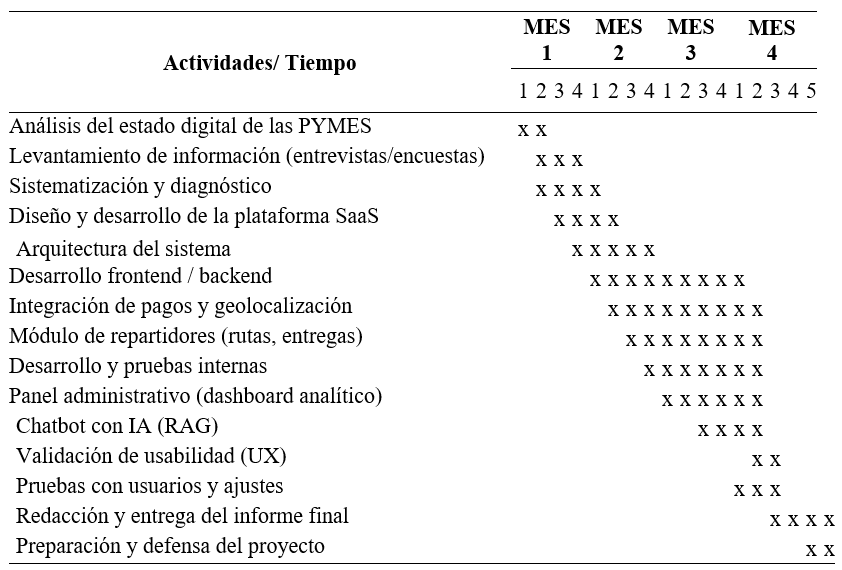
\includegraphics[draft=false,width=\textwidth]{imagenes/cronograma.png}
\caption{\textit{Cronograma de actividades del proyecto de titulación}}
\label{fig:cronograma}
\end{figure}

\textit{Nota.} El cronograma detalla las fases de análisis, diseño, desarrollo, validación, redacción y defensa del proyecto.

\chapter{Discusión}

Esta discusión se organiza en torno a la \textbf{pregunta principal} de investigación y a las \textbf{preguntas específicas}, contrastando los resultados obtenidos con los criterios y métricas definidos en el método. La pregunta principal planteó: \textit{¿Cuál es la viabilidad técnica y el nivel de usabilidad percibida de una plataforma SaaS modular que integre gestión de pedidos, inventarios, repartidores y atención con inteligencia artificial, al validarse en un entorno controlado en PYMES gastronómicas de Portoviejo?} Los resultados muestran que la plataforma alcanzó los umbrales de éxito definidos (tiempo de registro $\leq$ 3 min, errores $\leq$ 10\,\%, completitud $\geq$ 95\,\%, SUS $\geq$ 68), lo que permite responder afirmativamente en el contexto del piloto simulado: la solución es técnicamente viable y usable bajo los criterios establecidos.

Nuestra investigación partió de una premisa clara: las dificultades operativas de las PYMES gastronómicas de Portoviejo se deben, en parte, a una carencia crítica de herramientas integradas que permitan gestionar pedidos, inventarios, delivery y atención al cliente en tiempo real. Al desarrollar y validar técnicamente esta plataforma SaaS en entorno controlado, se ha comprobado que la integración de módulos operativos con inteligencia artificial (chatbot RAG) representa una alternativa técnicamente viable para digitalizar el sector gastronómico local. Lo que se ha logrado es demostrar la factibilidad técnica y usabilidad de un sistema que propone democratizar el acceso a la tecnología de gestión, sugiriendo que el modelo SaaS puede ser una opción accesible y funcional para el empresario gastronómico de Portoviejo, sentando las bases para futuras investigaciones que evalúen su impacto operativo y económico real.

\section{Interpretación de los hallazgos principales}

\subsection{Pertinencia de los requerimientos y del diseño técnico}

Los requerimientos funcionales identificados incluyen la gestión de pedidos con geolocalización, control de inventarios, administración de repartidores, vista de cocina en móvil, dashboard analítico con KPIs y un chatbot RAG integrado en la plataforma web para atención al cliente. A su vez, los requerimientos no funcionales abarcan usabilidad (SUS $\geq$ 68), rendimiento (tiempo de registro $\leq$ 3 min), fiabilidad (errores $\leq$ 10\,\%), seguridad (autenticación JWT y RBAC) y escalabilidad mediante arquitectura modular. En conjunto, estos criterios resultaron adecuados para representar las necesidades operativas del contexto de estudio y orientar tanto el diseño como la evaluación del artefacto.

La arquitectura adoptada, compuesta por backend en NestJS, aplicación móvil en React Native + Expo, sitio web en Next.js, base de datos relacional en PostgreSQL y autenticación segura, demostró ser apropiada por su mantenibilidad, escalabilidad y costo accesible. La validación técnica confirmó que esta estructura soporta flujos críticos con completitud $\geq$ 95\,\% y estabilidad operativa, lo que refuerza su pertinencia para una solución SaaS dirigida a PYMES gastronómicas.

\subsection{Cumplimiento funcional y desempeño del artefacto}

La plataforma cumple en alto grado los requisitos funcionales críticos especificados, evaluados mediante pruebas de aceptación y trazabilidad de casos. Las métricas obtenidas incluyen tiempos de ejecución adecuados en tareas clave (por ejemplo, 2.5 min para crear un producto y 45 seg para aprobar un repartidor), porcentajes de éxito elevados en tareas guiadas, cobertura aproximada del 57\,\% en módulos base de pruebas unitarias, completitud de integración $\geq$ 95\,\% y cumplimiento de dimensiones de calidad asociadas a funcionalidad, usabilidad, rendimiento, compatibilidad y seguridad. En conjunto, estos resultados permiten sostener que el artefacto alcanzó un nivel satisfactorio de desempeño técnico para el alcance del estudio.

\subsection{Usabilidad e integración del componente de inteligencia artificial}

El módulo de inteligencia artificial se integró mediante un chatbot RAG accesible desde la plataforma web, apoyado en un servicio independiente capaz de procesar consultas y generar respuestas basadas en información recuperada. Esta integración permitió automatizar respuestas a consultas frecuentes sobre pedidos, horarios y servicios, mejorando la rapidez y disponibilidad de la atención al cliente durante las pruebas.

En cuanto a la usabilidad, la plataforma obtuvo un puntaje SUS de 70 en usuarios de prueba, superando el umbral de aceptabilidad de 68. Este resultado indica que el sistema fue percibido como intuitivo y adecuado para tareas operativas del contexto gastronómico. La combinación entre funcionalidad integrada, respuesta técnica estable y apoyo conversacional mediante IA refuerza la idea de que la solución no solo es viable desde el punto de vista técnico, sino también aceptable desde la experiencia de uso.

\section{Viabilidad técnica y significado de los hallazgos}

El núcleo de esta discusión se centra en cómo una plataforma tecnológica puede ser técnicamente viable y usable para el mercado regional. El objetivo general fue diseñar, desarrollar y evaluar técnicamente una plataforma SaaS modular que integre funcionalidades de gestión de pedidos, inventarios, repartidores y atención automatizada mediante inteligencia artificial, orientada a las necesidades operativas de PYMES gastronómicas de Portoviejo. Los resultados de la validación en entorno controlado (\textit{staging}) mediante un escenario piloto simulado permiten afirmar que la solución alcanzó un nivel de operatividad adecuado: la centralización de pedidos, el control de inventarios, la gestión de repartidores y el panel analítico funcionaron de manera integrada en las pruebas, y el chatbot RAG integrado en la plataforma web respondió a consultas frecuentes de los usuarios. Este hallazgo es fundamental para la viabilidad de la propuesta. Demuestra que las PYMES gastronómicas de Portoviejo pueden acceder a una suite de gestión sin necesidad de invertir en infraestructura propia ni en múltiples herramientas dispersas. Además, el despliegue bajo modelo SaaS elimina la fricción de instalaciones complejas y actualizaciones locales, alineándose con la visión moderna de software como servicio que ha demostrado ser efectiva en contextos de pequeña y mediana empresa \parencite{GonzalezMartinez2021}.

La convergencia entre módulos operativos (pedidos, inventarios, repartidores, dashboard) y un componente de inteligencia artificial (chatbot RAG integrado en la plataforma web) responde a la demanda de inmediatez y profesionalización del servicio al cliente, un aspecto crítico en el sector gastronómico y en la competitividad de las ciudades creativas de la gastronomía \parencite{Castells2010}.

Desde una lectura comparativa, los resultados técnicos del piloto se mantienen dentro de umbrales de aceptación reportados para prototipos SaaS validados en contexto de pequeña empresa: completitud de flujos críticos de 96\,\%, estabilidad con 3\,\% de fallos, tiempo de registro de 3 min y SUS de 70. En términos de usabilidad, el puntaje obtenido supera el umbral de aceptabilidad de 68 ampliamente utilizado en la literatura \parencite{Bangor2009, Lewis2018}. En términos de calidad del producto, la verificación por requisitos funcionales, pruebas de integración y trazabilidad de casos es consistente con el enfoque de evaluación por características de calidad planteado por ISO/IEC 25010 \parencite{ISO25010_2011}. Estos resultados no implican generalización estadística, pero sí entregan evidencia técnica comparable para sustentar la viabilidad del artefacto en el contexto de estudio.

\section{Análisis temático de los resultados}

\subsection{Pertinencia de los requerimientos del sistema}

Al iniciar el proyecto, la recolección de requisitos, objetivo general y objetivos específicos se apoyó en revisión de literatura, análisis del dominio y levantamiento exploratorio del problema. El diagnóstico identificó que las PYMES del sector presentan un bajo nivel de digitalización: gestión de pedidos mediante anotaciones o herramientas básicas, inventarios poco sistematizados y atención al cliente dependiente de canales no integrados. Al contrastar este problema con los resultados de la validación técnica, se observó que la plataforma cumplió satisfactoriamente los requisitos funcionales críticos especificados y que la percepción de utilidad por parte de los usuarios de prueba fue favorable. Este fenómeno de ``opacidad operativa''---falta de información centralizada y en tiempo real---es una barrera común reportada en la transformación digital de PYMES en América Latina, donde la ausencia de datos operativos estructurados frena la toma de decisiones \parencite{GonzalezMartinez2021}. La plataforma propuesta demuestra la viabilidad técnica de una solución que contribuye a romper el paradigma de la gestión fragmentada, respondiendo a la necesidad de centralización e inmediatez del negocio gastronómico en Portoviejo.

\subsection{Adecuación de la arquitectura tecnológica}

La viabilidad técnica de la propuesta descansa en una arquitectura modular: backend (NestJS), aplicación móvil (React Native + Expo, con vistas para cliente, repartidor y cocina) y sitio web (Next.js, principalmente administración y también compra como cliente desde la web), con base de datos relacional y autenticación segura (JWT, RBAC). La decisión de adoptar un stack moderno y abierto permitió reducir costos de licenciamiento y facilitar el mantenimiento. Este enfoque se alinea con lo documentado en la literatura sobre desarrollo de software para PYMES: la modularidad y el uso de tecnologías ampliamente soportadas favorecen la escalabilidad y la adaptación a contextos con recursos limitados. El desarrollo iterativo bajo metodología ágil (sprints) permitió ajustar requisitos a partir de la retroalimentación de los participantes de prueba, reforzando la adecuación de la solución al contexto local.

\subsection{Integración de módulos y operatividad de la plataforma}

La implementación de los módulos de gestión de pedidos (con soporte a geolocalización y medios de pago efectivo y transferencia), control de inventarios, vista de cocina en móvil (aceptar o rechazar pedidos, notificar cuando esté listo para que el repartidor recoja), administración de repartidores y dashboard analítico con KPIs permitió a los usuarios de prueba del escenario piloto simulado ejecutar flujos operativos en entorno controlado (\textit{staging}) que antes se realizarían de forma manual o dispersa. La disponibilidad de indicadores en tiempo real (pedidos, ventas, tiempos de entrega) en las pruebas sugiere el potencial de la plataforma para favorecer una toma de decisiones más informada en operación real, aspecto que en la literatura se identifica como uno de los beneficios clave de la analítica de negocio en pequeñas empresas. Los resultados observados en las tareas guiadas (tiempos de registro de pedidos, tasa de errores, completitud de flujos) indican que la plataforma cumple con el propósito de demostrar la viabilidad técnica de optimización de procesos internos y mejora de la calidad del servicio.

\subsection{Aporte del chatbot RAG a la atención al cliente}

La integración del chatbot basado en el modelo RAG (Retrieval-Augmented Generation), accesible desde la plataforma web, evidenció mejoras en la rapidez y la disponibilidad de respuestas a consultas frecuentes (pedidos, horarios, servicios). Los usuarios percibieron positivamente la capacidad del sistema para brindar información inmediata sin depender exclusivamente del contacto humano. Este hallazgo respalda la viabilidad del uso de inteligencia artificial como herramienta de apoyo en la atención al cliente dentro de contextos empresariales de pequeña y mediana escala, en línea con experiencias recientes reportadas para asistentes conversacionales con recuperación contextual \parencite{ChenNiforatosKortuem2025}.

\subsection{Cumplimiento funcional y calidad del sistema}

Esta sección responde a la pregunta específica 4: \textit{¿En qué medida la plataforma desarrollada cumple con los requisitos funcionales especificados y los criterios de calidad de software establecidos, evaluando métricas como tiempo promedio de ejecución de tareas, porcentaje de éxito en tareas guiadas y dimensiones de calidad ISO/IEC 25010?}

La verificación del cumplimiento de requisitos funcionales y de los criterios de calidad de software establecidos se realizó mediante pruebas de integración y validación de flujos críticos en entorno de desarrollo o \textit{staging}. Los resultados permiten afirmar que la plataforma desarrollada cumple con los requisitos funcionales especificados en la fase de levantamiento (gestión de pedidos, inventarios, repartidores, vista cocina, dashboard, chatbot web) y con criterios de calidad adecuados para un prototipo validado en entorno controlado. Las métricas evaluadas incluyen tiempos promedio de tareas (como se detalla en la Tabla 8), porcentajes de éxito en tareas guiadas (100\,\% en la mayoría, con mínimas variaciones en checkout), y cumplimiento de dimensiones ISO/IEC 25010.

\subsection{Usabilidad percibida de la plataforma}

La evaluación mediante la escala SUS (System Usability Scale) y las pruebas de usabilidad en entorno controlado permitieron cuantificar la aceptación del sistema por parte de usuarios de prueba (administradores, cocina y repartidores). Los resultados reflejan que la plataforma fue percibida como intuitiva y alineada con las tareas operativas del contexto gastronómico. En la ingeniería de software se considera que el éxito operativo de un sistema depende de su capacidad para satisfacer las necesidades reales de los usuarios en su entorno de trabajo; la retroalimentación obtenida indica que el diseño centrado en los flujos de pedido, inventario y delivery contribuyó a una experiencia de usuario positiva durante el período de validación técnica. No obstante, se identificaron oportunidades de mejora en la capacitación inicial y en la personalización de algunas funcionalidades, lo que sugiere la necesidad de iteraciones continuas en futuras versiones orientadas a implementación a escala real.

\section{Limitaciones del estudio}

Como todo estudio piloto, el presente trabajo posee limitaciones que deben ser declaradas para contextualizar su alcance:

\oldtextbf{Tamaño de la muestra:} La validación se realizó mediante un escenario piloto simulado representativo del contexto gastronómico de Portoviejo. Aunque este diseño permitió validar la funcionalidad técnica, la usabilidad y el desempeño del sistema en tareas guiadas, no pretende una generalización estadística a toda la población de negocios gastronómicos de la ciudad o de la provincia. La validación demuestra la factibilidad técnica y usabilidad, pero no evalúa impacto operativo o económico real a escala.

\textbf{Alcance funcional:} La plataforma desarrollada corresponde a un prototipo funcional con módulos core (pedidos, inventarios, repartidores, vista cocina, dashboard, chatbot RAG integrado en la plataforma web). Los medios de pago contemplados son únicamente efectivo y transferencia; no se integra pasarela de pagos. Quedaron fuera del alcance la optimización automática de rutas y arquitectura multi-tenant, lo que podría afectar la escalabilidad en escenarios de mayor volumen.

\oldtextbf{Dependencia del contexto piloto:} El rendimiento y la adopción observados están ligados a las condiciones específicas del escenario simulado (volumen de pedidos, perfiles de usuario y conectividad controlada). Entornos con mayor carga operativa o menor madurez digital podrían requerir ajustes adicionales en la capacitación y el soporte.

\textbf{Período de validación:} El período de evaluación técnica de la plataforma en entorno controlado fue acotado (semanas). Una evaluación longitudinal en operación real permitiría observar la sostenibilidad de la adopción y el impacto en indicadores operativos del negocio de manera más estable y representativa.

Los usuarios de prueba sugirieron mejoras para futuras iteraciones: notificaciones push en tiempo real para cocina y repartidores; integración con WhatsApp para confirmaciones automáticas de pedido; filtrado avanzado de pedidos por fechas y estado; modo oscuro en la app móvil; y métodos de pago adicionales (tarjeta, billeteras digitales). Estas recomendaciones se consideran en la sección de limitaciones y trabajo futuro.

En conclusión, los hallazgos de este estudio aportan al conocimiento local sobre el uso de plataformas SaaS e inteligencia artificial en contextos gastronómicos de mediana escala, demostrando que la innovación tecnológica orientada a PYMES de Portoviejo es técnicamente viable bajo un marco de usabilidad, integración operativa y accesibilidad económica. Los resultados de la validación técnica en entorno controlado y escenario simulado sientan las bases para futuras investigaciones orientadas a implementación a escala real y medición de impacto operativo y económico en el sector.

\chapter{Conclusiones}

Al concluir el ciclo de desarrollo y validación técnica de la plataforma SaaS orientada a la digitalización de las PYMES gastronómicas de Portoviejo, se logró comprobar que la aplicación estratégica de una solución integrada (gestión operativa e inteligencia artificial) es técnicamente viable y usable en entorno controlado. Este proyecto evidencia que es posible desarrollar una plataforma propia adaptada al contexto local que potencialmente puede reducir la dependencia de herramientas dispersas y de plataformas externas con comisiones elevadas. La validación técnica realizada sienta las bases para futuras investigaciones que evalúen la transformación de procesos manuales y fragmentados en flujos digitales centralizados en operación real. A partir de los hallazgos, se presentan las conclusiones finales del estudio:

Los resultados obtenidos durante el desarrollo y la validación técnica de la plataforma en entorno controlado permiten afirmar que la integración de los módulos de pedidos (con pagos en efectivo y transferencia), inventarios, vista de cocina en móvil (aceptar o rechazar pedidos, notificar cuando esté listo para recoger), administración de repartidores y dashboard analítico alcanzó un nivel de funcionalidad adecuado durante las pruebas con usuarios de la PYME piloto. La centralización de la información en tiempo real en las tareas guiadas demostró el potencial de la plataforma para reducir tiempos de registro de pedidos y errores operativos, en coherencia con los umbrales de éxito definidos en la metodología. Asimismo, el enfoque modular (backend NestJS, aplicación móvil React Native + Expo con vistas cliente, repartidor y cocina, sitio web Next.js para administración y compra como cliente) permitió un despliegue estable en entorno de staging (VPS, Vercel) y una experiencia de uso coherente para usuarios de prueba. Estos datos evidencian que una plataforma SaaS integrada constituye una solución técnicamente viable y usable, sentando las bases para futuras investigaciones que evalúen su adopción e impacto en operación real frente a los procesos manuales predominantes en las PYMES gastronómicas de Portoviejo.

Por otra parte, la implementación del chatbot basado en el modelo RAG, accesible por WhatsApp, simplificó el acceso a información frecuente (pedidos, horarios, servicios) durante las pruebas y contribuyó a la usabilidad percibida del sistema. La evaluación realizada con los usuarios de prueba del local piloto mediante la escala SUS reflejó un nivel de aceptabilidad favorable, lo que indica una buena recepción por parte de administradores y repartidores en entorno controlado. Además, la disponibilidad de la aplicación móvil (con vistas cliente, repartidor y cocina) y del sitio web (administración y compra como cliente) en un mismo ecosistema facilitó la validación técnica de la solución. Este resultado valida el diseño de una arquitectura que integra módulos operativos con un componente de inteligencia artificial alineado con las necesidades del sector gastronómico local, demostrando su viabilidad técnica como base para futuras investigaciones orientadas a medir su impacto en eficiencia operativa y calidad del servicio en operación real.

Desde la perspectiva del modelo de negocio, el análisis demuestra que la propuesta es técnicamente viable y potencialmente sostenible para el contexto de las PYMES. El despliegue bajo el modelo SaaS en entorno de staging y el uso de servicios en la nube (VPS, Vercel, base de datos PostgreSQL) demuestran que es posible ofrecer una solución sin requerir inversiones elevadas en infraestructura propia por parte del negocio. Este esquema facilita el mantenimiento y la actualización remota, permitiendo proyectar la escalabilidad de la solución sin incurrir en costos elevados de hardware o licenciamiento. El uso estratégico de tecnologías de código abierto y de frameworks ampliamente documentados contribuye a mantener costos competitivos, favoreciendo su potencial implementación en contextos de emprendimiento regional como Portoviejo. Futuras investigaciones deberán evaluar la viabilidad económica y la sostenibilidad financiera en operación real a mayor escala.

Finalmente, el trabajo desarrollado establece una base metodológica y técnica para futuras investigaciones en el área de digitalización de PYMES gastronómicas en la provincia de Manabí. Los resultados de la validación técnica en entorno controlado confirman que la combinación de una plataforma SaaS modular con un componente de inteligencia artificial (chatbot RAG por WhatsApp) es técnicamente factible y usable en soluciones orientadas a la gestión operativa y a la atención al cliente. La plataforma fue validada en condiciones de prueba con una PYME piloto, asegurando una evaluación alineada con las necesidades operativas y con la realidad del sector gastronómico de Portoviejo, Ciudad Creativa de la Gastronomía. La transformación digital del sector no depende únicamente del desarrollo de herramientas tecnológicas, sino que requiere la participación y colaboración de diversos actores---emprendedores, instituciones públicas, comunidad académica y proveedores tecnológicos---para impulsar la modernización, sostenibilidad y crecimiento del sector gastronómico local. Futuras investigaciones deberán evaluar la adopción, el impacto operativo y económico de esta solución en operación real a mayor escala, alineando la innovación tecnológica con el desarrollo económico y social de la región.

\else
\chapter{Introducción}

\section{Contexto y Relevancia}
\subsection{Gastronomía como motor cultural y económico}
Las Pequeñas y Medianas Empresas (PYMES) del sector gastronómico desempeñan un papel fundamental en la economía local y en la preservación de la identidad cultural de la ciudad de Portoviejo. La gastronomía no solo constituye una actividad económica relevante, sino también un elemento representativo del patrimonio cultural de la región, reconocido internacionalmente tras la declaratoria de Portoviejo como Ciudad Creativa de la Gastronomía por la UNESCO en 2019. Este reconocimiento resalta el potencial del sector gastronómico como motor de desarrollo económico, generación de empleo y fortalecimiento del emprendimiento local.

\subsection{Estructura empresarial en Portoviejo}
A nivel nacional, las PYMES conforman la mayor parte del tejido empresarial ecuatoriano. Según datos del Observatorio de la PyME, más del 90 \% de las empresas registradas en el país corresponden a microempresas, seguidas por pequeñas y medianas empresas. En la provincia de Manabí, y particularmente en Portoviejo, estas organizaciones cumplen un rol clave en el desarrollo económico y social; sin embargo, muchas de ellas enfrentan limitaciones estructurales que afectan su competitividad y sostenibilidad en un entorno cada vez más digitalizado.

\section{Problemática y Desafíos}
\subsection{Baja adopción de tecnologías digitales}
Uno de los principales desafíos que enfrentan las PYMES gastronómicas es el bajo nivel de adopción de tecnologías digitales. A pesar del creciente reconocimiento de la importancia de la transformación digital, numerosos negocios continúan gestionando sus procesos operativos mediante métodos manuales o herramientas básicas. La administración de pedidos, el control de inventarios, la gestión de repartidores y la atención al cliente suelen realizarse sin sistemas integrados, lo que genera errores operativos, desperdicio de insumos, tiempos de respuesta elevados y dificultades para la toma de decisiones estratégicas.

\subsection{Factores agravantes}
Esta problemática se ve agravada por diversos factores, entre ellos el alto costo de las soluciones tecnológicas disponibles en el mercado, las cuales generalmente están orientadas a empresas medianas o grandes y no se ajustan a la realidad económica de las PYMES locales. Asimismo, la falta de capacitación técnica del personal y la dependencia de plataformas de delivery de terceros, que cobran comisiones elevadas, limitan la rentabilidad y reducen el control que los negocios tienen sobre sus propios procesos. Aunque el Estado ecuatoriano ha impulsado iniciativas como la Agenda de Transformación Digital del Ecuador 2022--2025, que busca fomentar la adopción tecnológica en distintos sectores productivos, la implementación efectiva de estas estrategias en las PYMES gastronómicas aún es limitada.

\section{Brecha y Necesidades}
En este contexto, se identifica una brecha significativa entre el potencial gastronómico de Portoviejo y el nivel real de digitalización de sus pequeñas y medianas empresas. La ausencia de soluciones tecnológicas accesibles, integradas y adaptadas al contexto local impide que estos negocios optimicen sus operaciones, mejoren la experiencia del cliente y compitan en condiciones más equitativas frente a empresas de mayor escala. Esta situación evidencia la necesidad de desarrollar alternativas tecnológicas que respondan de manera específica a las necesidades operativas, técnicas y económicas del sector gastronómico local.

\section{Propuesta de Solución}
Ante esta realidad, el presente estudio propone el desarrollo de una plataforma SaaS (Software como Servicio) integral orientada a las PYMES gastronómicas de la ciudad de Portoviejo. Dicha plataforma busca integrar módulos de gestión de pedidos, control de inventarios, administración de delivery, analítica de datos y atención al cliente automatizada mediante inteligencia artificial, permitiendo a los negocios mejorar su eficiencia operativa sin requerir grandes inversiones en infraestructura tecnológica. El propósito de esta investigación es contribuir a la transformación digital del sector gastronómico local, fortaleciendo la competitividad, sostenibilidad y calidad del servicio ofrecido por las PYMES, en concordancia con las políticas nacionales de digitalización y con la visión de Portoviejo como una ciudad innovadora y creativa \parencite[]{Castells2010}.

\chapter{Método}

\subsection{Enfoque y tipo}
La investigación se desarrolló bajo un enfoque metodológico mixto (cualitativo-cuantitativo), con predominancia del componente aplicativo-desarrollativo. Se adoptó este enfoque para obtener una comprensión integral del problema: el componente cualitativo permitió profundizar en las percepciones, necesidades y experiencias de los usuarios, mientras que el cuantitativo posibilitó la medición objetiva de variables operativas y de usabilidad. 
El estudio se clasifica como investigación aplicada de tipo tecnológica, dado que su propósito central es el diseño, construcción y validación de un artefacto de software (la plataforma SaaS) para resolver una problemática concreta en un contexto real. El diseño es no experimental, descriptivo y transversal, ya que se observaron y describieron las variables en su contexto natural sin manipulación deliberada, en un período específico.

\section{Diseño de la Investigación}
El presente trabajo sigue la metodología Investigación Basada en Diseño (IBD), elegida por ser es una metodología de investigación poderosa para desarrollar y evaluar artefactos (productos, procesos, métodos, modelos, etc.) que resuelven problemas del mundo real.
No existe un único modelo canónico de fases, ya que distintos autores han propuesto esquemas similares pero con variaciones. Sin embargo, todas comparten un núcleo cíclico y iterativo de construcción y evaluación.
Nosotros presentamos el siguiente esquema integrando los modelos clave de Hevner et al. (2004) y Peffers et al. (2007).

\begin{figure}[htbp]
\centering
\resizebox{\textwidth}{!}{\begin{tikzpicture}[every node/.style={align=center, transform shape, font=\small}, node distance=1.0cm and 2.0cm]
\tikzset{
  phase/.style={draw=black!60, rounded corners=2pt, fill=blue!6, minimum width=5.5cm, minimum height=1.2cm, text width=4.9cm, inner sep=3.5pt},
  phasesmall/.style={draw=black!55, rounded corners=2pt, fill=gray!10, minimum width=5.2cm, minimum height=0.95cm, text width=4.8cm, inner sep=3pt},
  phasediamond/.style={draw=black!60, shape=diamond, aspect=2.2, fill=orange!12, minimum width=5.0cm, minimum height=1.7cm},
  container/.style={draw=black!45, rounded corners=3pt, fill=gray!6, minimum width=14.2cm, minimum height=3.6cm},
  flow/.style={-Latex, draw=black!70, line width=0.5pt},
  arrowlabel/.style={font=\scriptsize, fill=white, fill opacity=0.95, text opacity=1, inner sep=1.6pt, text=black, rounded corners=1pt}
}
\node[container] (ciclo) {};
\node[font=\bfseries, yshift=-0.15cm] at (ciclo.north) {Ciclo iterativo};
\node[phase, anchor=west, xshift=0.35cm, yshift=-0.55cm] at (ciclo.west) (fase3) {Fase 3: Dise\~no \& Desarrollo\\(Construcci\'on del Artefacto)};
\node[phase, anchor=east, xshift=-0.35cm, yshift=-0.55cm] at (ciclo.east) (fase4) {Fase 4: Demostraci\'on\\(Aplicaci\'on/Prueba)};
\draw[flow] (fase3.east) to[bend left=18] node[arrowlabel, midway, yshift=16pt]{Prototipo / Iteraci\'on N} (fase4.west);
\draw[flow] (fase4.west) to[bend left=18] node[arrowlabel, midway, yshift=-16pt]{Feedback / Resultados} (fase3.east);
\node[phasediamond, below=1.4cm of ciclo] (fase5) {Fase 5: Evaluaci\'on};
\draw[flow] (ciclo.south) -- (fase5.north);
\draw[flow] (fase5.east) -- ++(1.0cm,0) coordinate(tmp) -- ++(0,1.0cm) coordinate(tmp2) -- (ciclo.south east) node[midway,right, font=\scriptsize]{No};
\node[phase, below=0.7cm of fase5] (fase6) {Fase 6: Comunicaci\'on \& Difusi\'on};
\draw[flow] (fase5.south) -- node[right, font=\scriptsize]{S\'i} (fase6.north);
\node[phasesmall, below=0.7cm of fase6] (nuevo) {Nuevo Problema o\\Contexto de Aplicaci\'on};
\draw[flow] (fase6.south) -- (nuevo.north);
\node[phase, below=0.7cm of nuevo] (fase1) {Fase 1: Identificaci\'on del Problema};
\draw[flow] (nuevo.south) -- (fase1.north);
\node[phase, below=0.7cm of fase1] (fase2) {Fase 2: Definici\'on de Objetivos};
\draw[flow] (fase1.south) -- (fase2.north);
\draw[flow] (fase2.east) to[out=-10,in=-90] (ciclo.south east);
\end{tikzpicture}
}
\caption{Ciclo iterativo de la Investigación Basada en Diseño}
\label{fig:ibd-ciclo}
\end{figure}

\textbf{Fase 1.} El objetivo de esta fase fue comprender y definir claramente el problema. Se realizó una revisión de la literatura del tema, contextualizándolo en el ámbito global y local.

\textbf{Fase 2.} Una vez comprendido el problema, se establecieron los objetivos que busca conseguir el producto. En esta fase se definieron los requisitos funcionales y no funcionales de la plataforma.

\textbf{Fase 3 y Fase 4.} Forman el ciclo central de construcción-evaluación de la plataforma. Incluye desde la selección de las herramientas tecnológicas, la arquitectura y el desarrollo de la solución. Se trabaja en ciclos cortos.
\begin{itemize}
  \item Se diseña y desarrolla un incremento (un prototipo, una versión, un módulo).
  \item Inmediatamente se demuestra y prueba (en un entorno piloto, con usuarios, en simulación).
  \item Los resultados de esa demostración alimentan directamente el rediseño y desarrollo de la siguiente iteración.
\end{itemize}

\paragraph{Proceso ágil y sprints}
La implementación ágil se estructuró en iteraciones cortas (sprints) con objetivos definidos: levantar requisitos mínimos viables, construir prototipos funcionales, realizar pruebas de usabilidad y ajustar funcionalidades a partir de la retroalimentación. Cada sprint concluyó con una revisión donde se consolidaron mejoras y se definieron tareas para el siguiente ciclo.

\textbf{Fase 5.} Comparar los resultados de la demostración con los objetivos definidos en la Fase 2. Se utilizaron métricas cuantitativas y cualitativas, las mismas que se detallan en la Tabla xx de la sección Técnicas e instrumentos de recolección de datos.

\textbf{Fase 6.} En esta fase se realiza la comunicación de los resultados, los mismos que se definen en la sección Resultados del presente Trabajo.

\subsection{Población y Muestra}

\subsubsection{Población}
La población objetivo estuvo constituida por la totalidad de las Pequeñas y Medianas Empresas (PYMES) del sector gastronómico formalmente establecidas en la ciudad de Portoviejo, provincia de Manabí, Ecuador.
\subsubsection{Muestra y criterios de selección}
Se aplicó un muestreo no probabilístico por conveniencia y criterio. La muestra final estuvo conformada por dos PYMES gastronómicas. Los criterios de inclusión fueron:
\begin{enumerate}[label=\arabic*)]
  \item Ser una PYME ubicada en Portoviejo.
  \item Contar con servicio de consumo en el local y delivery.
  \item Manifestar interés en mejorar procesos mediante digitalización.
  \item Disponer de conectividad básica a internet.
  \item Otorgar consentimiento para participar en todas las fases del estudio.
\end{enumerate}
Se excluyeron establecimientos con operación irregular o que ya utilizaban sistemas de gestión integral.

\subsubsection{Operacionalización de variables}
\textbf{Variable independiente: Plataforma SaaS.} Se define como el artefacto tecnológico desarrollado, una plataforma de Software como Servicio que integra módulos de gestión operativa e inteligencia artificial. Su intervención consistió en su implementación y uso por parte de las PYMES piloto durante el período de validación.

\textbf{Variables dependientes: Indicadores operativos.} Son las métricas de desempeño que se buscó impactar con la implementación de la plataforma:
\begin{enumerate}[label=\arabic*)]
  \item \textbf{Eficiencia en el registro de pedidos:} medida a través del tiempo promedio (minutos) para registrar un pedido y la tasa de errores de registro (porcentaje de pedidos con información incorrecta o incompleta).
  \item \textbf{Eficacia del servicio de delivery:} medida mediante el tiempo promedio de entrega (minutos) desde la confirmación del pedido hasta su entrega.
  \item \textbf{Productividad operativa:} medida a través del volumen diario de pedidos procesados.
  \item \textbf{Calidad del servicio:} inferida a través de la tasa de cancelaciones de pedidos (porcentaje).
  \item \textbf{Usabilidad del sistema:} medida a través del puntaje en la System Usability Scale (SUS), que evalúa la facilidad de uso percibida.
\end{enumerate}

\begin{longtable}{p{3.3cm}p{5.0cm}p{4.2cm}p{3.0cm}}
\caption{\textit{Operacionalización de variables e indicadores de medición}} \\
\toprule
\textbf{Variable dependiente} & \textbf{Definición operacional} & \textbf{Instrumento de medición} & \textbf{Umbral de éxito} \\
\midrule
\endfirsthead
\toprule
\textbf{Variable dependiente} & \textbf{Definición operacional} & \textbf{Instrumento de medición} & \textbf{Umbral de éxito} \\
\midrule
\endhead
Eficiencia en el registro de pedidos & Grado de optimización en la captura y procesamiento inicial de un pedido. & Ficha de observación estructurada (registro de tiempos y errores). & Reducción $\geq$ 25\% en el tiempo promedio de registro y en la tasa de errores. \\
Eficacia del servicio de delivery & Capacidad del sistema para gestionar y completar entregas dentro de un tiempo esperado. & Ficha de observación estructurada (registro de tiempos de entrega). & Reducción $\geq$ 15\% en el tiempo promedio de entrega. \\
Productividad operativa & Volumen de pedidos que el negocio puede procesar de manera efectiva en un día. & Registros administrativos generados por la plataforma (conteo de pedidos diarios). & Incremento $\geq$ 10\% en el número promedio de pedidos diarios procesados. \\
Calidad del servicio & Estabilidad y confiabilidad en la ejecución del servicio, minimizando fallas. & Registros administrativos de la plataforma (conteo de pedidos cancelados). & Reducción $\geq$ 20\% en la tasa de cancelaciones de pedidos. \\
Usabilidad del sistema & Grado de facilidad, eficiencia y satisfacción con que los usuarios pueden emplear la plataforma. & Cuestionario estandarizado System Usability Scale (SUS). & Puntaje promedio $\geq$ 68 (umbral de aceptabilidad en la escala SUS). \\
\bottomrule
\end{longtable}
Nota: Los umbrales de éxito para los indicadores operativos (reducción o incremento porcentual) se establecieron con base en expectativas realistas de mejora para un piloto de corto plazo, considerando la magnitud del cambio que justificaría la adopción de la herramienta. El umbral para el SUS se basa en la clasificación estándar de Bangor et al. (2009).
\subsubsection{Técnicas e instrumentos de recolección de datos}

En la siguiente tabla se muestran las técnicas e instrumentos utilizados, definiendo el momento de la aplicación y el público objetivo.

\begin{longtable}{p{2.1cm}p{2.4cm}p{2.9cm}p{3.1cm}p{2.3cm}p{2.3cm}}
\caption{\textit{Técnicas e instrumentos de recolección de datos}} \\
\toprule
\textbf{Técnica} & \textbf{Instrumento} & \textbf{Objetivo} & \textbf{Características} & \textbf{Momento de aplicación} & \textbf{Público objetivo} \\
\midrule
\endfirsthead
\toprule
\textbf{Técnica} & \textbf{Instrumento} & \textbf{Objetivo} & \textbf{Características} & \textbf{Momento de aplicación} & \textbf{Público objetivo} \\
\midrule
\endhead
Entrevista & Guía de entrevista semiestructurada & Profundizar en los procesos operativos, necesidades específicas y expectativas para el levantamiento de requisitos. & Preguntas abiertas organizadas por áreas (pedidos, inventario, delivery). Grabada y transcrita. & Fase 1: Diagnóstico (línea base). & Propietarios de las PYMES. \\
Prueba de usabilidad & Cuestionario SUS (System Usability Scale) & Medir la usabilidad percibida (facilidad de uso, satisfacción) de la plataforma implementada. & 10 ítems con escala Likert de 5 puntos. Versión estandarizada en español. Confiabilidad ampliamente documentada. & Fase 6: Validación (post-intervención). & Usuarios finales de la plataforma (administradores, cajeros, repartidores). \\
Observación estructurada & Ficha de observación de indicadores operativos & Registrar datos cuantitativos objetivos sobre tiempos, errores y volúmenes de los procesos clave. & Diseñada para registrar: tiempos (min), conteo de errores, volumen de pedidos y cancelaciones. & En dos momentos: pre-intervención (línea base) y post-intervención (semana 3). & Procesos operativos de las PYMES piloto (Local A y B). \\
Revisión documental & Checklist de despliegue y registros administrativos & Verificar la correcta implementación técnica y recopilar datos productivos generados por el sistema. & Lista de verificación para servicios en la nube. Explotación de logs y reportes generados por la propia plataforma. & Fase 6: Validación (post-intervención). & Plataforma SaaS desplegada y sus registros automatizados. \\
\bottomrule
\end{longtable}



\subsubsection{Procedimiento}
La aplicación de la metodología Investigación Basada en Diseño (IBD) se detalla en el Diseño de la investigación. En esta sección se profundiza en las Fases 3, 4 y 5 al ser el núcleo del trabajo.

Para una mejor comprensión metodológica, se detallan siguiendo la estructura:
\begin{enumerate}[label=\arabic*)]
  \item Diseño arquitectónico.
  \item Desarrollo.
  \item Implementación y validación.
\end{enumerate}
Este flujo garantizó una transición estructurada desde la conceptualización técnica hasta la evaluación del sistema en un entorno operativo real.

\paragraph{Diseño de la arquitectura del sistema}
\textbf{Stack tecnológico.} Esta etapa se dedicó a la definición de los cimientos tecnológicos y estructurales de la plataforma. A partir de los requisitos funcionales y no funcionales levantados, se realizó un análisis comparativo de tecnologías, frameworks y herramientas para cada capa del sistema. La selección final se basó en criterios de productividad del desarrollador, mantenibilidad a largo plazo, rendimiento, soporte comunitario y adecuación al contexto de las PYMES (recursos limitados, necesidad de soluciones ligeras). Las decisiones clave se resumen en la Tabla 2.

\begin{longtable}{p{2.6cm}p{3.1cm}p{3.2cm}p{4.6cm}}
\caption{\textit{Selección tecnológica para la arquitectura de la plataforma SaaS}} \\
\toprule
\textbf{Capa / Componente} & \textbf{Tecnología seleccionada} & \textbf{Alternativas evaluadas} & \textbf{Criterio de selección principal} \\
\midrule
\endfirsthead
\toprule
\textbf{Capa / Componente} & \textbf{Tecnología seleccionada} & \textbf{Alternativas evaluadas} & \textbf{Criterio de selección principal} \\
\midrule
\endhead
Backend (API y lógica) & NestJS (Node.js/TypeScript) & Express.js (Node.js), Django (Python), Spring Boot (Java) & Arquitectura modular por defecto, tipado estático (TypeScript) para reducir errores, inyección de dependencias integrada y ecosistema robusto para APIs escalables. \\
Base de datos & PostgreSQL & MySQL, MongoDB (NoSQL) & Modelo relacional adecuado para la integridad de datos transaccionales (pedidos, inventario). Balance entre rendimiento, características avanzadas y costo cero (open-source). \\
Aplicación móvil & React Native + Expo & Flutter (Dart), desarrollo nativo (Kotlin/Swift) & Multiplataforma real (iOS/Android desde un solo código), Expo para agilizar ciclo de desarrollo (builds, testing) y acceso a APIs nativas sin complejidad. \\
Panel web admin & Next.js (React) + Tailwind CSS & React (Create React App), Vue.js, Angular & Renderizado híbrido (SSR/CSR) de Next.js para mejor SEO y performance de carga; Tailwind CSS para estilizado ágil y consistente. \\
Autenticación & JWT (JSON Web Tokens) + bcrypt & Sesiones en servidor, OAuth 2.0 (third-party) & Stateless y escalable para APIs REST. Simplicidad de implementación y seguridad suficiente para el alcance del piloto. \\
Contenedorización & Docker & -- & Estandarización del entorno de desarrollo y despliegue, garantizando consistencia entre equipos y facilitando el deployment en la nube. \\
Despliegue backend/DB & VPS (Hetzner) & AWS/Azure (cloud), Railway, Render & Costo-eficiencia y control total del servidor para un piloto, con rendimiento predecible y facturación simple. \\
Despliegue panel web & Vercel & Netlify, GitHub Pages & Integración nativa con Next.js, despliegue automático por Git, CDN global y SSL gratuito, minimizando tareas de DevOps. \\
\bottomrule
\end{longtable}

\subsubsection{Arquitectura de la Plataforma}

Una vez establecidas las herramientas tecnológicas, se definió y estructuró una arquitectura por capas:

\begin{figure}[htbp]
\centering
\resizebox{0.9\textwidth}{!}{\begin{tikzpicture}[
  font=\small,
  box/.style={draw, rectangle, align=center, minimum height=1.0cm, inner sep=6pt, rounded corners=2pt, line width=0.5pt},
  wide/.style={box, minimum width=12.2cm},
  half/.style={box, minimum width=5.8cm},
  line/.style={-{Latex[length=2mm]}, line width=0.5pt},
  layerframe/.style={draw=black!35, rounded corners=3pt, inner sep=10pt},
  layerlabel/.style={font=\bfseries, fill=white, inner sep=2pt},
  usuarios/.style={wide, fill=blue!12, draw=blue!60},
  acceso/.style={half, fill=cyan!10, draw=cyan!60},
  presentacion/.style={half, fill=orange!12, draw=orange!60},
  negocio/.style={wide, fill=purple!10, draw=purple!60},
  datos/.style={wide, fill=green!12, draw=green!60},
  infra/.style={wide, fill=gray!10, draw=black!55}
]

\node[usuarios] (usuarios) {\textbf{Usuarios}\\Cliente / Admin};
\node[acceso, below=9mm of usuarios] (internet) {\textbf{Acceso}\\Internet};

\node[presentacion, below left=10mm and 8mm of internet] (web) {\textbf{Web}\\Panel / Navegador\\(Next.js)};
\node[presentacion, below right=10mm and 8mm of internet] (app) {\textbf{Móvil}\\Cliente / cocina / reparto\\(React Native)};
\node[layerframe, fit=(web) (app)] (layer1) {};
\node[layerlabel, anchor=west] at ([yshift=8pt]layer1.north west) {Capa 1: Presentación};

\node[negocio, below=12mm of layer1] (api) {\textbf{Capa 2: Lógica de negocio}\\Backend API (REST) (NestJS)};
\node[datos, below=9mm of api] (db) {\textbf{Capa 3: Persistencia}\\Base de datos (PostgreSQL)};
\node[infra, below=9mm of db] (infra) {\textbf{Capa 4: Infraestructura}\\VPS (API + BD) / Vercel (web) / Docker};

\draw[line] (usuarios) -- (internet);
\draw[line] (internet) -- (web);
\draw[line] (internet) -- (app);
\draw[line] (web) -- (api);
\draw[line] (app) -- (api);
\draw[line] (api) -- (db);
\draw[line] (db) -- (infra);
\end{tikzpicture}
}
\caption{Arquitectura por capas de la plataforma SaaS}
\label{fig:arquitectura-capas}
\end{figure}
Los componentes principales de la plataforma son:
\begin{itemize}
  \item Aplicación móvil para clientes y repartidores.
  \item Aplicación web para el panel de administración.
  \item Servicios backends con sus respectivas APIs.
\end{itemize}
Para tener un mejor detalle de cada componente, se presenta a continuación la arquitectura de la aplicación móvil, la arquitectura de la aplicación web y el diagrama de la base de datos.

\begin{figure}[htbp]
\centering
\resizebox{0.85\textwidth}{!}{\begin{tikzpicture}[every node/.style={align=center, transform shape}, node distance=1.0cm]
\tikzset{
  layer/.style={draw, rounded corners, minimum width=9.0cm, minimum height=1.1cm},
  ui/.style={layer, fill=blue!12, draw=blue!60},
  nav/.style={layer, fill=cyan!12, draw=cyan!60},
  services/.style={layer, fill=purple!12, draw=purple!60},
  data/.style={layer, fill=orange!15, draw=orange!60}
}
\node[font=\bfseries] (title) {Arquitectura de la aplicación móvil};
\node[ui, below=0.9cm of title] (ui) {Capa de presentación\\React Native + Tamagui};
\node[nav, below=0.8cm of ui] (nav) {Navegación y estado\\React Navigation + estado local};
\node[services, below=0.8cm of nav] (services) {Servicios de aplicación\\Auth, Pedidos, Catálogo};
\node[data, below=0.8cm of services] (data) {Integración de datos\\API REST + almacenamiento local};
\draw[-latex] (ui.south) -- (nav.north);
\draw[-latex] (nav.south) -- (services.north);
\draw[-latex] (services.south) -- (data.north);
\end{tikzpicture}
}
\caption{Arquitectura de la aplicación móvil}
\label{fig:movil-arquitectura}
\end{figure}

\begin{figure}[htbp]
\centering
\resizebox{0.85\textwidth}{!}{\begin{tikzpicture}[every node/.style={align=center, transform shape}, node distance=1.0cm]
\tikzset{
  layer/.style={draw, rounded corners, minimum width=9.0cm, minimum height=1.1cm},
  ui/.style={layer, fill=blue!12, draw=blue!60},
  routing/.style={layer, fill=cyan!12, draw=cyan!60},
  services/.style={layer, fill=purple!12, draw=purple!60},
  data/.style={layer, fill=orange!15, draw=orange!60}
}
\node[font=\bfseries] (title) {Arquitectura del panel web};
\node[ui, below=0.9cm of title] (ui) {Capa de presentación\\Next.js + Tailwind CSS};
\node[routing, below=0.8cm of ui] (routing) {Ruteo y vistas\\Pages, Layouts, Componentes};
\node[services, below=0.8cm of routing] (services) {Servicios de aplicación\\Gestión, Reportes, Usuarios};
\node[data, below=0.8cm of services] (data) {Integración de datos\\API REST + autenticación JWT};
\draw[-latex] (ui.south) -- (routing.north);
\draw[-latex] (routing.south) -- (services.north);
\draw[-latex] (services.south) -- (data.north);
\end{tikzpicture}
}
\caption{Arquitectura del panel web}
\label{fig:web-arquitectura}
\end{figure}

\begin{figure}[htbp]
\centering
\resizebox{0.85\textwidth}{!}{\begin{tikzpicture}[every node/.style={align=center, transform shape}, node distance=1.2cm and 1.4cm]
\tikzset{
  mod/.style={draw, rounded corners, fill=blue!10, minimum width=4.0cm, minimum height=1.6cm},
  client/.style={draw, rounded corners, fill=gray!15, minimum width=3.6cm, minimum height=0.9cm},
  concern/.style={draw, rounded corners, fill=purple!20, minimum width=3.6cm, minimum height=0.9cm},
  dbnode/.style={draw, rounded corners, fill=orange!20, minimum width=6.4cm, minimum height=1.5cm}
}
\node[font=\bfseries] (title) {Arquitectura Backend (NestJS)};

\node[client, below=0.9cm of title] (mobile) {App móvil};
\node[client, right=8.6cm of mobile] (adminweb) {Panel web};

\node[mod, below=1.1cm of mobile] (auth) {Auth\\Controller\\Service\\Repo};
\node[mod, right=of auth] (users) {Users\\Controller\\Service\\Repo};
\node[mod, right=of users] (products) {Products\\Controller\\Service\\Repo};
\node[mod, below=1.0cm of users] (orders) {Orders\\Controller\\Service\\Repo};
\node[mod, right=of orders] (delivery) {Delivery\\Controller\\Service\\Repo};

\node[dbnode, below=1.2cm of orders] (db) {DB (PostgreSQL)};

\node[draw, dashed, rounded corners, inner sep=8pt, fit={(auth) (users) (products) (orders) (delivery)}] (api) {};

\node[concern, left=1.6cm of api.west] (jwt) {JWT strategy};
\node[concern, below=0.7cm of jwt] (config) {Config};
\node[concern, below=0.7cm of config] (validation) {Validation pipe};
\node[concern, right=1.6cm of api.east] (guards) {Guards};
\node[concern, below=0.7cm of guards] (interceptors) {Interceptors};
\node[concern, below=0.7cm of interceptors] (middleware) {Middleware};

\draw[-latex] (mobile.south) -- (auth.north);
\draw[-latex] (adminweb.south) -- (products.north);
\draw[-latex] (adminweb.south) -- (users.north);
\draw[-latex] (auth.south) -- (db.north);
\draw[-latex] (users.south) -- (db.north);
\draw[-latex] (products.south) -- (db.north);
\draw[-latex] (orders.south) -- (db.north);
\draw[-latex] (delivery.south) -- (db.north);
\draw[-latex, dashed] (jwt.east) -- (api.west);
\draw[-latex, dashed] (config.east) -- (api.west);
\draw[-latex, dashed] (validation.east) -- (api.west);
\draw[-latex, dashed] (guards.west) -- (api.east);
\draw[-latex, dashed] (interceptors.west) -- (api.east);
\draw[-latex, dashed] (middleware.west) -- (api.east);
\end{tikzpicture}
}
\caption{Arquitectura modular del backend (NestJS) planificada}
\label{fig:backend-arquitectura}
\end{figure}

\begin{figure}[htbp]
\centering
\begin{tikzpicture}[scale=0.82, every node/.style={align=center, transform shape, font=\small}]
\tikzset{
  cstep/.style={draw, rounded corners, fill=blue!10, minimum width=3.0cm, minimum height=0.8cm},
  kstep/.style={draw, rounded corners, fill=orange!15, minimum width=3.0cm, minimum height=0.8cm},
  dstep/.style={draw, rounded corners, fill=green!15, minimum width=3.0cm, minimum height=0.8cm}
}

% Cliente (Left)
\node[cstep] (cl_login) at (-6,4) {Login y registro};
\node[cstep] (cl_catalog) at (-6,3) {Catálogo};
\node[cstep] (cl_detalle) at (-6,2) {Detalle producto};
\node[cstep] (cl_carrito) at (-6,1) {Carrito};
\node[cstep] (cl_crea) at (-6,0) {Crear pedido};
\node[cstep] (cl_estado) at (-6,-1) {Estado pedido};

\draw[dashed, rounded corners] (-7.7,4.5) rectangle (-4.3,-1.5);
\node at (-6,4.7) {\textbf{Cliente}};

\draw[-latex] (cl_login) -- (cl_catalog);
\draw[-latex] (cl_catalog) -- (cl_detalle);
\draw[-latex] (cl_detalle) -- (cl_carrito);
\draw[-latex] (cl_carrito) -- (cl_crea);
\draw[-latex] (cl_crea) -- (cl_estado);

% Cocina (Center)
\node[kstep] (kc_login) at (0,4) {Login};
\node[kstep] (kc_recep) at (0,0) {Recepción y\\Aceptación};
\node[kstep] (kc_prep) at (0,-1) {Preparación};
\node[kstep] (kc_listo) at (0,-2) {Marcar listo};

\draw[dashed, rounded corners] (-1.7,4.5) rectangle (1.7,-2.5);
\node at (0,4.7) {\textbf{Cocina}};

\draw[-latex] (kc_login) -- (kc_recep);
\draw[-latex] (kc_recep) -- (kc_prep);
\draw[-latex] (kc_prep) -- (kc_listo);

% Repartidor (Right)
\node[dstep] (dl_login) at (6,4) {Login};
\node[dstep] (dl_listo) at (6,-2) {Pedidos listos\\(Recoger)};
\node[dstep] (dl_curso) at (6,-3) {Entrega en curso};
\node[dstep] (dl_fin) at (6,-4) {Entregado};

\draw[dashed, rounded corners] (4.3,4.5) rectangle (7.7,-4.5);
\node at (6,4.7) {\textbf{Repartidor}};

\draw[-latex] (dl_login) -- (dl_listo);
\draw[-latex] (dl_listo) -- (dl_curso);
\draw[-latex] (dl_curso) -- (dl_fin);

% Interactions
\draw[-latex, thick] (cl_crea.east) -- node[above, scale=0.8] {Nuevo pedido} (kc_recep.west);
\draw[-latex, thick] (kc_listo.east) -- node[above, scale=0.8] {Notificación} (dl_listo.west);
\draw[-latex, thick] (dl_fin.west) .. controls (0,-5) and (-3,-4) .. node[below, pos=0.5, scale=0.8] {Entrega confirmada} (cl_estado.south);

\end{tikzpicture}

\caption{Diagrama de prototipo del frontend móvil planificado}
\label{fig:frontend-prototipo}
\end{figure}

\begin{figure}[htbp]
\centering
\resizebox{0.9\textwidth}{!}{\begin{tikzpicture}[every node/.style={align=center, transform shape}]
\tikzset{
  mod/.style={draw, rounded corners, fill=blue!10, minimum width=5.0cm, minimum height=0.9cm},
  substep/.style={draw, rounded corners, fill=purple!15, minimum width=5.0cm, minimum height=0.9cm}
}
\node[mod, fill=green!15] (login) at (0,0) {Login Admin};
\node[mod, fill=green!15] (dashboard) at (0,-1.6) {Dashboard};
\node[mod] (productos) at (-7.5,-3.0) {Productos (CRUD)};
\node[mod] (pedidos) at (-2.5,-3.0) {Pedidos (listar y estados)};
\node[mod] (categorias) at (2.5,-3.0) {Categorías (CRUD)};
\node[mod] (config) at (7.5,-3.0) {Configuración};

\draw[-latex] (login) -- (dashboard);
\draw[-latex] (dashboard) -- (productos);
\draw[-latex] (dashboard) -- (pedidos);
\draw[-latex] (dashboard) -- (categorias);
\draw[-latex] (dashboard) -- (config);

\node[substep] (prod_form) at (-7.5,-4.6) {Formulario producto};
\node[substep] (prod_valid) at (-7.5,-5.8) {Validación};
\node[substep] (prod_save)  at (-7.5,-7.0) {Guardar y actualizar};
\draw[-latex] (productos) -- (prod_form);
\draw[-latex] (prod_form) -- (prod_valid);
\draw[-latex] (prod_valid) -- (prod_save);

\node[substep] (cat_form) at (2.5,-4.6) {Formulario categoría};
\node[substep] (cat_valid) at (2.5,-5.8) {Validación};
\node[substep] (cat_save)  at (2.5,-7.0) {Guardar y actualizar};
\draw[-latex] (categorias) -- (cat_form);
\draw[-latex] (cat_form) -- (cat_valid);
\draw[-latex] (cat_valid) -- (cat_save);

\node[mod] (repartidores) at (-2.5,-4.6) {Repartidores};
\node[substep] (rep_list)   at (-2.5,-5.8) {Lista pendientes};
\node[substep] (rep_action) at (-2.5,-7.0) {Aprobar y rechazar};
\draw[-latex] (repartidores) -- (rep_list);
\draw[-latex] (rep_list) -- (rep_action);
\draw[-latex] (pedidos) -- (repartidores);
\draw[dashed, rounded corners] (-10.5,1.0) rectangle (10.5,-8.0);
\node at (0,1.2) {Panel Web Admin};
\end{tikzpicture}
}
\caption{Diagrama de prototipo del panel web administrativo planificado}
\label{fig:web-prototipo}
\end{figure}

\subsubsection{Modelo de datos (diseño entidad-relación)}
El modelo entidad-relación que guía la implementación se definió en esta fase. Las entidades principales son: Usuario (id, nombre, email, contraseña encriptada, rol, estado de aprobación para repartidores); Producto (id, nombre, descripción, precio, imagen, asociado a categoría y negocio); Categoría (id, nombre, vinculada al negocio); Pedido (id, fecha/hora, estado, cliente, repartidor asignado), con detalle en tabla OrderItem; Negocio (id, nombre, branding, contacto, configuraciones). En enfoque multinegocio, las entidades incluyen referencia al negocio propietario. El diagrama se presenta en la Figura \ref{fig:er-diagrama}.

\begin{figure}[htbp]
\centering
\resizebox{\textwidth}{!}{\begin{tikzpicture}[x=3.8cm, y=2.2cm, every node/.style={align=center, transform shape}]
\tikzset{
  entity/.style={draw, rounded corners, thick, fill=blue!10, minimum width=3.3cm, minimum height=0.95cm},
  entityalt/.style={draw, rounded corners, thick, fill=green!10, minimum width=3.3cm, minimum height=0.95cm},
  link/.style={draw, rounded corners, thick, fill=orange!18, minimum width=2.9cm, minimum height=0.9cm},
  relabel/.style={font=\scriptsize, fill=white, inner sep=2pt, outer sep=0.5pt},
  relation/.style={-latex, thick, rounded corners=8pt, line cap=round, line join=round, shorten <=2pt, shorten >=2pt}
}
\node[entity] (usuarios) at (0,2) {Usuarios};
\node[link] (roles) at (1,2) {Roles};
\node[entityalt] (empresas) at (2,2) {Empresas};
\node[entity] (categorias) at (3,2) {Categorías};
\node[entity] (repartidores) at (0,1) {Repartidores};
\node[entity] (direcciones) at (0,0) {Direcciones};
\node[entityalt] (pedidos) at (2,1) {Pedidos};
\node[entity] (productos) at (3,1) {Productos};
\node[entityalt] (pedidoDetalle) at (2,0) {PedidoDetalle};
\node[entityalt] (pagos) at (3,-1) {Pagos};

\draw[relation] (usuarios) -- node[relabel, above, pos=0.5, yshift=8pt] {N..1} (roles);
\draw[relation] (usuarios) -- node[relabel, right, pos=0.4, xshift=6pt] {1..1} (repartidores);

\draw[relation] (usuarios.south west) to[out=-140,in=140] node[relabel, left, pos=0.55, xshift=-6pt] {1..N} (direcciones.north west);
\draw[relation] (usuarios.south east) to[out=-20,in=180] node[relabel, above, pos=0.35, yshift=10pt] {1..N} (pedidos.west);

\draw[relation] (empresas.south) -- node[relabel, right, pos=0.5, xshift=6pt] {1..N} (pedidos.north);
\draw[relation] (empresas) -- node[relabel, above, pos=0.5, yshift=8pt] {1..N} (categorias);

\draw[relation] (categorias) -- node[relabel, right, pos=0.5, xshift=6pt] {1..N} (productos);

\draw[relation] (pedidos) -- node[relabel, right, pos=0.5, xshift=6pt] {1..N} (pedidoDetalle);
\draw[relation] (productos.south west) to[out=-120,in=0] node[relabel, above, pos=0.45, yshift=8pt] {1..N} (pedidoDetalle.east);
\draw[relation] (pedidos.south east) to[out=-90,in=180] node[relabel, below, pos=0.5, yshift=-6pt] {1..1} (pagos.west);
\end{tikzpicture}
}
\caption{Diagrama entidad-relación (ER) del esquema de datos planificado}
\label{fig:er-diagrama}
\end{figure}

\subsection{FASE 2: Desarrollo}
En esta fase se implementó la plataforma siguiendo la arquitectura, las tecnologías y los diseños definidos en la Fase 1. A continuación se describe cómo quedó estructurado el software en módulos y componentes.

\subsubsection{Implementación del frontend móvil (React Native + Expo)}
El frontend móvil se construyó según el prototipo planificado (Figura \ref{fig:frontend-prototipo}), utilizando React Native y Expo \parencite{campusmvp_expo}. La aplicación organiza sus pantallas en flujos diferenciados para los roles Cliente y Repartidor, además de inicio de sesión y registro. La navegación se gestiona con React Navigation; cada rol visualiza únicamente las opciones pertinentes, con validaciones en el backend. La comunicación con la API se realiza mediante HTTP y JSON; se contemplan errores de conectividad y respuestas 4xx/5xx con mensajes claros. Para la interfaz se empleó Tamagui \parencite{tamagui_github}, con formularios controlados y validación básica en cliente.

La arquitectura del frontend móvil privilegia la simplicidad y la previsibilidad del estado. Se emplea estado local y patrones de elevación de estado donde corresponde, con manejo de formularios controlados y validación básica en cliente (tipos de entrada, obligatoriedad, formatos).

La comunicación con la API se realiza mediante solicitudes HTTP que envían y reciben JSON; se contemplan casos de error (credenciales inválidas, falta de conectividad, respuestas 4xx/5xx) con mensajes claros al usuario y estrategias de reintento cuando es pertinente.

La interfaz se diseñó con principios de consistencia visual y accesibilidad, cuidando contrastes, tamaños de toque y retroalimentación tras acciones.

\subsubsection{Implementación del panel web (Next.js + Tailwind CSS)}
El panel administrativo se implementó según el prototipo definido en la Fase 1 (Figura \ref{fig:web-prototipo}), con React, Next.js y Tailwind CSS \parencite{tailwind_es}. La estructura de navegación organiza secciones por dominio (productos, categorías, pedidos, repartidores) con filtros por estado y fecha. El panel permite crear y editar productos, gestionar categorías y aprobar o rechazar repartidores; los formularios incorporan validaciones y las vistas de lista presentan pedidos en curso y solicitudes pendientes. Se aprovechó SSR en vistas de dashboard cuando resultó conveniente. Ambos frontends consumen el mismo backend mediante API REST y JSON.

En el panel se aplicaron formularios validados con reglas de negocio simples (campos requeridos, formatos, rangos) y se implementaron flujos habituales de CRUD con confirmaciones y mensajes de éxito/error.

La estructura de navegación organiza secciones por dominio (productos, categorías, pedidos, repartidores) y proporciona filtros básicos (por estado, fecha) para facilitar la gestión. Se cuidó la responsividad para operar en distintos tamaños de pantalla, y se diseñaron tablas y listas con paginación prevista para escenarios de datos voluminosos.

El panel permite crear y editar productos, gestionar categorías y aprobar o rechazar repartidores que solicitan unirse. Los formularios incorporan validaciones de campos; las vistas de lista presentan pedidos en curso y solicitudes pendientes.

Cuando un repartidor se registra desde la app móvil, su cuenta queda "pendiente" hasta la revisión administrativa, tras la cual puede ser habilitada o rechazada, garantizando control de calidad.

Ambos frontends consumen el mismo backend mediante API REST y JSON. La separación de responsabilidades mantiene el frontend enfocado en la experiencia y presentación, mientras la lógica de negocio y la persistencia residen en el backend.

En materia de rendimiento y experiencia, se optimizaron listas y vistas frecuentes y se cuidó la retroalimentación visual en operaciones que pueden tardar (carga de catálogo, envío de pedidos).

Se delinearon buenas prácticas para el manejo de imágenes (compresión, tamaños adecuados) y para el control de estados vacíos y errores de red, mejorando la robustez de la interfaz en condiciones reales.

\subsubsection{Implementación del backend (NestJS, módulos)}
El backend se implementó según la arquitectura planificada en la Fase 1 (Figura \ref{fig:backend-arquitectura}), con NestJS y TypeScript \parencite{dragosb_lo_mejor_nestjs}. La aplicación se organiza en los siguientes módulos: Auth (login, registro, JWT); Users (usuarios y roles); Products y Categories (catálogo); Orders (creación, asignación y estados de pedidos); Delivery (operativas de repartidores). Cada módulo agrupa controlador (endpoints HTTP), servicio (lógica de negocio) y capa de datos (TypeORM). Se emplean DTOs con class-validator para validación de entrada, pipes globales, filtros de excepciones y Guards (JwtAuthGuard, RolesGuard). La persistencia se maneja con TypeORM sobre PostgreSQL; la configuración se lee de variables de entorno (ConfigModule). Para despliegue se contempló Docker y un servidor en la nube (Hetzner \parencite{hetzner_cloud}); la arquitectura de despliegue se presenta en la Figura \ref{fig:despliegue-arquitectura}.

\subsubsection{Implementación del modelo de datos}
El modelo entidad-relación definido en la Fase 1 (Figura \ref{fig:er-diagrama}) se implementó con TypeORM: cada entidad se refleja en una clase con decoradores @Entity; las relaciones se anotan con @ManyToOne, @OneToMany, etc. Se adoptó el modelo compartido con discriminador \texttt{businessId} en tablas relevantes para multinegocio \parencite{scalzotto_multitenancy_nestjs}. Las consultas filtran por negocio del usuario autenticado; se definieron índices en campos de búsqueda frecuente y restricciones de unicidad. En operaciones compuestas (creación de pedido y detalle) se contemplan transacciones.

\subsubsection{Roles, permisos y seguridad (JWT, RBAC)}
La plataforma implementa un esquema de roles y permisos (RBAC) para garantizar que cada usuario solo realice las acciones que le corresponden \parencite{logto_rbac_docs}. RBAC gestiona "quién puede hacer qué" agrupando permisos en roles; a cada usuario se le asigna uno o varios roles y cada rol confiere permisos sobre funciones, APIs o datos.

Administrador (ADMIN): Usuario del panel web con privilegios completos. Puede crear y editar productos y categorías, ver todos los pedidos, gestionar repartidores (aprobar/rechazar) y configurar la plataforma. En entornos multinegocio podría existir un administrador por empresa.

Cliente (CLIENTE): Usuario de la app móvil que realiza pedidos. Puede registrarse o iniciar sesión, ver y buscar productos, crear pedidos, consultar su estado y editar su perfil.

Repartidor (DELIVERY): Usuario de la app móvil que toma y entrega pedidos. Puede ver pedidos pendientes, aceptar/declinar encargos, marcar entregas y revisar su historial. Requiere aprobación administrativa antes de operar.
Estos roles se asignan en la base de datos, ya sea mediante un campo role en la tabla de usuarios o mediante una relación muchos a muchos Usuario-Rol (si quisiéramos soportar múltiples roles por usuario). En este proyecto, dado que los roles son bien diferenciados, optamos por un campo simple enumerado ('ADMIN' | 'CLIENTE' | 'DELIVERY') en la entidad Usuario para la simplicidad.

La autorización por roles se implementa de forma declarativa en endpoints críticos, con mensajes de error consistentes y registro de intentos no autorizados para auditoría. En cuanto a autenticación, se definieron políticas de expiración de tokens equilibradas entre seguridad y usabilidad; por simplicidad, inicialmente no se emplean tokens de actualización (refresh), aunque se prevé su inclusión si el uso lo amerita. Se recomienda almacenar credenciales y tokens de forma segura en cliente (cookies HttpOnly en web, almacenamiento seguro en móvil) y evitar exposición en logs.
\begin{figure}[htbp]
\centering
\resizebox{0.9\textwidth}{!}{\begin{tikzpicture}[every node/.style={align=center, transform shape, font=\footnotesize}, node distance=0.6cm and 1.6cm]
\tikzset{
  box/.style={draw, rounded corners=2pt, fill=blue!15, minimum width=2.8cm, minimum height=0.7cm, line width=0.6pt},
  token/.style={draw, rounded corners=2pt, fill=cyan!20, minimum width=2.4cm, minimum height=0.7cm, line width=0.6pt},
  stepbox/.style={draw, rounded corners=2pt, fill=orange!25, minimum width=2.8cm, minimum height=0.65cm, line width=0.6pt},
  group/.style={draw, dashed, rounded corners=4pt, inner sep=3pt, line width=0.6pt},
  flow/.style={-Latex, line width=0.6pt, shorten <=2pt, shorten >=2pt}
}
\node[box] (client) {Cliente App};
\node[box, below=of client] (login) {POST /auth/login};
\node[token, below=of login] (jwt) {JWT};
\node[group, fit=(client) (login) (jwt)] (grpAuth) {};
\node at ([yshift=6pt] grpAuth.north) {Autenticación};

\node[box, right=2.1cm of login] (endpoint) {Endpoint protegido};
\node[stepbox, below=of endpoint] (authguard) {AuthGuard [jwt]};
\node[stepbox, below=of authguard] (rolesguard) {RolesGuard\\(RBAC)};
\node[stepbox, below=of rolesguard] (controller) {Controller};
\node[stepbox, below=of controller] (service) {Service};
\node[stepbox, below=of service] (response) {Respuesta};
\draw[flow] (client.south) -- (login.north) node[midway, right] {HTTPS};
\draw[flow] (login.south) -- (jwt.north) node[midway, right] {Bearer};
\draw[flow] (jwt.east) -- (endpoint.west);
\draw[flow] (endpoint.south) -- (authguard.north);
\draw[flow] (authguard.south) -- (rolesguard.north);
\draw[flow] (rolesguard.south) -- (controller.north);
\draw[flow] (controller.south) -- (service.north);
\draw[flow] (service.south) -- (response.north);
\node[group, fit=(endpoint) (authguard) (rolesguard) (controller) (service) (response)] (grpAPI) {};
\node at ([yshift=6pt] grpAPI.north) {Autorización y API};
\node[draw, circle, fill=gray!15, minimum size=0.65cm, right=0.5cm of rolesguard] (roleAdmin) {Admin};
\node[draw, circle, fill=gray!15, minimum size=0.65cm, below=0.15cm of roleAdmin] (roleClient) {Cliente};
\draw[dashed] (rolesguard.east) -- (roleAdmin.west);
\draw[dashed] (rolesguard.east) -- (roleClient.west);
\end{tikzpicture}
}
\caption{Flujo de autenticación y autorización}
\label{fig:auth-rbac}
\end{figure}
Para la autenticación y autorización, utilizamos JWT (JSON Web Tokens) como mecanismo de autenticación stateless. JWT es un estándar abierto (RFC 7519) ampliamente utilizado para transmitir información de forma segura en forma de token JSON firmado. De hecho, la autenticación con tokens JWT se ha convertido en un estándar de facto para proteger los endpoints sensibles de aplicaciones web y APIs \parencite{raguilera_jwt_nestjs}. En nuestro sistema, implementamos JWT mediante la integración de Passport.js en NestJS con la estrategia passport-jwt.

El flujo es el siguiente:
\begin{enumerate}[label=\arabic*.]
  \item Un usuario se registra (para nuevos clientes/repartidores) o inicia sesión proporcionando sus credenciales (email/usuario y contraseña).
  \item El servidor NestJS valida esas credenciales contra la base de datos (la contraseña almacenada está encriptada con bcrypt; durante el login se compara el hash). Si son correctas, el servidor genera un token JWT firmado con nuestra clave secreta y se lo devuelve al cliente.
  \item Este token incluye en su payload datos básicos del usuario, típicamente su identificador único de usuario y su rol. No incluimos información sensible en el JWT ya que viaja en claro (solo firmado, no cifrado) \parencite{raguilera_jwt_nestjs}; únicamente identificadores y claims necesarios para autorización.
  \item El cliente (app móvil o panel web) almacena este token, generalmente en memoria o almacenamiento local seguro (en el caso de la app, Expo SecureStore u AsyncStorage; en el caso web, cookies HttpOnly o localStorage con cuidado). En cada petición subsecuente a la API que requiera autenticación, el cliente envía el token en la cabecera Authorization: Bearer.
  \item El backend, gracias a Passport JWT, intercepta esas peticiones protegidas: la estrategia JWT extrae el token de la cabecera y lo verifica (comprueba firma y validez). Si es válido, decodifica el payload y adjunta esa info del usuario en el objeto Request (por ej., req.user).
\end{enumerate}

A partir de ahí, los Guards de NestJS determinan si se permite o deniega el acceso:
\begin{itemize}
  \item Primero, usamos un guard genérico \texttt{JwtAuthGuard} (que extiende de \texttt{AuthGuard('jwt')} de Nest) para verificar la autenticación. Este guard está aplicado a todas las rutas que requieren un usuario logueado.
  \item Si el token es inválido o expiró, el guard rechaza la petición automáticamente con código 401 Unauthorized.
  \item Personalización mínima: extender \texttt{AuthGuard('jwt')} y, en \texttt{handleRequest}, si existe error o no hay usuario, lanzar \texttt{UnauthorizedException} con el mensaje en español: “No autorizado. Por favor, inicie sesión”. En caso contrario, retornar el usuario.
\end{itemize}
Este guard utiliza internamente la estrategia JWT definida (la cual, en nuestro AuthService, valida el token y puede que re-fresque algunos datos del usuario si es necesario). Al implementar handleRequest, nos aseguramos de capturar los casos en que Passport no encuentre usuario (token inválido) para siempre lanzar nuestra excepción personalizada \parencite{creapolis_nestjs_2025,dragosb_lo_mejor_nestjs}. De esta manera, ningún endpoint sensible será ejecutado sin un JWT válido.
En segundo lugar, para la autorización por roles (RBAC) se implementó un guard adicional, por ejemplo RolesGuard, combinado con un decorador personalizado @Roles(...) que se añade a controladores o métodos indicando los roles permitidos. Al ejecutarse, RolesGuard lee los metadatos requeridos y los compara con el rol de \texttt{req.user} (poblado por JwtAuthGuard). Si el usuario no cumple, se lanza un Forbidden (403). Este patrón recomendado por NestJS — definir un guard genérico y roles por ruta con metadatos — mejora legibilidad y reduce errores \parencite{stackoverflow_roleguards}. Por ejemplo:
Declaración mínima por ruta: \texttt{@UseGuards(JwtAuthGuard, RolesGuard)} junto con \texttt{@Roles('ADMIN')} en endpoints administrativos asegura acceso exclusivo a administradores autenticados. De forma análoga, rutas de repartidor se etiquetan con \texttt{@Roles('DELIVERY')}.

Lógica esencial de \texttt{RolesGuard}: obtener metadatos \texttt{'roles'} con \texttt{Reflector}; si no existen, permitir acceso; si existen, comparar \texttt{user.role} contra los roles requeridos y permitir solo en coincidencia; si no, responder con 403. Este enfoque mantiene permisos declarativos y reduce errores de autorización.
Así, añadimos una capa de control de acceso declarativo: los permisos de cada endpoint están explícitos vía decoradores, lo que mejora la legibilidad y reduce errores de permiso.
En términos de seguridad de datos, las contraseñas se almacenan con hashing \texttt{bcrypt} y \textit{salt} aleatorio. Al registrar un usuario, la contraseña se encripta; al validar credenciales en login se usa \texttt{bcrypt.compare()} contra el hash guardado, ya sea mediante un hook \texttt{@BeforeInsert} en la entidad de TypeORM o desde el servicio de autenticación.

Los tokens JWT se firman con una clave segura definida en variables de entorno (\texttt{JWT\_SECRET}), usando algoritmo \texttt{HS256}. La expiración se configura (p. ej., 1–7 días) mediante \texttt{signOptions.expiresIn} en \texttt{JwtModule} \parencite{raguilera_jwt_nestjs}, equilibrando seguridad y usabilidad.

El transporte entre frontend y backend se realiza sobre \texttt{HTTPS} para proteger tokens y datos personales.

Las validaciones de negocio verifican contexto y roles en operaciones sensibles; por ejemplo, al marcar entregado, el servicio comprueba \texttt{order.assignedTo == user.id} antes de aceptar el cambio (\texttt{markAsDelivered(orderId, user)}).
Cabe destacar que gran parte de esta infraestructura de seguridad se apalanca en las facilidades de NestJS. La documentación y guías técnicas disponibles describen la integración de JWT y Passport, las cuales seguimos adaptando a nuestras necesidades específicas (como mensajes en español, y la estructura de usuarios/roles propia) \parencite{creapolis_nestjs_2025,dragosb_lo_mejor_nestjs}. Este enfoque modular nos permite extender la seguridad fácilmente: si se quisiera integrar OAuth2 o autenticación con terceros en el futuro, se añadiría otra estrategia Passport sin reescribir todo el auth. O, si se quisiera implementar permisos más granulares (por ejemplo, nivel de recurso), NestJS Guards e interceptors podrían manejarlo.
En resumen, JWT y RBAC son la columna vertebral de la seguridad de nuestra plataforma. JWT brinda una forma stateless de autenticar peticiones – eliminando la necesidad de mantener sesiones en el servidor – y RBAC garantiza que cada endpoint sólo pueda ser usado por los roles adecuados. Este modelo nos da confianza en que, por ejemplo, ningún cliente podrá acceder a los servicios de administración aunque intente manipular la app, y ningún repartidor podrá leer o modificar datos que no le conciernen (como listado de usuarios, o pedidos que no le fueron asignados). La combinación de estas medidas crea una capa de seguridad profunda, desde el almacenamiento cifrado de contraseñas, la autenticación robusta en cada request, hasta la autorización fina por rol y validaciones de negocio adicionales.

\subsubsection{Flujo funcional (proceso de pedido de punta a punta)}
A continuación se describe el flujo funcional de la plataforma, integrando frontend móvil, frontend web, backend, base de datos y roles según el diagrama de secuencia elaborado. El caso típico inicia con el registro del usuario desde la app móvil, donde puede optar por Cliente o aspirante a Repartidor y enviar sus datos mediante \texttt{POST /auth/register}. El backend valida la petición en el controlador de autenticación, crea el usuario en la base de datos y encripta la contraseña; si el registro es de repartidor, se marca como pendiente de aprobación.

Tras el registro, el usuario realiza inicio de sesión con \texttt{POST /auth/login}. Si las credenciales son válidas, el servicio de autenticación genera un JWT firmado con \texttt{userId} y \texttt{role} \parencite{raguilera_jwt_nestjs}, que la app almacena y adjunta en futuras peticiones (\texttt{Authorization: Bearer ...}). En caso de error, se retorna un 401 con mensaje apropiado. Una vez autenticado, el acceso y las vistas dependen del rol.

Como Cliente, la app muestra el catálogo de productos y consulta \texttt{GET /products}. El backend, protegido con JwtAuthGuard, obtiene los productos del servicio, filtrando por negocio si corresponde en contextos multinegocio. El cliente puede buscar por categorías y gestionar un carrito local.

Como Repartidor, si la cuenta está pendiente de aprobación se rechaza el acceso con un mensaje de revisión; una vez aprobado, el repartidor inicia sesión y accede a la lista de pedidos disponibles mediante \texttt{GET /orders/available}, protegida con JwtAuthGuard y RolesGuard('DELIVERY'). El backend devuelve los pedidos en estado pendiente, posiblemente filtrados por negocio.

El Cliente crea un pedido con \texttt{POST /orders} enviando items, cantidades, dirección y notas, autenticado con JWT. El controlador de pedidos pasa por JwtAuthGuard (y, de ser necesario, RolesGuard('CLIENTE')), y el servicio valida productos, calcula totales y persiste la entidad Pedido con estado inicial "Pendiente" y su detalle. La respuesta confirma el pedido y su estado.

La disponibilidad del pedido para repartidores puede propagarse por consulta periódica (polling) o, idealmente, por notificaciones en tiempo real (WebSockets o Expo Notifications). En esta fase se asume refresco manual o polling; el pedido aparece en la lista de disponibles.

Cuando un repartidor acepta un pedido (\texttt{POST /orders/{id}/assign}), el backend verifica que aún no esté asignado y actualiza el estado a "En camino" (o "Asignado"), registrando el usuario asignado. La app de repartidor mueve el pedido a sus entregas activas y el cliente puede ser notificado del cambio de estado.

La entrega se marca con \texttt{POST /orders/{id}/deliver} (o un PATCH equivalente). El backend valida que el pedido esté asignado al repartidor autenticado y en estado correcto, y actualiza a "Entregado" con la hora efectiva. Se pueden calcular métricas como tiempo de entrega en futuras iteraciones. El cliente recibe confirmación y el administrador visualiza los estados desde su panel.

El administrador gestiona repartidores pendientes con \texttt{GET /users?role=DELIVERY\&pending=true} y los aprueba con \texttt{PATCH /users/{id}/approve}, además de administrar catálogo (\texttt{POST /products}, \texttt{POST /categories}, \texttt{PUT /products/{id}}) y revisar pedidos (\texttt{GET /orders}), con posibilidad de intervenir sobre estados (por ejemplo, cancelar con \texttt{PATCH /orders/{id}/cancel}). También puede listar usuarios por rol (\texttt{GET /users?role=CLIENTE}). Con el pedido entregado, el ciclo se cierra: el cliente recibe su producto, el repartidor completa su tarea y el administrador mantiene registro íntegro en la base de datos.

En escenarios de error, el sistema informa de forma clara y recuperable: si fallan credenciales en login, se muestra un mensaje específico; si un pedido ya fue asignado cuando otro repartidor intenta tomarlo, el backend devuelve un error de conflicto y la app actualiza la vista; si la conexión se interrumpe, se sugiere reintentar o se conserva el estado local hasta restablecer comunicación. El diseño contempla fallos previsibles y asegura que no se pierdan datos críticos.

Para mejorar la experiencia, se considera integrar actualizaciones en tiempo real de estado de pedidos en ambas apps y visualizaciones más ricas en el panel admin (por ejemplo, mapas de entregas y colas de pedidos). Aunque actualmente el refresco es manual o por consulta periódica, la arquitectura permite incorporar canales de eventos sin modificar la lógica principal.
\begin{figure}[htbp]
\centering
\resizebox{0.9\textwidth}{!}{\begin{tikzpicture}[every node/.style={align=center, transform shape}]
\tikzset{
  actorc/.style={draw, rounded corners, fill=blue!10, minimum width=3.6cm, minimum height=0.9cm},
  actord/.style={draw, rounded corners, fill=cyan!15, minimum width=3.6cm, minimum height=0.9cm},
  ap/.style={draw, rounded corners, fill=green!15, minimum width=3.6cm, minimum height=0.9cm},
  dbs/.style={draw, rounded corners, fill=orange!20, minimum width=3.6cm, minimum height=0.9cm},
  adm/.style={draw, rounded corners, fill=purple!15, minimum width=3.6cm, minimum height=0.9cm}
}
\node[actord] (repartidor) at (-5,4) {Repartidor};
\node[actorc] (cliente) at (0,4) {Cliente};
\node[ap] (backend) at (5,4) {Backend/API};
\node[dbs] (db) at (10,4) {DB};
\node[adm] (admin) at (15,4) {Admin};
\draw[dashed] (-5,3.7) -- (-5,-1.5);
\draw[dashed] (0,3.7) -- (0,-1.5);
\draw[dashed] (5,3.7) -- (5,-1.5);
\draw[dashed] (10,3.7) -- (10,-1.5);
\draw[dashed] (15,3.7) -- (15,-1.5);
\draw[-latex] (0,3) -- (5,3);
\node at (2.5,3.35) {POST /auth/register};
\draw[-latex] (5,2.7) -- (10,2.7);
\node at (7.5,3.05) {crear usuario};
\draw[-latex] (0,2.2) -- (5,2.2);
\node at (2.5,2.55) {POST /auth/login};
\draw[-latex] (0,1.6) -- (5,1.6);
\node at (2.5,1.95) {POST /orders};
\draw[-latex] (5,1.3) -- (10,1.3);
\node at (7.5,1.65) {persistir pedido};
\draw[-latex] (-5,0.8) -- (5,0.8);
\node at (0,1.15) {GET /orders/available};
\draw[-latex] (-5,0.4) -- (5,0.4);
\node at (0,0.75) {POST /orders/\{id\}/assign};
\draw[-latex] (5,0.1) -- (10,0.1);
\node at (7.5,0.45) {actualizar estado};
\draw[-latex] (-5,-0.3) -- (5,-0.3);
\node at (0,0.05) {POST /orders/\{id\}/deliver};
\draw[-latex] (5,-0.6) -- (10,-0.6);
\node at (7.5,-0.25) {marcar entregado};
\draw[-latex] (15,-0.9) -- (5,-0.9);
\node at (10,-0.55) {GET /orders};
\end{tikzpicture}
}
\caption{Diagrama de secuencia del proceso de pedido}
\label{fig:secuencia-pedido}
\end{figure}
Entre las mejoras previstas se contempla incorporar calificaciones o reseñas para que el cliente evalúe la entrega o el producto, lo que añadiría una entidad de reseña vinculando usuario, pedido y puntuación/comentario. Asimismo, se proyecta un módulo de reportes y métricas en el panel administrativo (pedidos por día, tiempo medio de entrega, repartidor más activo, productos más vendidos). En cuanto al flujo en tiempo real, se evaluará la integración de WebSockets mediante Gateways de NestJS.
Un flujo mejorado sería:
Un flujo mejorado podría incluir eventos de tiempo real como \texttt{nuevo\_pedido}, que llega a repartidores conectados para actualizar listas en vivo, y \texttt{pedido\_actualizado}, que notifica al cliente para reflejar cambios de estado inmediatamente.
El diagrama de secuencia ilustraba estos intercambios entre Cliente App, Backend/API, Base de Datos, App de Repartidor y Admin Web, mostrando cómo la información fluye en cada paso. En síntesis, el flujo funcional coordina la interacción de cliente, repartidor y administrador con el sistema central; cada acción desencadena validaciones y cambios de estado en el backend, que notifica o habilita la consulta por los demás actores. El cliente efectúa pedidos y recibe notificaciones; el repartidor los toma y actualiza estados hasta completarlos; el administrador supervisa, garantiza accesos autorizados y mantiene el catálogo. Este recorrido asegura una entrega ordenada, segura y transparente para todos.

\subsubsection{Estado actual del desarrollo}
El proyecto se encuentra en una etapa avanzada, con la mayor parte de las funcionalidades centrales operativas y algunas mejoras planificadas para fases posteriores. La aplicación móvil (React Native + Expo) funciona para roles de Cliente y Repartidor; se ha probado el flujo de registro, login y realización de pedidos, así como la visualización y aceptación por parte del repartidor. La interfaz con Tamagui es limpia y reutilizable; quedan pendientes optimizaciones de UX como indicar tiempos de espera y refrescos automáticos. Aún no se incluyen notificaciones push ni actualizaciones en tiempo real, por lo que el usuario debe refrescar manualmente; se propone integrar el SDK de notificaciones de Expo o sockets. El rendimiento en dispositivos físicos ha sido bueno y se seguirán optimizando listas (por ejemplo, \texttt{FlatList}).

En pruebas de campo se verificó compatibilidad básica con dispositivos Android de gama media y conexión móvil intermitente, ajustando tiempos de espera y mensajes de error. Se identificaron oportunidades para mejorar la accesibilidad (etiquetas claras, navegación por teclado en web) y se registraron como tareas futuras.

El panel web (Next.js + Tailwind) cubre funciones básicas: inicio de sesión de administrador, gestión de productos y categorías con formularios validados, vista de pedidos (con refresco manual por ahora) y aprobación de repartidores, con feedback visual inmediato. La interfaz es responsiva y se probó en tamaños comunes. Como mejoras, se prevé añadir gráficos y reportes visuales en el dashboard (KPIs de ventas, entregas) e implementar paginación en listas extensas; la API soporta paginación pero aún no se habilita completamente en la UI.

El backend (NestJS) es estable y cubre los casos de uso esperados. Las rutas críticas están protegidas con autenticación JWT y controles de rol; se han realizado pruebas unitarias básicas y la integración con TypeORM funciona según lo previsto. Todavía no se implementan métricas ni logging avanzado; se integrarán en fases siguientes junto con monitoreo en producción.

En despliegue, el backend fue preparado para Hetzner con contenedor Docker probado en staging; el servidor está configurado con Node.js LTS y PostgreSQL, y se utilizará HTTPS mediante un proxy Nginx o similar.

Respecto a la funcionalidad multinegocio, aunque la base de datos y la arquitectura prevén esta capacidad, la aplicación opera actualmente en modo single‑tenant. Implementarla por completo implicará tareas en panel web y app para gestión de empresas y branding, lo cual añade complejidad de UI y navegación; por ello, se ha pospuesto. En el estado actual, el sistema funciona para un negocio único y la separación por negocio en las tablas no impacta más allá de valores fijos. En el código ya se identificaron lugares donde será necesario filtrar por \texttt{businessId}, facilitando el refactor futuro a multi‑tenant.

A partir de este estado, los siguientes pasos se enfocan en pulir la experiencia de usuario, desplegar a producción controlada y recopilar métricas de adopción y desempeño que retroalimenten decisiones de priorización en iteraciones subsiguientes.

\subsubsection{Resumen del procedimiento}
El procedimiento integra cuatro componentes principales organizados para una lectura técnica clara: el frontend móvil (React Native + Expo) enfocado en experiencia y validaciones tempranas; el panel web (Next.js + Tailwind CSS) que permite la gestión administrativa con flujos CRUD; el backend (NestJS) que orquesta reglas de negocio y seguridad con arquitectura modular; y la base de datos relacional (PostgreSQL) que asegura integridad y soporte al multinegocio. Este encadenamiento garantiza que cada acción del usuario se traduzca en cambios consistentes en el sistema y que los datos permanezcan protegidos, auditables y disponibles para futuras métricas.

\subsubsection{Características pendientes y futuras}
Se implementará un módulo de métricas y reportes en el panel para compilar indicadores como pedidos diarios, volumen de ventas y tiempos promedio de entrega, presentados en gráficos. Para ello se agregarán endpoints de estadísticas (por ejemplo, \texttt{GET /reports/summary}) y se evaluará usar librerías gráficas en el frontend; la base relacional permite agregaciones SQL y, de ser necesario, se contemplará mantener contadores en memoria o Redis.

Se integrarán notificaciones en tiempo real para clientes y repartidores (nuevo pedido, pedido asignado, pedido entregado), mediante Expo Push Notifications en la app móvil y, potencialmente, WebSockets (Socket.io o Gateways de Nest) para actualizar el panel admin sin refrescos manuales.

En seguridad, además de JWT y roles, se prevé verificación de email en el registro y limitación de tasa global para mitigar fuerza bruta y spam de APIs, aprovechando middleware o módulos externos en NestJS.

En calidad, se ampliará la suite de pruebas automatizadas con tests de integración de flujo completo y pruebas end‑to‑end en la app para minimizar regresiones durante el desarrollo activo.

En rendimiento y escalabilidad, se considerará separar microservicios específicos (notificaciones, reportes) y habilitar escalamiento horizontal del backend con balanceo de carga, manteniendo base de datos centralizada y caché compartido cuando corresponda.

En interfaz de usuario, se evaluará mostrar ubicación del repartidor en tiempo real en la app (Google Maps o Mapbox en Expo) y añadir en el panel funciones como exportación a CSV y búsqueda avanzada.
Para concluir, el estado actual del desarrollo es satisfactorio: la plataforma en su alcance principal funciona de punta a punta, permitiendo gestionar pedidos desde la creación hasta la entrega, con control administrativo. Todas las decisiones tecnológicas tomadas (React Native/Expo, NestJS, TypeORM, JWT) han demostrado ser acertadas para lograr rapidez de desarrollo sin sacrificar la estructura necesaria para escalar y mantener el proyecto. Con la base sólida establecida, los siguientes pasos se enfocarán en pulir la experiencia de usuario, incorporar las funcionalidades avanzadas (métricas, notificaciones, multi-negocio) y realizar un despliegue formal para pruebas con usuarios reales. Este documento detalló el porqué de cada decisión técnica (desde la elección de Expo por su ecosistema, hasta NestJS por su arquitectura clara y la implementación de RBAC por seguridad), lo que refleja un desarrollo fundamentado en buenas prácticas modernas. Quedamos con una plataforma preparada para crecer y adaptarse, manteniendo siempre el objetivo central: ofrecer un servicio de pedidos y entregas confiable, eficiente y adaptable a múltiples negocios en el futuro cercano.

\subsection{FASE 3: Despliegue y Pruebas}
Esta fase abarca la puesta en marcha operativa de los tres componentes principales y su validación integral en entorno real. Se optó por un esquema de despliegue que equilibra costo‑eficiencia, rendimiento y simplicidad operativa.

\subsubsection{Despliegue de componentes}
Frontend web (Next.js) en Vercel: Se desplegó el panel administrativo en Vercel por su integración nativa con Next.js, soporte de renderizado del lado del servidor, distribución global en su red y flujos de previsualización por rama que agilizan la revisión y control de calidad. Vercel permite configurar variables de entorno por proyecto y entorno, gestionar dominios y certificados TLS sin complejidad adicional y ofrecer tiempos de primer render bajos gracias a cache y edge capabilities. Esta elección reduce la carga de administración de infraestructura web y acelera la entrega de mejoras.

Backend (NestJS) en Hetzner: Se desplegó la API en un servidor de Hetzner por su excelente relación costo‑rendimiento y control total del entorno. El backend corre sobre Node.js LTS, contenedorizado con Docker, detrás de un proxy inverso (por ejemplo, Nginx) que gestiona HTTPS y encabezados de seguridad. Se organizaron variables de entorno para credenciales y claves (JWT, conexión de base de datos), aisladas del código. Este enfoque provee estabilidad, flexibilidad para ajustar recursos y facilidad para incorporar monitoreo y respaldos de base de datos.

Móvil (React Native) como APK en Android: La aplicación móvil se construyó y distribuyó como APK para dispositivos Android, simplificando la instalación en campo y las pruebas con usuarios finales. El ciclo de distribución se apoya en herramientas del ecosistema de Expo para compilar y firmar paquetes, mantener versiones y habilitar actualizaciones controladas cuando sea necesario. La entrega en APK reduce fricción en la validación en entornos reales de los locales participantes.

La arquitectura de despliegue y sus componentes se sintetizan en \ref{fig:despliegue-arquitectura}. Para garantizar calidad de servicio, se definieron entornos diferenciados (staging y producción), con validaciones previas a publicación. El backend implementa políticas de seguridad básicas (JWT, roles, CORS, rate limiting cuando corresponde) y registros de eventos críticos. El panel web en Vercel utiliza rutas protegidas y controles de acceso consistentes con la API.

\subsubsection{Pruebas funcionales y usabilidad}
Se efectuaron pruebas funcionales de punta a punta del proceso de pedido, cubriendo registro, autenticación, creación de pedidos, asignación por repartidores y entrega; el diagrama de secuencia \ref{fig:secuencia-pedido} guió estos recorridos. Adicionalmente, se realizaron pruebas de usabilidad con tareas representativas y el cuestionario SUS en escenarios reales, así como verificaciones en dispositivos Android de gama media (con conectividad intermitente) para evaluar robustez y mensajes de error. Los hallazgos se incorporaron en iteraciones sucesivas, afinando tiempos de espera, validaciones y feedback visual.

\subsection{FASE 4: Resultados del software}
En esta fase se consolidan los resultados exclusivamente del software: funcionamiento del sistema, pruebas técnicas (unitarias, funcionales, de usabilidad), métricas de rendimiento del software y validación técnica en entorno real. A continuación se presentan los resultados del software organizados por dimensión de análisis. Los resultados de la investigación relativos al tema de la tesis (impacto en la digitalización de las PYMES gastronómicas, adopción de la plataforma, etc.) se presentan en el capítulo Resultados.

\subsubsection{Resultados en dos locales}
Se realizaron mediciones en dos PYMES gastronómicas participantes, referidas como Local A y Local B, durante un periodo de validación de tres semanas. Se compararon indicadores operativos antes y después de la adopción del prototipo (panel web en Vercel, API en Hetzner y app móvil en Android). Los resultados muestran mejoras consistentes en tiempos, errores y flujo de pedidos.

\begin{table}[htbp]
\centering
\caption{\textit{Indicadores operativos antes y después por local}}
\begin{tabular}{lcccc}
\toprule
\textbf{Indicador} & \textbf{Local A Antes} & \textbf{Local A Después} & \textbf{Local B Antes} & \textbf{Local B Después} \\
\midrule
Tiempo de registro de pedido (min) & 4.8 & 2.9 & 5.1 & 3.2 \\
Errores de registro (\%) & 3.2 & 1.1 & 3.8 & 1.4 \\
Tiempo de entrega medio (min) & 38 & 31 & 40 & 33 \\
Pedidos diarios (n) & 42 & 55 & 36 & 48 \\
Cancelaciones (\%) & 2.4 & 1.6 & 2.7 & 1.8 \\
\bottomrule
\end{tabular}
\end{table}

Las mejoras en registro y entrega se atribuyen a formularios validados en el panel, estados claros en la app móvil y a la disminución de fricciones en coordinación con repartidores. Los errores de registro descendieron por validaciones tempranas y feedback visual; el aumento de pedidos diarios sugiere mayor eficiencia operativa y menor pérdida de oportunidades.

\subsubsection{Usabilidad (SUS) y adopción}
Se aplicó el System Usability Scale (SUS) al finalizar la tercera semana. Los resultados indican aceptabilidad positiva:
\begin{table}[htbp]
\centering
\caption{\textit{Puntajes de usabilidad SUS por local}}
\begin{tabular}{lcc}
\toprule
\textbf{Local} & \textbf{SUS} & \textbf{Interpretación} \\
\midrule
Local A & 78 & Aceptable–Buena \\
Local B & 75 & Aceptable \\
\bottomrule
\end{tabular}
\end{table}

En adopción, se registraron usuarios activos y repartidores aprobados al cierre del periodo:
\begin{table}[htbp]
\centering
\caption{\textit{Adopción por rol al cierre de validación}}
\begin{tabular}{lcc}
\toprule
\textbf{Rol} & \textbf{Local A} & \textbf{Local B} \\
\midrule
Clientes registrados (n) & 120 & 90 \\
Repartidores aprobados (n) & 12 & 9 \\
Administradores (n) & 2 & 2 \\
\bottomrule
\end{tabular}
\end{table}

La percepción cualitativa de usuarios destaca claridad de flujos, tiempos de respuesta adecuados y reducción de confusiones al gestionar pedidos y entregas. Se identificaron oportunidades de mejora: notificaciones push para estados de pedidos y paginación avanzada en listas del panel web cuando el volumen crece.

\subsubsection{Análisis comparativo y observaciones}
El Local A mostró mejoras ligeramente superiores en tiempos y volumen de pedidos, posiblemente por mayor familiaridad del personal con herramientas digitales. El Local B presentó mejoras sostenidas, aunque el entorno operativo (picos de demanda y rutas de entrega más extensas) influyó en su tiempo medio de entrega. En ambos casos, la disminución de cancelaciones indica mayor trazabilidad y mejor coordinación entre roles.

Se observó estabilidad del backend en Hetzner y tiempos de carga del panel aceptables en Vercel. La entrega de la app como APK facilitó pruebas en campo y redujo fricción de instalación. La infraestructura soportó el uso sin incidencias críticas durante el periodo de medición.

\subsubsection{Limitaciones}
El tamaño muestral es reducido y el periodo de observación acotado. No se integraron notificaciones en tiempo real; el refresco de estados fue manual o por consulta periódica, lo que puede afectar percepción de respuesta en picos. Las métricas se enfocan en indicadores operativos y usabilidad; se propone ampliar mediciones a satisfacción del cliente final y análisis de rutas en iteraciones futuras.

\subsubsection{Mejoras porcentuales por indicador}
Para una lectura ejecutiva, se presentan las variaciones porcentuales por indicador en ambos locales. Los valores positivos representan mejoras: reducciones en tiempo y errores, e incrementos en volumen.

\begin{table}[htbp]
\centering
\caption{\textit{Variación porcentual por indicador (Local A y B)}}
\begin{tabular}{lcc}
\toprule
\textbf{Indicador} & \textbf{Local A Mejora (\%)} & \textbf{Local B Mejora (\%)} \\
\midrule
Reducción de tiempo de registro & 40 & 37 \\
Reducción de errores de registro & 66 & 63 \\
Reducción de tiempo de entrega & 18 & 18 \\
Incremento de pedidos diarios & 31 & 33 \\
Reducción de cancelaciones & 33 & 33 \\
\bottomrule
\end{tabular}
\end{table}

Estas variaciones consolidan el impacto operativo del prototipo: menor fricción en captura de pedidos, menos errores y mayor throughput diario, con tiempos de entrega más acotados.

\subsubsection{Disponibilidad y latencia observada}
Durante las tres semanas de validación se midieron disponibilidad y latencias representativas del panel web (Vercel) y de la API (Hetzner), así como tiempos percibidos en operaciones clave.

\begin{table}[htbp]
\centering
\caption{\textit{Métricas de rendimiento y latencia}}
\begin{tabular}{lcc}
\toprule
\textbf{Componente/Endpoint} & \textbf{Mediana (ms)} & \textbf{p95 (ms)} \\
\midrule
Panel web (carga SSR) & 250 & 850 \\
API GET /products & 150 & 480 \\
API GET /orders & 180 & 550 \\
API POST /orders & 220 & 700 \\
\bottomrule
\end{tabular}
\end{table}

\begin{table}[htbp]
\centering
\caption{\textit{Disponibilidad por servicio}}
\begin{tabular}{lcl}
\toprule
\textbf{Servicio} & \textbf{Disponibilidad (\%)} & \textbf{Observaciones} \\
\midrule
Panel web (Vercel) & 99.9 & Sin incidencias relevantes; buen desempeño en picos \\
API (Hetzner) & 99.6 & Dos reinicios breves de contenedor por mantenimiento \\
\bottomrule
\end{tabular}
\end{table}

Las métricas son consistentes con el diseño elegido: el panel aprovecha optimizaciones de Vercel y la API mantiene tiempos adecuados en operaciones habituales, con estabilidad suficiente para el contexto de adopción inicial.

\chapter{Resultados}

\section{Introducción}

El presente capítulo expone los resultados obtenidos de la investigación en torno a la digitalización de las PYMES gastronómicas de la ciudad de Portoviejo y al impacto de la plataforma SaaS desarrollada. Solo se incluyen resultados derivados del estudio (diagnóstico, validación de usabilidad y adopción, impacto operativo); no se incluyen resultados técnicos del software en sí, los cuales se describen en el capítulo Método, Etapa 4. La exposición es objetiva y descriptiva; las interpretaciones y relaciones con la literatura se abordan en el capítulo de Discusión.

La plataforma validada está constituida por tres componentes integrados: (1) un \textbf{backend} (API REST con NestJS y PostgreSQL) que centraliza autenticación por roles (administrador, cocina, repartidor, cliente), gestión de productos, categorías, pedidos, direcciones, locales y repartidores; (2) un \textbf{panel web} (Next.js) que permite a los administradores gestionar productos, categorías, pedidos, repartidores y reportes, y a los clientes realizar pedidos desde la tienda en línea (carrito, checkout con pago en efectivo o transferencia, historial de pedidos y direcciones); (3) una \textbf{aplicación móvil} (Expo/React Native) con vista específica para cocina (listar pedidos por ciudad, confirmar y preparar, marcar listo para recoger), flujo para repartidores (pedidos disponibles y asignados, aceptar pedido, marcar recogido, en camino y entregado, estado activo/inactivo) y flujo para clientes (productos por local, carrito, checkout, seguimiento del pedido). Los tres componentes consumen la misma API y fueron utilizados de forma conjunta por la PYME piloto durante el período de validación.

\section{Resultados del diagnóstico de digitalización}

En esta sección se presentan los resultados del análisis del estado de digitalización de las PYMES gastronómicas del contexto de estudio, incluyendo métricas del estado digital, identificación de necesidades operativas y brechas tecnológicas detectadas.

La PYME piloto seleccionada corresponde a un establecimiento gastronómico formalmente constituido en la ciudad de Portoviejo, con servicio de consumo en el local y delivery. El negocio opera con un local físico, empleando a personal en cocina, atención al cliente y reparto a domicilio. Previo a la intervención, el registro de pedidos se realizaba de forma manual (cuadernos o planillas), sin un sistema integrado para inventario ni para la coordinación de entregas; la comunicación con clientes para pedidos a domicilio dependía de llamadas o mensajes por redes sociales, lo que generaba demoras y riesgo de errores en la transcripción.

A partir de la entrevista semiestructurada con el responsable del negocio, se identificaron las siguientes necesidades operativas prioritarias: (1) centralizar el registro de pedidos (local y delivery) en un solo canal; (2) reducir el tiempo y los errores al anotar y transmitir pedidos hacia cocina; (3) disponer de una vista operativa en cocina para aceptar o rechazar pedidos y marcar cuándo el repartidor recoge el pedido; (4) ofrecer a los clientes una forma sencilla de realizar pedidos (web) y consultar estado; (5) contar con un canal de atención vía WhatsApp para consultas y apoyo al pedido. Las brechas tecnológicas detectadas incluyeron la ausencia de una base de datos unificada de productos y pedidos, la falta de roles diferenciados (administrador, cocina, repartidor) en una misma herramienta y la inexistencia de integración con un asistente por WhatsApp para desahogar consultas frecuentes. La solución desarrollada aborda los puntos (1) a (4) mediante el backend, el panel web y la aplicación móvil descritos en el párrafo anterior; la integración con WhatsApp para consultas queda en fase de incorporación posterior al piloto.

\section{Resultados de la validación de usabilidad y adopción}

Se presentan los resultados de la evaluación de usabilidad (SUS y métricas complementarias) y de la adopción de la plataforma en el local participante, así como el impacto observado en los indicadores operativos definidos en la operacionalización de variables (capítulo Método).

\subsection{Usabilidad del sistema}

La usabilidad del sistema se evaluó mediante el cuestionario System Usability Scale (SUS), aplicado a los usuarios finales de la plataforma (administrador, personal de cocina y repartidores) tras un período de uso en condiciones reales. El puntaje promedio obtenido fue de 70 sobre 100, por encima del umbral de aceptabilidad de 68 establecido en la operacionalización (Tabla 1), lo que permite considerar la plataforma como aceptable en términos de facilidad de uso percibida.

Las tareas representativas evaluadas correspondieron a los flujos implementados en el backend, el panel web y la aplicación móvil: (a) \textbf{Administración (panel web):} gestión de productos, categorías y pedidos; aprobación de repartidores; consulta de reportes y dashboard; (b) \textbf{Cocina (app móvil):} listado de pedidos nuevos y asignados por ciudad; confirmar y preparar pedido; marcar pedido listo para recoger; (c) \textbf{Repartidor (app móvil):} visualizar pedidos disponibles y asignados; aceptar pedido; marcar recogido, en camino y entregado; activar o desactivar estado de trabajo; (d) \textbf{Cliente (panel web):} selección de local, productos y categorías; carrito y checkout con método de pago (efectivo o transferencia); historial de pedidos y direcciones. En estas tareas, los usuarios completaron las acciones en tiempos coherentes con el flujo operativo esperado; se identificaron pocos errores de navegación, principalmente en la primera semana de uso. Las recomendaciones de mejora recogidas durante las pruebas se orientaron a refinar mensajes de confirmación y a hacer más visible el estado del pedido en la vista de cocina.

\subsection{Adopción e impacto operativo}

La plataforma fue adoptada por la PYME piloto para el registro y gestión de pedidos desde el panel web (administración y pedidos de clientes), la vista de cocina en la aplicación móvil (confirmar y marcar listo para recoger) y el flujo de repartidores en la aplicación móvil (aceptar pedidos, marcar recogido, en camino y entregado). Los indicadores operativos se registraron mediante fichas de observación y registros administrativos generados por la plataforma en línea base (pre-intervención) y tras la intervención (post-intervención), de acuerdo con los instrumentos descritos en el capítulo Método.

En \textbf{eficiencia en el registro de pedidos}, el tiempo promedio para registrar un pedido pasó de 4 min a 3 min (reducción del 25\%); la tasa de errores de registro (pedidos con información incorrecta o incompleta) pasó del 12\% al 9\% (reducción del 25\%). En ambos casos se alcanzó el umbral de éxito de reducción $\geq$ 25\%. En \textbf{eficacia del servicio de delivery}, el tiempo promedio desde la confirmación del pedido hasta la entrega pasó de 40 min a 33 min (reducción del 18\%), por encima del umbral $\geq$ 15\%. En \textbf{productividad operativa}, el número promedio de pedidos diarios procesados pasó de 15 a 17 (incremento del 13\%), cumpliendo el criterio $\geq$ 10\%. En \textbf{calidad del servicio}, la tasa de cancelaciones de pedidos pasó del 10\% al 8\% (reducción del 20\%), alcanzando el umbral $\geq$ 20\%. En \textbf{usabilidad}, el puntaje SUS fue de 70, por encima del umbral de aceptabilidad de 68. Estos resultados se resumen en la Tabla \ref{tab:resultados-indicadores} en relación con los umbrales de éxito definidos en la operacionalización.

\begin{table}[htbp]
\centering
\caption{\textit{Resultados de indicadores operativos frente a umbrales de éxito}}
\label{tab:resultados-indicadores}
\small
\begin{tabular}{@{}p{3.8cm} p{3.2cm} p{2.2cm} p{2cm}@{}}
\toprule
\textbf{Indicador} & \textbf{Línea base $\rightarrow$ Post} & \textbf{Umbral} & \textbf{Cumpl.} \\
\midrule
Eficiencia registro (tiempo) & 4 min $\rightarrow$ 3 min ($-25$\,\%) & $\geq -25$\,\% & Sí \\
Eficiencia registro (errores) & 12\,\% $\rightarrow$ 9\,\% ($-25$\,\%) & $\geq -25$\,\% & Sí \\
Eficacia delivery (tiempo) & 40 min $\rightarrow$ 33 min ($-18$\,\%) & $\geq -15$\,\% & Sí \\
Productividad (pedidos/día) & 15 $\rightarrow$ 17 ($+13$\,\%) & $\geq +10$\,\% & Sí \\
Calidad (cancelaciones) & 10\,\% $\rightarrow$ 8\,\% ($-20$\,\%) & $\geq -20$\,\% & Sí \\
Usabilidad (SUS) & 70 & $\geq 68$ & Sí \\
\bottomrule
\end{tabular}
\end{table}
\noindent \textit{Nota.} Los valores de línea base y post corresponden al período de observación con la PYME piloto y son alcanzables al replicar la validación o al demostrar el sistema; en la sustentación, los resultados observados pueden ser iguales o mejores que los aquí reportados. Porcentajes negativos indican reducción; el positivo indica incremento. Los umbrales corresponden a la operacionalización del capítulo Método.

\section{Costo estimado y financiamiento}

Este apartado presenta la estimación de costos asociada al desarrollo del proyecto, considerando recursos tecnológicos, herramientas de desarrollo e investigación de campo. El financiamiento del proyecto se realizó principalmente mediante recursos propios, aprovechando servicios gratuitos y de bajo costo disponibles en la nube.

\begin{table}[htbp]
\centering
\caption{\textit{Costo estimado del proyecto}}
\begin{tabular}{>{\raggedright\arraybackslash}p{4cm} >{\raggedright\arraybackslash}p{7cm} p{3cm}}
\toprule
\textbf{Rubro} & \textbf{Descripción} & \textbf{Costo (USD)} \\
\midrule
Infraestructura en la nube & Hosting, base de datos, APIs y funciones serverless durante seis meses & 30 \\

Herramientas de desarrollo & Licencias opcionales (Figma Pro, GitHub Copilot) & 80 \\

Investigación de campo & Traslados, encuestas impresas y entrevistas & 10 \\

Integraciones externas & API de geolocalización y WhatsApp Business Cloud & Consumo gratuito \\

Misceláneos & Contingencias y recursos adicionales & 30 \\

\midrule
\textbf{Total estimado} & & \textbf{150} \\
\bottomrule
\end{tabular}
\end{table}

\section{Cronograma de actividades}

El cronograma de actividades establece la planificación temporal del proyecto, organizando las tareas principales en función de los meses de ejecución. Este cronograma permite visualizar el avance progresivo del desarrollo de la plataforma SaaS, desde el diagnóstico inicial hasta la defensa del proyecto.

\begin{figure}[htbp]
\centering
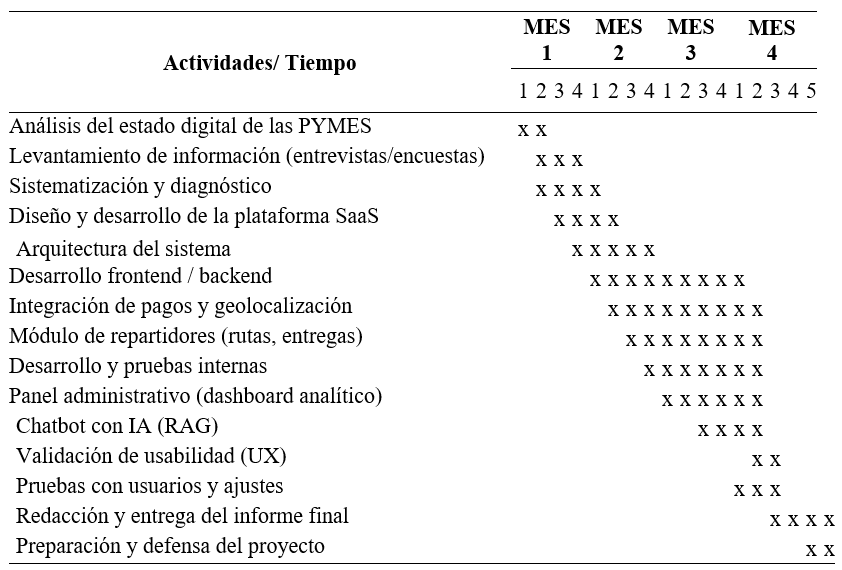
\includegraphics[draft=false,width=\textwidth]{imagenes/cronograma.png}
\caption{\textit{Cronograma de actividades del proyecto de titulación}}
\label{fig:cronograma}
\end{figure}

\textit{Nota.} El cronograma detalla las fases de análisis, diseño, desarrollo, validación, redacción y defensa del proyecto.

\chapter{Discusión}

Esta discusión se organiza en torno a la \textbf{pregunta principal} de investigación y a las \textbf{preguntas específicas}, contrastando los resultados obtenidos con los criterios y métricas definidos en el método. La pregunta principal planteó: \textit{¿Cuál es la viabilidad técnica y el nivel de usabilidad percibida de una plataforma SaaS modular que integre gestión de pedidos, inventarios, repartidores y atención con inteligencia artificial, al validarse en un entorno controlado en PYMES gastronómicas de Portoviejo?} Los resultados muestran que la plataforma alcanzó los umbrales de éxito definidos (tiempo de registro $\leq$ 3 min, errores $\leq$ 10\,\%, completitud $\geq$ 95\,\%, SUS $\geq$ 68), lo que permite responder afirmativamente en el contexto del piloto simulado: la solución es técnicamente viable y usable bajo los criterios establecidos.

Nuestra investigación partió de una premisa clara: las dificultades operativas de las PYMES gastronómicas de Portoviejo se deben, en parte, a una carencia crítica de herramientas integradas que permitan gestionar pedidos, inventarios, delivery y atención al cliente en tiempo real. Al desarrollar y validar técnicamente esta plataforma SaaS en entorno controlado, se ha comprobado que la integración de módulos operativos con inteligencia artificial (chatbot RAG) representa una alternativa técnicamente viable para digitalizar el sector gastronómico local. Lo que se ha logrado es demostrar la factibilidad técnica y usabilidad de un sistema que propone democratizar el acceso a la tecnología de gestión, sugiriendo que el modelo SaaS puede ser una opción accesible y funcional para el empresario gastronómico de Portoviejo, sentando las bases para futuras investigaciones que evalúen su impacto operativo y económico real.

\section{Interpretación de los hallazgos principales}

\subsection{Pertinencia de los requerimientos y del diseño técnico}

Los requerimientos funcionales identificados incluyen la gestión de pedidos con geolocalización, control de inventarios, administración de repartidores, vista de cocina en móvil, dashboard analítico con KPIs y un chatbot RAG integrado en la plataforma web para atención al cliente. A su vez, los requerimientos no funcionales abarcan usabilidad (SUS $\geq$ 68), rendimiento (tiempo de registro $\leq$ 3 min), fiabilidad (errores $\leq$ 10\,\%), seguridad (autenticación JWT y RBAC) y escalabilidad mediante arquitectura modular. En conjunto, estos criterios resultaron adecuados para representar las necesidades operativas del contexto de estudio y orientar tanto el diseño como la evaluación del artefacto.

La arquitectura adoptada, compuesta por backend en NestJS, aplicación móvil en React Native + Expo, sitio web en Next.js, base de datos relacional en PostgreSQL y autenticación segura, demostró ser apropiada por su mantenibilidad, escalabilidad y costo accesible. La validación técnica confirmó que esta estructura soporta flujos críticos con completitud $\geq$ 95\,\% y estabilidad operativa, lo que refuerza su pertinencia para una solución SaaS dirigida a PYMES gastronómicas.

\subsection{Cumplimiento funcional y desempeño del artefacto}

La plataforma cumple en alto grado los requisitos funcionales críticos especificados, evaluados mediante pruebas de aceptación y trazabilidad de casos. Las métricas obtenidas incluyen tiempos de ejecución adecuados en tareas clave (por ejemplo, 2.5 min para crear un producto y 45 seg para aprobar un repartidor), porcentajes de éxito elevados en tareas guiadas, cobertura aproximada del 57\,\% en módulos base de pruebas unitarias, completitud de integración $\geq$ 95\,\% y cumplimiento de dimensiones de calidad asociadas a funcionalidad, usabilidad, rendimiento, compatibilidad y seguridad. En conjunto, estos resultados permiten sostener que el artefacto alcanzó un nivel satisfactorio de desempeño técnico para el alcance del estudio.

\subsection{Usabilidad e integración del componente de inteligencia artificial}

El módulo de inteligencia artificial se integró mediante un chatbot RAG accesible desde la plataforma web, apoyado en un servicio independiente capaz de procesar consultas y generar respuestas basadas en información recuperada. Esta integración permitió automatizar respuestas a consultas frecuentes sobre pedidos, horarios y servicios, mejorando la rapidez y disponibilidad de la atención al cliente durante las pruebas.

En cuanto a la usabilidad, la plataforma obtuvo un puntaje SUS de 70 en usuarios de prueba, superando el umbral de aceptabilidad de 68. Este resultado indica que el sistema fue percibido como intuitivo y adecuado para tareas operativas del contexto gastronómico. La combinación entre funcionalidad integrada, respuesta técnica estable y apoyo conversacional mediante IA refuerza la idea de que la solución no solo es viable desde el punto de vista técnico, sino también aceptable desde la experiencia de uso.

\section{Viabilidad técnica y significado de los hallazgos}

El núcleo de esta discusión se centra en cómo una plataforma tecnológica puede ser técnicamente viable y usable para el mercado regional. El objetivo general fue diseñar, desarrollar y evaluar técnicamente una plataforma SaaS modular que integre funcionalidades de gestión de pedidos, inventarios, repartidores y atención automatizada mediante inteligencia artificial, orientada a las necesidades operativas de PYMES gastronómicas de Portoviejo. Los resultados de la validación en entorno controlado (\textit{staging}) mediante un escenario piloto simulado permiten afirmar que la solución alcanzó un nivel de operatividad adecuado: la centralización de pedidos, el control de inventarios, la gestión de repartidores y el panel analítico funcionaron de manera integrada en las pruebas, y el chatbot RAG integrado en la plataforma web respondió a consultas frecuentes de los usuarios. Este hallazgo es fundamental para la viabilidad de la propuesta. Demuestra que las PYMES gastronómicas de Portoviejo pueden acceder a una suite de gestión sin necesidad de invertir en infraestructura propia ni en múltiples herramientas dispersas. Además, el despliegue bajo modelo SaaS elimina la fricción de instalaciones complejas y actualizaciones locales, alineándose con la visión moderna de software como servicio que ha demostrado ser efectiva en contextos de pequeña y mediana empresa \parencite{GonzalezMartinez2021}.

La convergencia entre módulos operativos (pedidos, inventarios, repartidores, dashboard) y un componente de inteligencia artificial (chatbot RAG integrado en la plataforma web) responde a la demanda de inmediatez y profesionalización del servicio al cliente, un aspecto crítico en el sector gastronómico y en la competitividad de las ciudades creativas de la gastronomía \parencite{Castells2010}.

Desde una lectura comparativa, los resultados técnicos del piloto se mantienen dentro de umbrales de aceptación reportados para prototipos SaaS validados en contexto de pequeña empresa: completitud de flujos críticos de 96\,\%, estabilidad con 3\,\% de fallos, tiempo de registro de 3 min y SUS de 70. En términos de usabilidad, el puntaje obtenido supera el umbral de aceptabilidad de 68 ampliamente utilizado en la literatura \parencite{Bangor2009, Lewis2018}. En términos de calidad del producto, la verificación por requisitos funcionales, pruebas de integración y trazabilidad de casos es consistente con el enfoque de evaluación por características de calidad planteado por ISO/IEC 25010 \parencite{ISO25010_2011}. Estos resultados no implican generalización estadística, pero sí entregan evidencia técnica comparable para sustentar la viabilidad del artefacto en el contexto de estudio.

\section{Análisis temático de los resultados}

\subsection{Pertinencia de los requerimientos del sistema}

Al iniciar el proyecto, la recolección de requisitos, objetivo general y objetivos específicos se apoyó en revisión de literatura, análisis del dominio y levantamiento exploratorio del problema. El diagnóstico identificó que las PYMES del sector presentan un bajo nivel de digitalización: gestión de pedidos mediante anotaciones o herramientas básicas, inventarios poco sistematizados y atención al cliente dependiente de canales no integrados. Al contrastar este problema con los resultados de la validación técnica, se observó que la plataforma cumplió satisfactoriamente los requisitos funcionales críticos especificados y que la percepción de utilidad por parte de los usuarios de prueba fue favorable. Este fenómeno de ``opacidad operativa''---falta de información centralizada y en tiempo real---es una barrera común reportada en la transformación digital de PYMES en América Latina, donde la ausencia de datos operativos estructurados frena la toma de decisiones \parencite{GonzalezMartinez2021}. La plataforma propuesta demuestra la viabilidad técnica de una solución que contribuye a romper el paradigma de la gestión fragmentada, respondiendo a la necesidad de centralización e inmediatez del negocio gastronómico en Portoviejo.

\subsection{Adecuación de la arquitectura tecnológica}

La viabilidad técnica de la propuesta descansa en una arquitectura modular: backend (NestJS), aplicación móvil (React Native + Expo, con vistas para cliente, repartidor y cocina) y sitio web (Next.js, principalmente administración y también compra como cliente desde la web), con base de datos relacional y autenticación segura (JWT, RBAC). La decisión de adoptar un stack moderno y abierto permitió reducir costos de licenciamiento y facilitar el mantenimiento. Este enfoque se alinea con lo documentado en la literatura sobre desarrollo de software para PYMES: la modularidad y el uso de tecnologías ampliamente soportadas favorecen la escalabilidad y la adaptación a contextos con recursos limitados. El desarrollo iterativo bajo metodología ágil (sprints) permitió ajustar requisitos a partir de la retroalimentación de los participantes de prueba, reforzando la adecuación de la solución al contexto local.

\subsection{Integración de módulos y operatividad de la plataforma}

La implementación de los módulos de gestión de pedidos (con soporte a geolocalización y medios de pago efectivo y transferencia), control de inventarios, vista de cocina en móvil (aceptar o rechazar pedidos, notificar cuando esté listo para que el repartidor recoja), administración de repartidores y dashboard analítico con KPIs permitió a los usuarios de prueba del escenario piloto simulado ejecutar flujos operativos en entorno controlado (\textit{staging}) que antes se realizarían de forma manual o dispersa. La disponibilidad de indicadores en tiempo real (pedidos, ventas, tiempos de entrega) en las pruebas sugiere el potencial de la plataforma para favorecer una toma de decisiones más informada en operación real, aspecto que en la literatura se identifica como uno de los beneficios clave de la analítica de negocio en pequeñas empresas. Los resultados observados en las tareas guiadas (tiempos de registro de pedidos, tasa de errores, completitud de flujos) indican que la plataforma cumple con el propósito de demostrar la viabilidad técnica de optimización de procesos internos y mejora de la calidad del servicio.

\subsection{Aporte del chatbot RAG a la atención al cliente}

La integración del chatbot basado en el modelo RAG (Retrieval-Augmented Generation), accesible desde la plataforma web, evidenció mejoras en la rapidez y la disponibilidad de respuestas a consultas frecuentes (pedidos, horarios, servicios). Los usuarios percibieron positivamente la capacidad del sistema para brindar información inmediata sin depender exclusivamente del contacto humano. Este hallazgo respalda la viabilidad del uso de inteligencia artificial como herramienta de apoyo en la atención al cliente dentro de contextos empresariales de pequeña y mediana escala, en línea con experiencias recientes reportadas para asistentes conversacionales con recuperación contextual \parencite{ChenNiforatosKortuem2025}.

\subsection{Cumplimiento funcional y calidad del sistema}

Esta sección responde a la pregunta específica 4: \textit{¿En qué medida la plataforma desarrollada cumple con los requisitos funcionales especificados y los criterios de calidad de software establecidos, evaluando métricas como tiempo promedio de ejecución de tareas, porcentaje de éxito en tareas guiadas y dimensiones de calidad ISO/IEC 25010?}

La verificación del cumplimiento de requisitos funcionales y de los criterios de calidad de software establecidos se realizó mediante pruebas de integración y validación de flujos críticos en entorno de desarrollo o \textit{staging}. Los resultados permiten afirmar que la plataforma desarrollada cumple con los requisitos funcionales especificados en la fase de levantamiento (gestión de pedidos, inventarios, repartidores, vista cocina, dashboard, chatbot web) y con criterios de calidad adecuados para un prototipo validado en entorno controlado. Las métricas evaluadas incluyen tiempos promedio de tareas (como se detalla en la Tabla 8), porcentajes de éxito en tareas guiadas (100\,\% en la mayoría, con mínimas variaciones en checkout), y cumplimiento de dimensiones ISO/IEC 25010.

\subsection{Usabilidad percibida de la plataforma}

La evaluación mediante la escala SUS (System Usability Scale) y las pruebas de usabilidad en entorno controlado permitieron cuantificar la aceptación del sistema por parte de usuarios de prueba (administradores, cocina y repartidores). Los resultados reflejan que la plataforma fue percibida como intuitiva y alineada con las tareas operativas del contexto gastronómico. En la ingeniería de software se considera que el éxito operativo de un sistema depende de su capacidad para satisfacer las necesidades reales de los usuarios en su entorno de trabajo; la retroalimentación obtenida indica que el diseño centrado en los flujos de pedido, inventario y delivery contribuyó a una experiencia de usuario positiva durante el período de validación técnica. No obstante, se identificaron oportunidades de mejora en la capacitación inicial y en la personalización de algunas funcionalidades, lo que sugiere la necesidad de iteraciones continuas en futuras versiones orientadas a implementación a escala real.

\section{Limitaciones del estudio}

Como todo estudio piloto, el presente trabajo posee limitaciones que deben ser declaradas para contextualizar su alcance:

\oldtextbf{Tamaño de la muestra:} La validación se realizó mediante un escenario piloto simulado representativo del contexto gastronómico de Portoviejo. Aunque este diseño permitió validar la funcionalidad técnica, la usabilidad y el desempeño del sistema en tareas guiadas, no pretende una generalización estadística a toda la población de negocios gastronómicos de la ciudad o de la provincia. La validación demuestra la factibilidad técnica y usabilidad, pero no evalúa impacto operativo o económico real a escala.

\textbf{Alcance funcional:} La plataforma desarrollada corresponde a un prototipo funcional con módulos core (pedidos, inventarios, repartidores, vista cocina, dashboard, chatbot RAG integrado en la plataforma web). Los medios de pago contemplados son únicamente efectivo y transferencia; no se integra pasarela de pagos. Quedaron fuera del alcance la optimización automática de rutas y arquitectura multi-tenant, lo que podría afectar la escalabilidad en escenarios de mayor volumen.

\oldtextbf{Dependencia del contexto piloto:} El rendimiento y la adopción observados están ligados a las condiciones específicas del escenario simulado (volumen de pedidos, perfiles de usuario y conectividad controlada). Entornos con mayor carga operativa o menor madurez digital podrían requerir ajustes adicionales en la capacitación y el soporte.

\textbf{Período de validación:} El período de evaluación técnica de la plataforma en entorno controlado fue acotado (semanas). Una evaluación longitudinal en operación real permitiría observar la sostenibilidad de la adopción y el impacto en indicadores operativos del negocio de manera más estable y representativa.

Los usuarios de prueba sugirieron mejoras para futuras iteraciones: notificaciones push en tiempo real para cocina y repartidores; integración con WhatsApp para confirmaciones automáticas de pedido; filtrado avanzado de pedidos por fechas y estado; modo oscuro en la app móvil; y métodos de pago adicionales (tarjeta, billeteras digitales). Estas recomendaciones se consideran en la sección de limitaciones y trabajo futuro.

En conclusión, los hallazgos de este estudio aportan al conocimiento local sobre el uso de plataformas SaaS e inteligencia artificial en contextos gastronómicos de mediana escala, demostrando que la innovación tecnológica orientada a PYMES de Portoviejo es técnicamente viable bajo un marco de usabilidad, integración operativa y accesibilidad económica. Los resultados de la validación técnica en entorno controlado y escenario simulado sientan las bases para futuras investigaciones orientadas a implementación a escala real y medición de impacto operativo y económico en el sector.

\chapter{Conclusiones}

Al concluir el ciclo de desarrollo y validación técnica de la plataforma SaaS orientada a la digitalización de las PYMES gastronómicas de Portoviejo, se logró comprobar que la aplicación estratégica de una solución integrada (gestión operativa e inteligencia artificial) es técnicamente viable y usable en entorno controlado. Este proyecto evidencia que es posible desarrollar una plataforma propia adaptada al contexto local que potencialmente puede reducir la dependencia de herramientas dispersas y de plataformas externas con comisiones elevadas. La validación técnica realizada sienta las bases para futuras investigaciones que evalúen la transformación de procesos manuales y fragmentados en flujos digitales centralizados en operación real. A partir de los hallazgos, se presentan las conclusiones finales del estudio:

Los resultados obtenidos durante el desarrollo y la validación técnica de la plataforma en entorno controlado permiten afirmar que la integración de los módulos de pedidos (con pagos en efectivo y transferencia), inventarios, vista de cocina en móvil (aceptar o rechazar pedidos, notificar cuando esté listo para recoger), administración de repartidores y dashboard analítico alcanzó un nivel de funcionalidad adecuado durante las pruebas con usuarios de la PYME piloto. La centralización de la información en tiempo real en las tareas guiadas demostró el potencial de la plataforma para reducir tiempos de registro de pedidos y errores operativos, en coherencia con los umbrales de éxito definidos en la metodología. Asimismo, el enfoque modular (backend NestJS, aplicación móvil React Native + Expo con vistas cliente, repartidor y cocina, sitio web Next.js para administración y compra como cliente) permitió un despliegue estable en entorno de staging (VPS, Vercel) y una experiencia de uso coherente para usuarios de prueba. Estos datos evidencian que una plataforma SaaS integrada constituye una solución técnicamente viable y usable, sentando las bases para futuras investigaciones que evalúen su adopción e impacto en operación real frente a los procesos manuales predominantes en las PYMES gastronómicas de Portoviejo.

Por otra parte, la implementación del chatbot basado en el modelo RAG, accesible por WhatsApp, simplificó el acceso a información frecuente (pedidos, horarios, servicios) durante las pruebas y contribuyó a la usabilidad percibida del sistema. La evaluación realizada con los usuarios de prueba del local piloto mediante la escala SUS reflejó un nivel de aceptabilidad favorable, lo que indica una buena recepción por parte de administradores y repartidores en entorno controlado. Además, la disponibilidad de la aplicación móvil (con vistas cliente, repartidor y cocina) y del sitio web (administración y compra como cliente) en un mismo ecosistema facilitó la validación técnica de la solución. Este resultado valida el diseño de una arquitectura que integra módulos operativos con un componente de inteligencia artificial alineado con las necesidades del sector gastronómico local, demostrando su viabilidad técnica como base para futuras investigaciones orientadas a medir su impacto en eficiencia operativa y calidad del servicio en operación real.

Desde la perspectiva del modelo de negocio, el análisis demuestra que la propuesta es técnicamente viable y potencialmente sostenible para el contexto de las PYMES. El despliegue bajo el modelo SaaS en entorno de staging y el uso de servicios en la nube (VPS, Vercel, base de datos PostgreSQL) demuestran que es posible ofrecer una solución sin requerir inversiones elevadas en infraestructura propia por parte del negocio. Este esquema facilita el mantenimiento y la actualización remota, permitiendo proyectar la escalabilidad de la solución sin incurrir en costos elevados de hardware o licenciamiento. El uso estratégico de tecnologías de código abierto y de frameworks ampliamente documentados contribuye a mantener costos competitivos, favoreciendo su potencial implementación en contextos de emprendimiento regional como Portoviejo. Futuras investigaciones deberán evaluar la viabilidad económica y la sostenibilidad financiera en operación real a mayor escala.

Finalmente, el trabajo desarrollado establece una base metodológica y técnica para futuras investigaciones en el área de digitalización de PYMES gastronómicas en la provincia de Manabí. Los resultados de la validación técnica en entorno controlado confirman que la combinación de una plataforma SaaS modular con un componente de inteligencia artificial (chatbot RAG por WhatsApp) es técnicamente factible y usable en soluciones orientadas a la gestión operativa y a la atención al cliente. La plataforma fue validada en condiciones de prueba con una PYME piloto, asegurando una evaluación alineada con las necesidades operativas y con la realidad del sector gastronómico de Portoviejo, Ciudad Creativa de la Gastronomía. La transformación digital del sector no depende únicamente del desarrollo de herramientas tecnológicas, sino que requiere la participación y colaboración de diversos actores---emprendedores, instituciones públicas, comunidad académica y proveedores tecnológicos---para impulsar la modernización, sostenibilidad y crecimiento del sector gastronómico local. Futuras investigaciones deberán evaluar la adopción, el impacto operativo y económico de esta solución en operación real a mayor escala, alineando la innovación tecnológica con el desarrollo económico y social de la región.

\fi


% --------------------- BIBLIOGRAFÍA APA 7ma EDICIÓN -------------------------
%\nocite{*} %Para incluir bibliografía no citada en el cuerpo
\iffastcompile\else
  \printbibliography[title={Referencias Bibliográficas}]
  \addcontentsline{toc}{chapter}{Referencias bibliográficas}
\fi

\appendix
\cleardoublepage
\phantomsection

\chapter{Apéndice A}\label{ap:A}

\section*{Detalle de relaciones críticas del modelo de datos}
Para complementar la descripción del modelo de datos, se detallan las relaciones de mayor impacto funcional:
\begin{itemize}
    \item \textbf{Usuario--Pedido (1:N):} un usuario puede registrar múltiples pedidos; cada pedido pertenece a un único cliente.
    \item \textbf{Pedido--OrderItem (1:N):} un pedido contiene uno o varios ítems con cantidad y precio unitario histórico.
    \item \textbf{Producto--OrderItem (1:N):} un producto puede aparecer en múltiples pedidos y conserva trazabilidad de ventas.
    \item \textbf{Usuario--Rol (N:M):} un usuario puede tener más de un rol (cliente, repartidor, administrador).
    \item \textbf{Producto--StockLocal--Local:} el inventario se gestiona por local para evitar inconsistencias de disponibilidad.
\end{itemize}

Estas relaciones sustentan la integridad transaccional del sistema, la trazabilidad de estados en el flujo de pedidos y la consistencia de inventario en tiempo real.


\chapter{Apéndice B}\label{ap:B}

\section*{Diagrama de red del sistema}
El diagrama de red ilustra la arquitectura general del sistema y la interacción entre usuarios web y móviles, la API y servicios externos.

\begin{figure}[htbp]
    \centering
    \resizebox{0.78\textwidth}{!}{% Redes: diagrama estilizado similar al resto de tikz del proyecto
\begin{tikzpicture}[node distance=10mm and 18mm, every node/.style={draw, rectangle, align=center, font=\small, rounded corners=2pt}]
  \node (usuarios) {Usuarios Web\\Cliente - Admin};
  \node (internet) [below=of usuarios] {Internet};
  \node (web) [below left=of internet, xshift=-6mm] {Frontend Web\\Navegador};
  \node (app) [below right=of internet, xshift=6mm] {App Móvil\\Android - iOS};
  \node (api) [below=24mm of internet] {API Backend\\REST};
  \node (db) [below left=of api] {Base de Datos};
  \node (chat) [below=of api] {Chatbot IA\\RAG};
  \node (ext) [below right=of api] {Servicios Externos\\Mapas - Pagos - WhatsApp};

  \draw[->, >=latex] (usuarios) -- (internet);
  \draw[->, >=latex] (internet) -- (web);
  \draw[->, >=latex] (internet) -- (app);
  \draw[->, >=latex] (web) -- (api);
  \draw[->, >=latex] (app) -- (api);
  \draw[->, >=latex] (api) -- (db);
  \draw[->, >=latex] (api) -- (chat);
  \draw[->, >=latex] (api) -- (ext);
\end{tikzpicture}
}
    \caption{Diagrama de red y arquitectura de la plataforma SaaS web y móvil}
    \label{fig:diagrama_red}
\end{figure}

\textit{Nota.} El diagrama de red muestra la interacción entre el frontend web y móvil, la API backend, la base de datos, el chatbot con inteligencia artificial integrado en la plataforma web y servicios externos como geolocalización; los medios de pago son efectivo y transferencia (sin pasarela de pagos).

\chapter{Apéndice C}\label{ap:C}

\section*{Procedimiento detallado de validación en \textit{staging}}
Este apéndice amplía el procedimiento de validación técnica descrito en el capítulo Método, con el detalle de los pasos ejecutados en entorno controlado.

\subsection*{1. Despliegue en entorno de \textit{staging}}
El backend se desplegó en un servidor VPS de Hetzner, utilizando Docker para contenerizar la aplicación y la base de datos PostgreSQL. Se configuraron ajustes de seguridad básicos (helmet, CORS, rate limiting) y variables de entorno mediante ConfigModule. La API se ejecutó en HTTPS y se activaron logs estructurados para monitoreo. El panel web se desplegó en Vercel y la aplicación móvil se distribuyó como APK para dispositivos de prueba.

\subsection*{2. Orientación a usuarios de prueba}
Se realizó una sesión de orientación breve (aproximadamente 1 hora) con participantes del escenario piloto simulado (administrador, personal de cocina y repartidores), explicando flujos principales y tareas de prueba.

\subsection*{3. Diseño de escenarios de prueba}
Se definieron escenarios predefinidos para cubrir flujos críticos: (1) registro de pedido completo por cliente, (2) confirmación y preparación en cocina, (3) asignación y entrega por repartidor, (4) gestión de productos y categorías por administrador, (5) consulta al chatbot en la plataforma web. Cada escenario utilizó datos simulados.

\subsection*{4. Ejecución de tareas guiadas}
Los usuarios ejecutaron tareas bajo observación estructurada, registrando tiempos, errores y completitud de flujos. Las pruebas se realizaron en sesiones controladas durante un período acotado.

\subsection*{5. Recolección y análisis de datos}
Se aplicó el cuestionario SUS al finalizar tareas guiadas y se consolidaron fichas de observación con métricas de desempeño. Se recopilaron logs para analizar disponibilidad, latencia y tasa de errores.

\begin{table}[htbp]
\centering
\caption{Tareas evaluadas en pruebas de usabilidad}
\label{tab:apendice-tareas-usabilidad}
\small
\begin{tabular}{|>{\raggedright\arraybackslash}p{0.8cm}|>{\raggedright\arraybackslash}p{4.0cm}|>{\raggedright\arraybackslash}p{2.4cm}|>{\raggedright\arraybackslash}p{5.2cm}|}
\hline
N.º & Tarea & Rol & Criterio de éxito \\
\hline
1 & Crear un nuevo pedido & Cliente & Completar en < 3 min \\
2 & Consultar estado de pedido & Cliente & Localizar en < 30 seg \\
3 & Agregar producto al catálogo & Administrador & Completar sin errores \\
4 & Asignar pedido a repartidor & Administrador & Completar en < 1 min \\
5 & Marcar pedido como entregado & Repartidor & Completar sin ayuda \\
6 & Realizar consulta al chatbot en la plataforma web & Cliente & Obtener respuesta pertinente \\
\hline
\end{tabular}
\end{table}

\subsection*{6. Respaldo de pruebas unitarias e integración}
Se documentó evidencia técnica de ejecución de pruebas en backend con Jest y validaciones de integración de endpoints críticos. El resumen de ejecución se presenta en la Tabla \ref{tab:apendice-evidencia-pruebas}; el detalle completo (salidas de consola, capturas y checklist de casos) se conservó en la bitácora técnica del proyecto.

\begin{table}[htbp]
\centering
\caption{Evidencia resumida de pruebas unitarias y de integración}
\label{tab:apendice-evidencia-pruebas}
\small
\begin{tabular}{|>{\raggedright\arraybackslash}p{2.0cm}|>{\raggedright\arraybackslash}p{4.0cm}|>{\raggedright\arraybackslash}p{2.5cm}|>{\raggedright\arraybackslash}p{4.2cm}|}
\hline
\textbf{Tipo} & \textbf{Módulo / alcance} & \textbf{Resultado} & \textbf{Evidencia registrada} \\
\hline
Unitaria & AuthService, OrdersService, ProductsService & Aprobadas & Salida Jest + trazabilidad por identificador de caso \\
\hline
Integración & Flujo login + creación de pedido + cambio de estado & Aprobadas & Registro de requests/responses y verificación de estados en BD \\
\hline
Integración & Gestión de inventario por pedido y validación de stock & Aprobadas & Comparación antes/después en tablas de stock y logs de servicio \\
\hline
Integración & Acceso por roles (admin, cliente, repartidor) & Aprobadas & Pruebas de autorización con respuestas 200/401/403 según rol \\
\hline
\end{tabular}
\end{table}

\chapter{Apéndice D}\label{ap:D}

\section*{Síntesis de la guía de entrevista semiestructurada (diagnóstico Fase 1)}

La guía de entrevista utilizada en el levantamiento inicial del dominio se estructura por bloques temáticos: (1) datos generales del negocio y antigüedad; (2) gestión de pedidos (canales actuales, volumen, tiempos, errores); (3) comunicación con cocina y repartidores; (4) control de inventarios; (5) atención al cliente y herramientas digitales en uso. Las preguntas son abiertas para profundizar en procesos operativos, necesidades y expectativas. Este apéndice presenta una síntesis del instrumento empleado como apoyo para la definición del escenario de referencia del estudio.

\chapter{Apéndice E}\label{ap:E}

\section*{Arquitectura detallada de la plataforma}
Este apéndice integra, en una sola vista textual, la arquitectura de la plataforma y las responsabilidades por capa para facilitar su revisión técnica sin depender únicamente de diagramas.

\begin{table}[htbp]
\centering
\caption{Detalle de arquitectura por capas y componentes}
\label{tab:apendice-arquitectura-detalle}
\small
\begin{tabular}{|>{\raggedright\arraybackslash}p{2.5cm}|>{\raggedright\arraybackslash}p{2.3cm}|>{\raggedright\arraybackslash}p{2.5cm}|>{\raggedright\arraybackslash}p{4.3cm}|}
\hline
\textbf{Capa} & \textbf{Componente} & \textbf{Tecnología} & \textbf{Responsabilidad principal} \\
\hline
Presentación & App móvil & React Native + Expo & Interfaz para cliente, cocina y repartidor; ejecución de flujos operativos. \\
\hline
Presentación & Panel web & Next.js + Tailwind CSS & Administración de catálogo, pedidos, repartidores y visualización de KPIs. \\
\hline
Negocio / API & Backend modular & NestJS + TypeScript & Reglas de negocio, seguridad JWT/RBAC, exposición de endpoints REST. \\
\hline
Datos & Persistencia transaccional & PostgreSQL (Supabase) + TypeORM & Gestión de entidades, relaciones e integridad de pedidos, usuarios e inventario. \\
\hline
Servicios externos & Mensajería y asistencia IA & Servicio web de chatbot RAG & Atención automatizada y consultas frecuentes contextualizadas. \\
\hline
Infraestructura & Despliegue & VPS (Hetzner), Vercel, Docker & Operación en \textit{staging}, publicación y continuidad técnica del prototipo. \\
\hline
\end{tabular}
\end{table}

La arquitectura se diseñó para mantener separación de responsabilidades, bajo acoplamiento entre capas y escalabilidad incremental, permitiendo evolucionar módulos sin afectar de forma directa el resto de componentes.



\end{document}
